\documentclass[10pt]{report}
\usepackage[utf8]{inputenc}
\usepackage[italian]{babel}
\usepackage{multicol}
\usepackage{amsfonts}
\usepackage{amsmath}
\usepackage[bookmarks]{hyperref}
\usepackage[a4paper, total={18cm, 25cm}]{geometry}
\usepackage{graphicx}
\usepackage{xcolor}
\usepackage{textcomp}
\graphicspath{ {./img/} }
\usepackage{listings}
\usepackage{makecell}
\usepackage{mathrsfs}
\usepackage{cancel}

\definecolor{backcolour}{RGB}{255,255,255}
\definecolor{codegreen}{RGB}{27,168,11}
\definecolor{codeblue}{RGB}{35,35,205}
\definecolor{codegray}{RGB}{128,128,128}
\definecolor{codepurple}{RGB}{205,35,56}
\lstdefinestyle{myPython}{
	backgroundcolor=\color{backcolour},   
	commentstyle=\color{codegreen},
	keywordstyle=\color{codeblue},
	numberstyle=\tiny\color{codegray},
	stringstyle=\color{codepurple},
	basicstyle=\small\ttfamily,
	breakatwhitespace=false,         
	breaklines=true,                 
	captionpos=b,                    
	keepspaces=true,                 
	numbers=left,                    
	numbersep=2pt,                  
	showspaces=false,                
	showstringspaces=false,
	showtabs=false,                  
	tabsize=2,
	language=python
}

\usepackage{fancyhdr}
\pagestyle{fancy}
\renewcommand{\headrulewidth}{0pt}
\fancyhead{}
\fancyfoot[L]{Telegram: \texttt{@fexed}}
\fancyfoot[R]{Github: \texttt{fexed}}
\begin{document}
\title{Computational Mathematics for Learning and Data Analysis}
\author{Federico Matteoni}
\date{A.A. 2023/24}
\renewcommand*\contentsname{Index}

\maketitle
\tableofcontents
\pagebreak
\section{Introduction}
\paragraph{Exam} Typical project, usually in groups of 2 students, followed by an oral exam. No fixed dates, and the project should be submitted incrementally. Once the project is complete, an oral date is decided.
\paragraph{Course} The goal is to make sense of the huge amounts of data: to \textbf{take something big and unwieldy and produce something small that can be used}, a \textbf{mathematical model}.\\
The mathematical model should be \textbf{accurate}, \textbf{computationally inexpensive} and \textbf{general}, but generally is \textbf{not possible to have all three}. General models are convenient (\textit{work once, apply many}), they are parametric so we need to learn the right values of the parameters for the particular instance at hand. \textbf{Fitting} is the process of \textbf{finding the model that better represents the phenomenon given a family of possible models}, which usually are infinitely many. Is an \textbf{optimization problem} and usually this is the computational bottleneck.\\
Machine Learning is better than fitting because \textbf{fitting reduces the training error}, the empirical risk, but \textbf{Machine Learning reduces the test error}, so the generalization error.\\
Solve general problem $$\min_{x\in S}f(x)$$ or a particular version $$\min_{x\in \mathbb{R}^n}\|Ax - b\|_2$$ which is easier and can be solved exactly.
\begin{center}
	
\includegraphics[scale=0.75]{xkcd_1838.png}\\
	XKCD 1838
\end{center}
\paragraph{Languages} Matlab, Python, C and \textit{Fortran}
\chapter{Numerical Analysis}
\section{Quick recap of linear algebra}
\begin{list}{}{}
	\item \textbf{Matrix - Vector multiplication}, with $A\in \mathbb{R}^{4\times 3}, c\in \mathbb{R}^3, b\in \mathbb{R}^4$ \textbf{row-by-column}
	$$\left[\begin{array}{c c c}
		A_{11} & A_{12} & A_{13}\\
		\vdots & \vdots & \vdots\\
		A_{41} & A_{42} & A_{43}
	\end{array}\right]\cdot \left[\begin{array}{c}
		c_1\\c_2\\c_3
	\end{array}\right] = \left[\begin{array}{c}
		b_1\\b_2\\b_3\\b_4
	\end{array}\right]\:\:\:\:\:\:\begin{array}{l}
		b_i = \sum_{j} A_{ij}c_j\\
		\text{e.g. }A_{11}c_1 + A_{12}c_2 + A_{13}c_3 = b_1
	\end{array}$$
	or linear combination of the columns
	$$\left[\begin{array}{c}
	A_{11}\\A_{21}\\A_{31}\\A_{41}
	\end{array}\right]c_1 + \left[\begin{array}{c}
	A_{12}\\A_{22}\\A_{32}\\A_{42}
	\end{array}\right]c_2 + \left[\begin{array}{c}
	A_{13}\\A_{23}\\A_{33}\\A_{43}
	\end{array}\right]c_3 + \left[\begin{array}{c}
	A_{14}\\A_{24}\\A_{34}\\A_{44}
	\end{array}\right]c_4 = \left[\begin{array}{c}
	b_1\\b_2\\b_3\\b_4
	\end{array}\right]$$
	with $c_1, c_2, c_3$ and $c_4$ called coordinates.
	\item \textbf{Matrix - Matrix multiplication}, with a useful mnemonic: if the inner dimensions agree, the product is well-defined and removes them. An example:
	$$A\in\mathbb{R}^{4\times3}, B\in\mathbb{R}^{3\times2} \Rightarrow AB\in\mathbb{R}^{4\times2}$$
	So the ordering is very important as well as the use of the parenthesis. Keep in mind this, as $AB=AC \not\Rightarrow B=C$ and $AB\neq BA$ in general.
	\item \textbf{Basis}: tuple of vectors $v_1, v_2, \ldots, v_n$ such that you can write all vectors $b$ in a certain space as a linear combination of $v_i$: $v_1\alpha_1 + v_2\alpha_2 + \ldots + v_n\alpha_n$ with \textbf{unique} $a_1,\ldots,a_n$. The canonical basis is 
	$$c_1 = \left[\begin{array}{c}
	1\\0\\0\\0
	\end{array}\right]\:\:\:c_2 = \left[\begin{array}{c}
	0\\1\\0\\0
	\end{array}\right]\:\:\:c_3 = \left[\begin{array}{c}
	0\\0\\1\\0
	\end{array}\right]\:\:\:c_4 = \left[\begin{array}{c}
	0\\0\\0\\1
	\end{array}\right]$$
	and, for example $$\left[\begin{array}{c}
	3\\5\\7\\9
	\end{array}\right] = \left[\begin{array}{c}
	1\\0\\0\\0
	\end{array}\right]\cdot 3 + \left[\begin{array}{c}
	0\\1\\0\\0
	\end{array}\right]\cdot 5 + \left[\begin{array}{c}
	0\\0\\1\\0
	\end{array}\right]\cdot 7 + \left[\begin{array}{c}
	0\\0\\0\\1
	\end{array}\right]\cdot 9$$
	\item \textbf{Image} $\text{Im} A$ = set of vectors $b$ that we can reach with $A$ as operator, meaning all $y\:|\:\exists\:x\:\:Ax=y$
	\item \textbf{Kernel} $\text{Ker} A$ = set of vectors $x\:|\: Ax = 0$ ($x = 0$ is certainly one, there may be others)
	\item \textbf{Rank} $\text{rk}A$ has a precise meaning in linear algebra: the rank of a matrix is the minimum $r$ so that we can find vectors $v_1,\ldots,v_r$ such that all columns (or rows) of $A$ are linear combinations of these vectors.
	\item \textbf{Invertible} $A$ is invertible if $Ax=y$ has exactly one solution.\\
	This means that $A$ must be square and the columns of $A$ are a basis of $\mathbb{R}^m$.\\
	We can derive $x=A^{-1}b$ where $A^{-1}$ is another square matrix such that $A\cdot A^{-1} = A^{-1}\cdot A = I$, the identity matrix (1 on the diagonal, 0 otherwise)
	\item \textbf{Cost}, with $A\in \mathbb{R}^{m\times n}, B\in \mathbb{R}^{n\times p}, C\in \mathbb{R}^{m\times p}$ (vectors $\Leftrightarrow n\times 1$ matrices), then the cost of multiplication is $mp(2n-1)$ floating point ops (\textit{flops}), or $O(mnp)$.\\
	In particular, $A, B$ squared $\Rightarrow AB$ costs $O(m^3)$. With $A, v$ vector $\Rightarrow$ $Av$ costs $O(m^2)$. Faster alternatives are not worth it usually. And remember that $AB \neq BA$ generally, and also that $CA = CB \not\Rightarrow A = B$ with $C$ matrix.\\
	If there's $M\:|\: MC = I$, then $A = (MC)A = (MC)B = B$ (multiplying \textit{on the left} by $M$ on both sides)
\end{list}
\paragraph{Why a real valued function?} Strong assumption, given $x'$ and $x''$, I can always tell which one I like best (a consequence of the \textbf{total order} property of $\mathbb{R}$). Often more than one objective function, with contrasting and/or incomparable units (ex: loss function vs regularity in ML).\\
But $\mathbb{R}^k$ with $k > 1$ has no total order, so there's no \textit{best} solution, only non-dominated ones.\\
Even with a single objective function, optimization is hard, impossible if $f$ has no minimum in $X$ (meaning that the problem $P$ is unbounded below). Hardly ever happens in ML, because losses and regularizations are $\geq 0$\\
Also impossible if $f > -\infty$ but $\not\exists\:x$, for example in $f(x) = e^x$. However plenty of $\epsilon$-approximate solutions (\textbf{$\epsilon$-optima}). On computers, $x\in \mathbb{R}$ is in fact $x\in \mathbb{Q}$ with up to 16 digits precision, so approximation errors are unavoidable anyway. Exact algebraic computation is possible but usually slow, and ML is going the opposite way (less precision: floats, half, small integer weights\ldots).\\
Anyway, \textbf{finding the exact $x_*$ is impossible in general}, and more often than not we are happy with a "good enough" solution.
\paragraph{Norms} A norm is a way to measure the length or the distance from $0$ of a vector. A norm has the following properties:
\begin{list}{}{}
	\item $\|v\| \geq 0$, and $\|v\|=0\Leftrightarrow v = 0$
	\item $\|v\alpha\|=\|v\|\cdot|\alpha|$ for $\alpha\in\mathbb{C}$
	\item $\|v+w\| \leq \|v\|+\|w\|$
\end{list}
There are many kinds of norm:
\begin{list}{}{}
	\item $\|v\|_{\infty} = \max_i|v_i|$
	\item $\|v\|_1 = \sum_i|v_i|$
	\item $\|v\|_2 = \sqrt{v_1^2+\ldots+v_m^2} = \sqrt{v^Tv} = \sqrt{\langle x,x\rangle}$
\end{list}
The last one is our preferred one, and often the index $_2$ is omitted. Many matrices preserve norm 2.
\paragraph{Orthogonal} A square matrix $U\in \mathbb{R}^{n\times n}$ is orthogonal if $U^TU = I \Leftrightarrow UU^T = I \Leftrightarrow U^{-1} = U^T$ equivalently.
\subparagraph{Theorem} For an orthogonal matrix $U\in \mathbb{R}^{n\times n}$ and every vector $x$, $\|Ux\| = \|x\|$ (meaning norm $_2$ with the index omitted, like from here onward).\\
More generally, $x^T y = (Ux)^T(Uy)$ for all vectors $x,y\in \mathbb{R}^n$.\\
The columns (or the rows) of a orthogonal matrix are \textbf{orthonormal}: $u_i^Tu_j = \left\{\begin{array}{l l}
1 &\text{if } i = j\\0&\text{otherwise}
\end{array}\right.$\\
If $U,V\in \mathbb{R}^{n\times n}$ are orthogonal $\Rightarrow UV$ is orthogonal
\paragraph{Eigenvalues and eigenvectors} Given a square matrix $A\in \mathbb{R}^{m\times m}$, if $Av = \lambda v$ for $v\in \mathbb{R}^m, \lambda\in \mathbb{R}$ then we call $\lambda$ and \textbf{eigenvalue} and $v$ an \textbf{eigenvector} of $A$.\\
For many matrices we can find $v_1,\ldots,v_m$ eigenvectors that are a basis of $R^m$, i.e. $[v_1|\ldots|v_m] = V$ is invertible.\\
$$A = V\cdot\Lambda\cdot V^{-1}\Leftrightarrow AV = V\Lambda\text{, with }\Lambda = \left[\begin{array}{c c c}
\lambda_1 & & 0\\
& \ddots \\
0& & \lambda_m
\end{array}\right]$$
Given $x\in \mathbb{R}^m$ I can write $x = v_1\alpha_1 + \ldots + v_m\alpha_m$ then it's easy to compute the coordinates $Ax = A(v_1\alpha_1 + \ldots + v_m\alpha_m) = v_1(\lambda_1\alpha_1) + \ldots + v_m(\lambda_m\alpha_m)$. Also $A^kx = v_1(\lambda_1^k\alpha_1) + \ldots + v_m(\lambda_m^k\alpha_m)$\\
Eigenvalue decompositions is not unique for all matrices. If $v$ is an eigenvector, then $v\cdot\alpha$ is still one, and if $v,w$ are eigenvectors of the same eigenvalue then $v+w$ is still an eigenvector of the same eigenvalue, and the same hold for any linear combination $\alpha v+\beta w$. Some matrices have complex eigenvalues/eigenvectors only, and some do not have enough eigenvectors to make a basis.
\paragraph{Symmetry} $A$ is symmetric if $A = A^T$
\paragraph{Spectral Theorem} For a symmetric matrix $A\in \mathbb{R}^{m\times m}$ we can always write $A = U\Lambda U^{-1}$
% END 1-linalg
\paragraph{Quadratic form} Given a symmetric matrix $Q = Q^T \in \mathbb{R}^{m\times m}$ we can consider the function $$x\in \mathbb{R}^m\mapsto f(x) = x^T Qx \in \mathbb{R}$$
\subparagraph{Theorem} For all symmetric matrix $Q \in \mathbb{R}^{m\times m}$, $\lambda_{\min}\|x\|^2 \leq x^TQx\leq \lambda_{\max}\|x\|^2$, where $\lambda_{\min}, \lambda_{\max}$ are the smallest and largest eigenvalue of $Q$.
\paragraph{Positive Semidefinite} $Q = Q^T$ is positive semidefinite ($Q \succeq 0$) if all eigenvalues $\lambda_i \geq 0 \Leftrightarrow \lambda_{\min} \geq 0$ hence $x^T Q x\geq 0$ for all $x\in \mathbb{R}^m$\\
Positive definite ($Q \succ 0$) if all eigenvalues $\lambda_i > 0 \Leftrightarrow \lambda_{\min} > 0$ hence $x^TQx > 0$ for all $x \in \mathbb{R}^m, x\neq 0$
\paragraph{Recall theorem} $\lambda_{\min}(x^T x) \leq x^T Q x \leq \lambda_{\max}(x^T x)$ for all symmetric $Q$ so $\lambda_{\min} \leq \frac{x^T Q x}{x^T x} \leq \lambda_{\max}$\\
Slightly different form $\lambda_{\min} \leq z^T Q z \leq \lambda_{\max}$ for all vectors $z$ with $\|z\| = 1$. Equivalent to the other form with $x = \alpha z$, for $\alpha = \|x\|$ and a vector $z$ with $\|z\| = 1$
$$ \frac{x^T Q x}{x^T x} = \frac{(\not\alpha z)^T Q (\not\alpha z)}{\not\alpha^{\not 2}}$$
\paragraph{Generalization for complex matrices} $\|x\|^2 = |x_1|^2 + \ldots + |x_n|^2$, $x^T \longrightarrow \overline{x^T} = x^*$. For orthogonal matrices $U^*U=I \Rightarrow U$ is unitary. For symmetry $Q^* = Q \Rightarrow Q$ is Hermitian.
% END 2-orthogonality
\section{SVD}
\paragraph{Singular Value Decomposition} Each $A\in \mathbb{R}^{n\times n}$ can be decomposed as $A = U\Sigma V^T$ with $U, V$ orthogonal and $\Sigma$ diagonal with $\sigma_1 \geq \ldots \geq \sigma_n \geq 0$.\\
The first notable difference is it exists for every square matrix. The second difference is $V^T$ which is not the inverse of $U$.\\
Another notation is $[u_1|u_2|\ldots|u_m]\left[\begin{array}{c c c c}
\sigma_1\\ & \sigma_2\\ & & \ddots\\ & & & \sigma_m
\end{array} \right]\left[\begin{array}{c}
v_1^T\\v_2^T\\\vdots\\v_m^T
\end{array} \right] = u_1\sigma_1 v_1^T + \ldots + u_m\sigma_m v_m^T$ sum of $m$ rank-1 matrices\\
\subparagraph{Geometric idea} There is an orthogonal basis $v_1,\ldots, v_m$ so that $A$ maps $\{v_i\}$ into multiples of another orthogonal basis $A v_i = u_i \sigma_i$\\
$\{\sigma_i\}$: singular values of $A$, \textbf{defined uniquely for each $A$}. Singular values are not eigenvalues: they are always positive and usually more "spread apart".\\
\subparagraph{Rectangular SVD} Each $A\in \mathbb{R}^{m\times n}$ can be decomposed as $A = U\Sigma V^T$ where $U\in \mathbb{R}^{m\times m}$, $V \in \mathbb{R}^{n\times n}$ are orthogonal and $\Sigma\in \mathbb{R}^{m\times n}$ is diagonal, so there's a padding $\sigma_{i,j} = 0$ whenever $i\neq j$ again with $\sigma_1 \geq \ldots \geq \sigma_{\min(m, n)} \geq 0$\\
So only the first $n$ vectors of $U$ matches with non-zero values in $\Sigma$, all the last $n-m$ columns combine with zeroes.\\
$= u_i\sigma_1 v_1^T + \ldots + u_n \sigma_n v_n^T$ with $u_{n+1},\ldots, u_m$ not used. So we can "chop off" the unused parts and get the same result.\\
$= u_i\sigma_1 v_1^T + \ldots + u_{\min(m, n)} \sigma_{\min(m, n)} v_{\min(m, n)}^T$
\subparagraph{Cost in Malab} \texttt{svd(A, 'econ')} costs $\max(m,n)\cdot \min(m,n)^2$, still cubic but linear in the largest dimension.\\
The full \texttt{[U, S, V] = svd(A)} cannot be linear because one of the outputs will be a huge orthogonal matrix of $\max(m,n)\times \max(m,n)$, so it will cost more in time and memory.
\subparagraph{Properties} The SVD reveals rank, image and kernel of a matrix.
\begin{list}{}{}
	\item \textbf{Rank}\\
The rank of a matrix $A$ is equal to the number of non-zero $\sigma_i$. $\sigma_1\geq \ldots\geq\sigma_r > \sigma_{r+1} = \ldots = \sigma_{\min(m,n)} = 0$
	\item \textbf{Image}\\
	For each $x\in\mathbb{R}^n, Ax$ is a linear combination of $u_1,\ldots,u_r$
	\item \textbf{Kernel}\\
	Any linear combination $y$ of $v_{r+1},\ldots,v_n$ satisfies $Ay = 0$
\end{list}
Given $A = U\Sigma V^T$ we can compute $$A^T A = (U\Sigma V^T)^T(U\Sigma V^T) = V\Sigma^T U^T U \Sigma VV^T = V\Sigma^T \Sigma V^T$$ with $\Sigma^T \Sigma$ diagonal and $V\Sigma^T \Sigma V^T$ is both an eigenvalue decomposition and an SVD. This proves that \textbf{the eigenvalues of $A^T A$ are the squares of the singular values of $A$} plus additional zeroes for dimension reasons.
\paragraph{Norms} The norm of a matrix $A\in \mathbb{R}^{m\times n}$ is 
$$\|A\|=\max_{z\in \mathbb{R}^n, \|z\|=1}\|Az\| = \max_{x\in\mathbb{R}^n,x\neq 0}\frac{\|Ax\|}{\|x\|}$$
$$\|Ax\|\leq \|A\|\cdot\|x\|$$
With $\|x\|_2 = \sqrt{x^Tx}$ and $\|Ux\|=\|x\|$ for orthogonal $U$.\\
Note that this definition is different from the \textbf{Frobenius norm}
$$\|A\|_F=\sqrt{a_{11}^2+a_{12}^2+\ldots+a_{21}^2+a_{22}^2+\ldots+a_{mn}^2}$$
\subparagraph{Properties of the Norms}
\begin{list}{}{}
	\item $\|A\|\geq 0$ and $\|A\|=0\Leftrightarrow A=0$
	\item $\|\alpha A\|=|\alpha|\cdot\|A\|$
	\item $\|A+B\| \leq \|A\|+\|B\|$
	\item $\|AB\| \leq \|A\|\cdot\|B\|$
	\item $\|Av\| \leq \|A\|\cdot\|v\|$
	\item For the 2-norm ($\|x\|_2\rightarrow \|A\|_2$) it holds that for every $A$ and for every orthogonal matrix $U$, $\|AU\| = \|A\|$ and $\|UA\|=\|A\|$
\end{list}
Given $A$ with SVD $A=U\Sigma V^T$
$$\|A\|_2 = \|U\Sigma V^T\|_2 = \|\Sigma V^T\|_2 = \|\Sigma\|_2 = \sigma_1$$
$$\|A\| = \max_{\|z\| = 1} \|\Sigma V^T\| = \sqrt{\sigma_1^2 z_1^2 + \ldots + \sigma_n^2 z_n^2} \leq \sigma_1 \sqrt{z_1^2 +\ldots + z_n^2} = \sigma_1\|z\| = \sigma_1$$
$$\|A\|_F = \|U\Sigma U^T\|_F = \|\left[\begin{array}{c c c}
\sigma_1\\
&\ddots\\
&& \sigma_{\min(m,n)}
\end{array}\right]\|_F = \sqrt{\sigma_1^2+\ldots+\sigma_{\min(m,n)}^2}$$
\paragraph{Eckart-Young Theorem} Most important property of the SVD decomposition.\\
We are interested in approximating $A$ with matrices of rank $\leq K$, if $K = 1$ this means find two vectors $u, v$ so that $A = u^T v$, with $K=2$ then $A = u_1^T v_1 + u_2^T v_2$. What is "how close": $\min{rank(X) \leq K}\|A - X\|$. The theorem states that the solution is related to SVD.\\
The optimal solution of $\min{rank(X) \leq X}\|A - X\|$ is $$X = u_1\sigma_1 v_1^T + \ldots + u_k\sigma_k v_k^T = \left[\begin{array}{c c c}
\\
u_1&\ldots&u_k\\
\\
\end{array}\right]\left[\begin{array}{c c c}
\sigma_1\\
&\ddots\\
&&\sigma_k
\end{array}\right]\left[\begin{array}{c c c}
&v_1^T&\\&\vdots&\\&v_k^T&
\end{array}\right] = \sum_{i=1}^ku_i\sigma_iv_i^T$$
where $$A = u_1\sigma_1 v_1^T + \ldots + u_{\min(m,n)}\sigma_{\min(m,n)} v_{\min(m,n)}^T$$ is an SVD, $A = U\Sigma V^T$.
\paragraph{Ranks} If $A$ has rank 1, then $A = u\cdot v^T$ and $A_{ij} = u_i\cdot v_j$\\
If $A$ has rank 2, then $A= u_1\cdot v_1^T + u_2\cdot v_2^T$ and $A_{ij} = (u_1)_i\cdot (v_1)_j + (u_2)_i\cdot (v_2)_j$
\paragraph{Excercise}
$$\left(\sum(a_{ij}-x_{ij})^2\right)^{\frac{1}{2}} = \|A-X_k\|_F=\|U\Sigma V^T-U\left[\begin{array}{c c c c c c}
\sigma_1\\
&\ddots\\
&&\sigma_k\\
&&&0\\
&&&&\ddots\\
&&&&&0
\end{array}\right]V^T\|_F=$$
$$=\|U\left(\left[\begin{array}{c c c c c c}
\sigma_1\\
&\ddots\\
&&\sigma_k\\
&&&\sigma_{k+1}\\
&&&&\ddots\\
&&&&&\sigma_{\min(m,n)}
\end{array}\right]-\left[\begin{array}{c c c c c c}
\sigma_1\\
&\ddots\\
&&\sigma_k\\
&&&0\\
&&&&\ddots\\
&&&&&0
\end{array}\right]\right)V^T\|_F=$$
$$\|U\left[\begin{array}{c c c c c c}
0\\
&\ddots\\
&&0\\
&&&\sigma_{k+1}\\
&&&&\ddots\\
&&&&&\sigma_{\min(m,n)}
\end{array}\right]V^T\|_F=\|\left[\begin{array}{c c c c c c}
0\\
&\ddots\\
&&0\\
&&&\sigma_{k+1}\\
&&&&\ddots\\
&&&&&\sigma_{\min(m,n)}
\end{array}\right]\|=\sqrt{\sum_{i=k+1}^{\min(m,n)}\sigma_i^2}$$
\subsection{SVD Approximation} $X_1 = u_i\sigma_1 v_1^T =$ best approximation score of student $i \cdot n \cdot$ best approximation difficulty of exercise $j$\\
As a statistical estimator: suppose my scores are of the form $A_{ij} = u_i v_j + \epsilon_{ij}$ with $\epsilon_{ij}$ being the error in the score for instance gaussian with variance $\lambda$.\\
The rank 1 approx of $(u_1\sigma_1)$, $v_1$ given by SVD is the one that minimizes $\sum (A_{ij} - u_iv_j)^2 = \|A-X_1\|_F^2 = \sum \epsilon_{ji}^2$. This is the maximum-likelihood estimation of abilities $(u_1)_i, (v_1)_j$.\\\\
The best rank 2 approximation is $X_2 = u_1\sigma_1 v_1^T + u_2\sigma_2 v_2^T$ which can be viewed as first approximation plus corrections.
\begin{list}{}{}
	\item $\sigma_1 >> \sigma_2,\ldots$ then $A$ very close to rank 1
	\item $\sigma_1, \sigma_2 >> \sigma_3,\ldots$ then $A$ very close to rank 2, and so on
\end{list}
\subparagraph{Best approximations} 
\begin{list}{}{}
	\item $X =$ best rank-1 approx of $I$, $X = u_1\sigma_1 v_1^T$, $x_{ij} = (u_1)_j \sigma_1 (v_1^T)_j$
	\item Best rank-2 $X_2 = u_1\sigma_1 v_1^T + u_2 \sigma_2 v_2^T$
	\item Best rank-3 $X_3 = u_1\sigma_1 v_1^T + u_2 \sigma_2 v_2^T + u_3 \sigma_3 v_3^T$
	\item And so on\ldots
\end{list}
The original image was 256$\times$256 $= 2^{16}$ reals. The compressed version, with $k = 25$ we have $256\cdot5\cdot2 + 25$ which is about a factor of 5 less.
\paragraph{Latent Semantic Analysis} In NLP the SVD is used by attributing the meaning of "concepts" to the columns of $U$ (with a positive/negative score for each word) and counting the occurrence of each concept in each sentence through the columns of $V$.
\paragraph{Principal Component Analysis} Given columns $x_1,\ldots,x_n$ we define another vector $\mu$ and compute $\hat{x}_i$ for each $i$
$$\mu = \frac{x_1+\ldots+x_n}{n}$$
$$\hat{x}_{i} = x_i - \mu$$
$$\hat{A} = \left[\begin{array}{c c c}
\hat{x}_1&\ldots&\hat{x}_n
\end{array}\right] = U\left[\begin{array}{c c c}
\sigma_1\\
&\ddots\\
&&\sigma_n
\end{array}\right]V^T$$
Then try to categorize $x$'s using signs in $U$ and $V$. Sometimes this is presented with the \textbf{covariance matrix} $M$ and its eigenvalues
$$M=\frac{1}{n}\sum_{i=1}^n \hat{x}_i\hat{x}_i^T$$
This is the same thing as using SVD of $\hat{A}$, indeed
$$M=\frac{1}{n}\left[\begin{array}{c c c}
\hat{x}_1&\ldots&\hat{x}_n
\end{array}\right]\left[\begin{array}{c}
\hat{x}_1^T\\\vdots\\\hat{x}_n^T
\end{array}\right]=\frac{1}{n}\hat{A}\hat{A}^T$$
$$\hat{A} = USV^T \Rightarrow M = \frac{1}{n}US\underset{=I}{\underbrace{V^TV}}S^TU^T = \frac{1}{n}U\left[\begin{array}{c c c}
\sigma_1^2\\
&\ddots\\
&&\sigma_{\min(m,n)}^2
\end{array}\right]U^T$$
which is an eigenvalue decomposition of matrix $M$: it has eigenvector matrix $U$, the same as the SVD of $\hat{A}$.\\
Remark: SVD($\hat{A}$) is more numerically accurate than eig($M$) and eig($A\cdot A^T$)
\section{(Linear) Least Squares problems}
Given 
\begin{list}{}{}
	\item Some \textbf{vectors} $a_1,\ldots,a_n\in \mathbb{R}^m$ so that $A = [a_1|\ldots|a_n]\in \mathbb{R}^{m\times n}$
	\item A \textbf{target vector} $b\in \mathbb{R}^m$
\end{list}
find $x_1,\ldots,x_n\in \mathbb{R}\:|\: a_1x_1 + \ldots + a_n x_n = b$\\
In general, the classic formulation of the \textbf{linear least squares} problem: $$\min_{x\in \mathbb{R}^n} \|Ax - b\|_2 = \min_{x\in \mathbb{R}^n} \sqrt{\sum \left((Ax)_i - b_i\right)^2}$$
Not always solvable, for example $$\underset{a_1}{\left[\begin{array}{c}
1\\2\\0
\end{array}\right]}x_1 + \underset{a_2}{\left[\begin{array}{c}
1\\3\\0
\end{array}\right]}x_2 = \underset{b}{\left[\begin{array}{c}
5\\5\\1
\end{array}\right]}$$ is not solvable because the third component is always $0 \neq 1$. As a backup question, how close can I get to $b$? In this case, I can get $$\left[\begin{array}{c}
1\\2\\0
\end{array}\right]x_1 + \left[\begin{array}{c}
1\\3\\0
\end{array}\right]x_2 = \left[\begin{array}{c}
5\\5\\0
\end{array}\right]$$
\paragraph{Geometric View} On the hyperplane $\text{Im}(A)$, the closest part to $b$ is its orthogonal projection.
\paragraph{Solvability} When $m=n$, i.e. $A$ is square and the number of vectors is equal to their length, then the problem is solvable $\Leftrightarrow$ the vectors are a basis $\Leftrightarrow$ the vectors are linearly independent $\Leftrightarrow$ $A$ is invertible.\\
\textbf{Typical case} is $A$ long thin, we cannot get all vectors $b$ but still $\min_{x\in \mathbb{R}^m} \|Ax - b\|_2$ is a question that makes sense. 
\paragraph{Polynomial Fitting} Find a polynomial that best approximates some given data points, the pairs $(x_i,y_i)$,\\for $i=1,\ldots,m$ of degree $<n$.\\
An example: given pairs $(x_i, y_i)$ such that $y_i \simeq ax_i^3 + bx_i^2 + cx_i + d$, find $a,b,c$ and $d$. Note that our unknowns are $a,b,c$ and $d$, and not $x_i$, thus our problem is linear.
\subparagraph{Statistical version} Given $(x_i, y_i)$, what is the choice of coefficients that "most likely" generated them? I can get $(x_i, y_i)$ starting from every polynomial, with the right set of random numbers. The \textbf{maximum likelihood estimator} on this problem is $\min_{\text{coeff}}\|Ax - y\|_2^2$
% END 3-intro-leastsquares
\paragraph{Theory of Least-Squares Problems} With $A \in \mathbb{R}^{m\times n}$, when does $\min \|Ax-b\|_2$ have a unique solution?\\
We know that if $m=n$ then $Ax = b$ has a unique solution $\Leftrightarrow$ $A$ is an invertible matrix. If this happens, then $O = \min\|Ax-b\|$ with unique $x$.\\
We say that $A\in \mathbb{R}^{m\times n}$ has \textbf{full column rank} if $\text{Ker}(A) = \{0\} \Leftrightarrow$ there is no $z\in \mathbb{R}^n$ such that $z\neq 0\:|\:Az=0\Leftrightarrow \text{rank}(A) = n$ and this can only happen if $m\geq n$
\subparagraph{Theorem} The least-squares problem $\min \|Ax-b\|$ has unique solution $x\Leftrightarrow A$ has full column rank.\\
\textbf{Lemma}: $A$ has full column rank $\Leftrightarrow A^TA$ is positive definite.\\
\textbf{Proof} $Az \neq 0\:\:\forall\:z\in \mathbb{R}^n, z\neq 0$
\begin{list}{$\Leftrightarrow$}{}
	\item $\|Az\|_2 \neq 0\:\:\forall\:z\in \mathbb{R}^n, z\neq 0$
	\item $\|Az\|_2^2 \neq 0\:\:\forall\:z\in \mathbb{R}^n, z\neq 0$
	\item $(Az)^T(Az)\neq 0\:\:\forall\:z\in \mathbb{R}^n, z\neq 0$
	\item $z^TA^TAz\neq 0\:\:\forall\:z\in \mathbb{R}^n, z\neq 0 \longleftarrow$ definition of $A^TA > 0$
\end{list}
By manipulating the original problem $\min_{x\in \mathbb{R}^n} \|Ax-b\|_2$ we obtain $$\min \|Ax-b\|_2 = \min x^TA^TAx - 2b^TAx + b^Tb \Leftrightarrow f(x) = x^TQx + q^Tx + c$$ which is a quadratic problem and find that it has a unique minimum $x \Leftrightarrow$ it is strongly convex $\Leftrightarrow Q \succ 0$ (positive definite)\\
$f(x)$ convex $\Leftrightarrow Q \geq 0$, strongly/strictly convex $\Leftrightarrow Q \succ 0$ (positive definite)
\paragraph{Positive definite} A matrix $M$ is positive definite if $\forall\:x\in\mathbb{R}^n\:|\:x\neq0$ we have $x^TMx>0$\\\\
So the least-squares problem $\min_x \|Ax-b\|$ has unique solution
\begin{list}{$\Leftrightarrow$}{}
	\item $f(x)$ has a unique minimum point
	\item $2A^TA = Q \succ 0$ (positive definite)
	\item $A^TA > 0 \Leftrightarrow A$ has full column rank (for the lemma)
\end{list}
The minimum is when $\text{grad}(f(x)) = 0 \Leftrightarrow 2Qx + q = 0 \Leftrightarrow 2A^TAx - 2A^Tb = 0$ so when $A^TAx = A^Tb$ square linear system, with $A^TA$ invertible (because positive definite).\\
$x$ is obtained (intuitively) from multiplying $Ax=b$ on the left with $A^T$.
\subparagraph{Algorithm}
\begin{enumerate}
	\item Form $A^TA$, $n\times m\cdot m\times n$ product so it costs $2mn^2$ floating point operations (flops) plus lower order terms
	\item Form $A^Tb$, costs $2mn$ flops plus lower order terms
	\item Solve $A^TAx = A^Tb$ (for example with gaussian elimination or LU factorization) costs $\frac{2}{3}n^3$ flops plus lower order terms
\end{enumerate}
If $m \geq n$ then the overall complexity is $O(mn^2)$ same as SVD.\\
Possible optimizations:
\begin{enumerate}
	\item $A^TA$ symmetric so can compute only upper triangle then mirror the rest so from $2mn^2$ becomes $mn^2$ flops
	\item Already a cheap step
	\item Other algorithms to solve this linear system because the matrix $A^TA$ is positive definite (example: Cholesky factorization, complexity is $\frac{1}{3}n^3$ flops, half the cost)
\end{enumerate}
\paragraph{Pseudoinverse} $x = A^TA^{-1}A^Tb$ can be denoted as the product of $A^+ = A^TA^{-1}A^T$ and $b$. $A^+$ is the pseudoinverse, or \textbf{Moore-Penrose pseudoinverse}. The definition is valid only when $A$ has full column rank. If $A\in \mathbb{R}^{m\times n}$ then $A^+ \in \mathbb{R}^{n\times m}$. Note that $A^+A = (A^TA)^{-1}(A^TA) = I\in \mathbb{R}^{n\times n}$, while $AA^+ = A(A^TA)^{-1}A^T \neq I\in \mathbb{R}^{m\times m}$. The latter is impossible, because the columns of $AA^+$ are linear combinations of the columns of $A$, so $AA^+$ has rank of at most $n$.\\
As consequences, if $x_1$ is solution of $\min\|Ax - b_1\|$ and $x_2$ is solution of $\min\|Ax - b_2\|$ then $x_1+x_2$ is solution of $\min\|Ax - (b_1 + b_2)\|$\\\\Sometimes ML problems are formulated "from the left side". With $w\in \mathbb{R}^{1\times n}$ row vector of weights, then $X\in \mathbb{R}^{n\times m}$ short-fat ($n\leq m$) that has a row for each "feature" in the input pattern.\\
$y \in \mathbb{R}^{1\times m}$ row vector "target"\\
The problem is $\min\|wX - y\|$, same problem just transposed. Solution $w = yX^+$ with $X^+ = X^T(XX^T)^{-1}$ if $X$ has full row rank.
\pagebreak
\section{QR factorization}
There is a different algorithm to solve the least-square problems, which is based on another kind of matrix factorization: the QR. It factorizes a square matrix $A$ into a product $QR$ with $Q$ orthonormal and $R$ upper triangular.\\
We start with a subproblem: given $x\in \mathbb{R}^n$, find an orthogonal matrix $H$ such that $Hx$ is a vector of the form $$s\cdot e_1 = \left[\begin{array}{c}
s\\0\\\vdots\\0
\end{array}\right]\text{ with }e_1 = \left[\begin{array}{c}
1\\0\\\vdots\\0
\end{array}\right]$$
Since $H$ is orthogonal, $\|Hx\| = \|x\| = \|\left[\begin{array}{c}
s\\0\\\vdots\\0
\end{array}\right]\| = |s| \Rightarrow s = \pm\|x\|$. We find $H$ in the \textbf{Householder reflector} form $$H = \underset{n\times n}{I} - \underset{|x|}{\frac{2}{v^Tv}}\cdot\underset{n\times 1}{v}\cdot\underset{1\times n}{v^T}= I - \frac{2}{\|v\|^2}vv^T = I - 2uu^T$$ for a certain $v\in \mathbb{R}^n$ with $u = \frac{v}{\|v\|}$, so it has norm $=1$ and is parallel to $v$.
\paragraph{Geometric Picture} These are reflection (mirror symmetries) with respect to the plane perpendicular to $u$
\paragraph{Lemma}$\forall\:v\in \mathbb{R}^n$, $H$ is orthogonal \textit{and} symmetric. Proof:
\begin{list}{}{}
	\item Symmetric: $H^T = (I-2uu^T)^T = I^T - (2uu^T)^T = I - 2uu^T = H$
	\item Orthogonal: $H^TH = H^2 = (I-2uu^T)(I-2uu^T) = I - 2uu^T - 2uu^T + 4uu^Tuu^T$ but $u^Tu = \|u\|^2 = 1$ so $= I - \not 4uu^T + \not 4uu^T = I$
\end{list}
By computing $Hx$ as $x - 2u(u^T x)$, you compute $\alpha = u^Tx$ in $O(n)$ and then compute $x-2u\alpha$ in $O(n)$, you can reduce the complexity of $Hx$ from $O(n^2)$ to $O(n)$. By doing the same on every column you reduce $HA$ for an arbitrary $A\in \mathbb{R}^{n\times n}$ from $O(n^3)$ to $O(n^2)$.
\paragraph{Lemma} Given any two vectors $x,y\in \mathbb{R}^n$ with $\|x\| = \|y\|$, the Householder reflector $H = I - \frac{2}{v^Tv}vv^T$ built with $v = x-y$ is such that $Hx = y$. The proof involves simply performing the substitution $x = y + v$ and expanding.\\
The geometric idea here is reflecting through the plane perpendicular to $x-y$, sending $x$ into $y$.
\paragraph{Numerical problems} If $x_1$ is close to $s = \|x\|$ there are problems, because we do a subtraction between close numbers. Quick fix: switch to $s = -\|x\|$, then $x_1 - s = x_1 + \sqrt{x_1^2+x_2^2+\ldots+x_n^2}$, an addition between positive numbers whenever $x_1 > 0$. In general, we choose:
\begin{list}{}{}
	\item if $x_1 \geq 0$, we take $s = -\|x\|$ and $y = \left[\begin{array}{c}
	-\|x\|\\0\\\vdots\\0
	\end{array}\right]$
	\item if $x_1 < 0$, we take $s = \|x\|$ and $y = \left[\begin{array}{c}
	\|x\|\\0\\\vdots\\0
	\end{array}\right]$
\end{list}
This way $x_1 - s$ is never a "true subtraction", because $x_1$ and $s$ have different signs.
\paragraph{Theorem} $\forall\:A\in \mathbb{R}^{m\times n}\:\:\exists\:Q\in \mathbb{R}^{m\times m}$ orthogonal, $R\in \mathbb{R}^{m\times n}$ upper triangular $|\:A = QR$\\
When $n = 1$ we already solved: $\forall\:x\in \mathbb{R}^{m\times 1}\:\:\exists$ a Householder reflector $H\:|\:Hx = \left[\begin{array}{c}
s\\0\\\vdots\\0
\end{array}\right] \Leftrightarrow x = H\left[\begin{array}{c}
s\\0\\\vdots\\0
\end{array}\right]$ with $x$ being the $m\times 1$ matrix, $H$ orthogonal and the array is upper triangular.\\
The general case is $A\in \mathbb{R}^{m\times n}$, which follows a process similar to the Gaussian elimination or LU factorization:
\begin{enumerate}
	\item $[u_1, s_1]$ \texttt{= householder\_vector($A$(1:m,1))}, with $H_1 = I-2u_1u_1^T$
	$$H_1A = \left[\begin{array}{c c c c}
	s_1&*&*&*\\
	0&*&*&*\\
	0&*&*&*\\
	0&*&*&*\\
	0&*&*&*\\
	\end{array}\right] = A_1$$
	\item $A_2 = H_2A_1 = \left[\begin{array}{c c c c}
	*&s_2&*&*\\
	**&0&*&*\\
	**&0&*&*\\
	**&0&*&*\\
	**&0&*&*\\
	\end{array}\right]$ won't work because it spoils the first column.\\
	So $[u_2,s_2]$ \texttt{= householder\_vector($A_1$(2:$m$,2))}, which the 2nd to $m$th row of the second column of $A_1$. Because if we multiply $\left[\begin{array}{c | c}
	1 & 0\\
	\hline\\
	0 & H_2
	\end{array}\right]\cdot\left[\begin{array}{c}
	B\\\hline\\C
	\end{array}\right]$ we get $\left[\begin{array}{c}
	B\\\hline\\H_2\cdot C
	\end{array}\right]$, so we say that $$Q_2 = \left[\begin{array}{c | c}
	1 & 0\\
	\hline\\
	0 & H_2
	\end{array}\right]\text{ and }Q_2A_1 = \left[\begin{array}{c c c c}
	s_1&*&*&*\\
	0&s_2&*&*\\
	0&0&*&*\\
	0&0&*&*\\
	0&0&*&*\\
	\end{array}\right] = A_2$$
	\item With $H_3$ from $[u_3,s_3]$ \texttt{= householder\_vector($A_2$(3:$m$,3))} we do\
	$$Q_3A_2 = \left[\begin{array}{c c | c c c}
	1 & 0 & 0 & 0 & 0\\
	0 & 1 & 0 & 0 & 0\\
	\hline
	0 & 0 & \\
	0 & 0 & & H_3\\
	0 & 0 & \\
	\end{array}\right]A_2 = \left[\begin{array}{c c c c}
	s_1&*&*&*\\
	0&s_2&*&*\\
	0&0&s_3&*\\
	0&0&0&*\\
	0&0&0&*\\
	\end{array}\right] = A_3$$
	\item $H_4 = I - 2u_4u_4^T$ from $[u_4,s_4]$ \texttt{= householder\_vector($A_3$(4:$m$,4))}
	$$Q_4A_3 = \left[\begin{array}{c | c}
	I_3 & 0\\
	\hline
	0 & H_4
	\end{array}\right]A_3 = \left[\begin{array}{c c c c}
	s_1&*&*&*\\
	0&s_2&*&*\\
	0&0&s_3&*\\
	0&0&0&s_4\\
	0&0&0&0\\
	\end{array}\right] = A_4$$
\end{enumerate}
So $Q_4Q_3Q_2Q_1A = R$ is an upper triangular matrix.
$$\not Q_4^T\not Q_4Q_3Q_2Q_1A = Q_4^TR$$
$$\not Q_3^T\not Q_3Q_2Q_1A = Q_3^TQ_4^TR$$
$$\not Q_2^T\not Q_2Q_1A = Q_2^TQ_3^TQ_4^TR$$
$$\not Q_1^T\not Q_1A = Q_1^TQ_2^TQ_3^TQ_4^TR$$
So $A = Q_1^TQ_2^TQ_3^TQ_4^T R$, and $Q_i = Q_i^T$ so we can omit transpose, giving $A = QR$ with $Q$ orthogonal and $R$ triangular.\\\\
The QR factorization can be used to solve least squares problems $\min \|Ax-b\|_2$ with $A\in \mathbb{R}^{m\times n}$ and $m\geq n$, $b\in \mathbb{R}^m$.
\paragraph{Optimizations}
This would have a cost of $O(m^4)$ for a square matrix.
\begin{enumerate}
	\item Instead of $HA(j:m,j:n)$ we write
	$$(I-2u_ju_j^T)A_{j:m,j:n}=\underset{O((m+1-j)(n+1-j))}{\underbrace{A_{j:m,j:n}-\underset{O((m+1-j)(n+1-j))}{\underbrace{2u \underset{O((m+1-j)(n+1-j))}{\underbrace{(u^TA_{j:m,j:n})}}}}}}$$
	$$(m+1-j)(n+1-j)\leq mn$$
	At each step of the for loop, giving $O(mn^2)$
	\item Storing $Q \in \mathbb{R}^{m\times m}$ may be expensive, especially if $A$ is tall thin ($m>>n$)
\end{enumerate}
\subparagraph{Thin QR} Restrict to $Q_1\in\mathbb{R}^{m\times n}, R_1\in\mathbb{R}^{n\times n}$. If $m>n$ $A=QR = [Q_1\:|\:Q_2]\cdot\left[\begin{array}{c}
R_1\\\hline0
\end{array}\right]$ with $Q_1\in \mathbb{R}^{m\times n}, Q_2\in \mathbb{R}^{m\times m-n}, R_1\in \mathbb{R}^{n\times n} = Q_1R_1+Q_20 = Q_1R_1$ (the last part is made of $n\times m-n$ zeroes).\\
Much cheaper to store in memory, $O(mn)$ entries instead of $O(m^2)$.\\
We can compute this in two ways:
\begin{enumerate}
	\item Just return $u_1,\ldots,u_n$.\\
	$Q$ is already represented implicitly by the vectors $u_1\in\mathbb{R}^m,u_2\in\mathbb{R}^{m-1},\ldots,u_n\in\mathbb{R}^{m-n+1}$
	$$Q=\left[\begin{array}{c}
	I-2u_1u_1^T
	\end{array}\right]\cdot\left[\begin{array}{c c}
	1\\
	&I-2u_2u_2^T
	\end{array}\right]\cdot\left[\begin{array}{c c c}
	1\\
	&1\\
	&&I-2u_3u_3^T
	\end{array}\right]\cdot\ldots\cdot\left[\begin{array}{c c}
	I_{n-1}\\
	&I-2u_nu_n^T
	\end{array}\right]$$
	Because of the properties of Householder reflectors, with this representation you can compute products $Qx,y^TQ, QB\ldots$ at the same cost, or cheaper, as using the entries of $Q$.
	\item Compute $Q_1=Q\cdot\left[\begin{array}{c}
	I_{n\times n}\\0
	\end{array}\right]\in\mathbb{R}^{m\times n}$, which extracts the first $n$ columns of $Q$
	$$\forall\:j=n,\ldots,1\:\:Q_1(j:m,1:n) = H_j\cdot Q_1(j:m,1:n)$$
\end{enumerate}
The computational cost of thin QR ($m\geq n$) is $2mn^2-\frac{2}{3}n^3+ O(mn)$ flops.
\begin{list}{}{}
	\item When $m\simeq n \Rightarrow \frac{4}{3}n^3$, twice as much as LU/Gaussian elimination
	\item When $m>>n\Rightarrow 2mn^2$
\end{list}
\section{Least Squares}
\subsection{Least Squares with QR} We can use the QR factorization to solve least squares problems $\min\|Ax-b\|_2$ with $A\in\mathbb{R}^{m\times n}, m\geq n$ and $b\in R^m$
$$A = QR = \left[\begin{array}{c c}
Q_1&Q_2
\end{array}\right]\cdot\left[\begin{array}{c}
R_1\\0
\end{array}\right]$$
We rework the objective function $$\|Ax-b\| = \|QRx-b\|=\|Q^T(QRx-b)\|=\|Rx-Q^Tb\| =\|\left[\begin{array}{c}
R_1\\0
\end{array}\right]x-\left[\begin{array}{c}
Q_1^T\\Q_2^T
\end{array}\right]b\| = \|\left[\begin{array}{c}
R_1x-Q_1^Tb\\-Q_2^Tb
\end{array}\right]\|$$
How to make this norm as small as possible? The norm of the second block, $-Q_2^Tb$, doesn't depend on $x$. The norm of the first block does. Can I obtain $R_1x - Q_1^Tb = 0$? If $R_1$ is invertible, $R_1x=Q_1^Tb$ is a square linear system of solution $x = R_1^{-1}Q_1^Tb$.\\
Algorithm:
\begin{enumerate}
	\item Compute the $QR$ factorization $A = QR = Q_1R_1$ (thin is enough) in $\frac{4}{3}n^3,2mn^2$ operations.
	\item Compute $c = Q_1^Tb$, with $2mn$ operations
	\item Solve the linear system $R_1x=c$ with back-substitution, $n^2$ operations
\end{enumerate}
Step 1 is the most expensive, cubic.\\
When is $R_1$ invertible? Recall that the least-squares problem has unique solution $\Leftrightarrow$ A has full column rank $\Leftrightarrow$ $A^TA$ is positive definite $\Leftrightarrow$ $A^TA$ invertible $\Leftrightarrow$ $R_1$ invertible
$$A^TA = (QR)^TQR = R^T\not Q^T\not QR = [R_1^T 0]\left[\begin{array}{c}
R_1\\0
\end{array}\right] = R_1^TR_1$$
So $A^TA$ invertible $\Leftrightarrow R_1$ invertible. Remark: the factorization $A^TA=R_1^TR_1$ is a Cholensky factorization.\\
We have proven that if $A=QR=\left[Q_1 Q_2\right]\left[\begin{array}{c}R_1\\0\end{array}\right]$ and has a full column rank, then the solution of $\min\|Ax-b\|$ is $x=R_1^{-1}(Q_t^R)b$, with the "thin $QR$" $A=Q_1R_1$ containing everything we need. The cost is \begin{list}{}{}
	\item Multiplication $c = (Q_1^T)b$ in $O(mn)$
	\item Triangular system solution $R_1x = c$ in $O(n^2)$ with back-substitution
\end{list}
A negligible cost compared to the $O(mn^2)$ required to compute $Q_1$ and $R_1$
\paragraph{Geometrical Viewpoint} We see that
\begin{list}{}{}
	\item $Ax = Q_1R_1R_1^{-1}Q_1^Tb = Q_1Q_1^Tb$ give the projection of $b$ onto $\text{Im}(A)$ and has length of $\|Q_1^Tb\|$
	\item The residual $\|Ax-b\|$, i.e. the optimum of our optimization problem, is $\|Q_2^Tb\|$
	\item The vectors $b$, $Ax$ and $Ax-b$ form a \textbf{right triangle} with side lengths $\|b\|$, $\|Q_1^Tb\|$ and $\|Q_2^Tb\|$ respectively.
\end{list}
\subsection{Least Squares with SVD}
The least-squares problem can also be solved with $SVD$. Given $A=USV^T$ we have $$\|Ax-b\| = \|USV^Tx-b\| = \|U^T(USV^Tx - b)\| = \|SV^Tx-U^Tb\| =$$
With $S =\left[\begin{array}{c c c}
\sigma_1\\
& \ddots\\
& & \sigma_n\\
& 0
\end{array}\right]$ and $V^Tx = y$ we have
$$=\|\left[\begin{array}{c}
\sigma_1y_1\\\vdots\\\sigma_ny_n\\0\\\vdots\\0
\end{array}\right] - \left[\begin{array}{c}
u_1^Tb\\\vdots\\u_n^Tb\\u_{n+1}^Tb\\\vdots\\u_m^Tb
\end{array}\right] \| = \|\left[\begin{array}{c}
\sigma_1y_1-u_1^Tb\\\vdots\\\sigma_ny_n-u_n^Tb\\-u_{n+1}^Tb\\\vdots\\-u_m^Tb
\end{array}\right]\|$$
The first $n$ entries become $0$ if $y_i = \frac{u_i^Tb}{\sigma_i}$\\
$$x = Vy = v_1y_1 + \ldots + v_ny_n = v_1\frac{u_1^Tb}{\sigma_1} + \ldots + v_n\frac{u_n^Tb}{\sigma_n}$$
$$x = VS_1^{-1}U_1^Tb = A^+b$$
The solution of $\min \|Ax-b\|$ is unique $\Leftrightarrow A^TA$ is invertible $\Leftrightarrow A^TA=(USV^T)^TUSV^T = VS^T\cancel{U^TU}SV^T = V\left[\begin{array}{c c c}
\sigma_1^2\\
& \ddots\\
& & \sigma_n^2
\end{array}\right]V^T$ which is the eigenvalue decomposition for $A^TA$\\
So $A^TA$ is invertible $\Leftrightarrow$ none of the $\sigma_i$ are zeroes $\Leftrightarrow S_1$ is invertible.\\
What happens if $\sigma_1\geq \sigma_2 \geq \ldots \sigma_r > \sigma_{r+1} = \ldots \sigma_n = 0$? We would have $$\|Ax-b\|=\|\left[\begin{array}{c}
\sigma_1y_1-u_1^Tb\\\vdots\\\sigma_ry_r-u_r^Tb\\\cancel{\sigma_{r+1}y_{r+1}}-u_{r+1}^Tb\\\vdots\\\cancel{\sigma_ny_n}-u_n^Tb\\-u_{n+1}^Tb\\\vdots\\-u_m^Tb
\end{array}\right]\|$$
Which is minimized if $y_1=\frac{u_1^Tb}{\sigma_1},\ldots,y_r=\frac{u_r^Tb}{\sigma_r},y_{r+1}=$ anything,$\ldots,y_n =$ anything.
\paragraph{Special Solution} How to choose a special solution here? Let's define another problem: $$\min_{x\in\text{ solutions of }\min\|Ax-b\|} \|x\|$$
$\|x\|=\|y\|$ minimized if $y_{r+1} = 0,\ldots,y_n = 0$. The problem is that on computers the zeroes are very often not zeroes. Even including a term $v_{r+1}\frac{u_{r+1}^Tb}{\sigma_{r+1}}$ with a small $\sigma_{r+1}$ gives a huge contribution to the sum. In many case, stopping the sum early is beneficial: \textbf{truncated SVD}, with $i=1,\ldots,k$ and $k<m$. The Eckart-Young aproximation theorem can help too.
\paragraph{Effect of noise in data} Suppose to know $A+E = \tilde{A}$, with $A$ exact data, $E$ error/noise/etc. and $\tilde{A}$ the observed data. We have
\begin{list}{}{}
	\item $\sigma_1,\ldots,\sigma_n =$ SVD$(A)$
	\item $\tilde{\sigma_1},\ldots,\tilde{\sigma_n} =$ SVD$(\tilde{A})$
\end{list}
Then $|\sigma_i - \tilde{\sigma_i}| \leq \|E\|_2$\\
The effect of noise is that there are larger relative changes to smaller singular values, another reason why it's beneficial to drop them.
\paragraph{Tikhonov Regularization/Ridge Regression} Another solution, alternative to truncated SVD. Change the problem to $\min_{x\in \mathbb{R}^n} \|Ax-b\|^2 + \lambda^2\|x\|^2 = \min\|\left[\begin{array}{c}
A\\\lambda I
\end{array}\right]x - \left[\begin{array}{c}
b\\0
\end{array}\right]\|^2$ with solution $x = (A^TA+\lambda^2 I)^{-1}A^Tb$
\paragraph{Sensitivity or conditioning of a problem} A problem maps input to output: $A,b\mapsto X=A^{-1}b$ or $(x_i,y_i)\mapsto$ weights\ldots\\
If $f(x,y) = x+y$ then $f(x+\delta, y) = x+y+\delta$, the input change is $\delta$ and the output change is $|x+y+\delta - (x+y)| = \delta$
$$f(x+\delta) = f(x)+\delta\cdot f'(x) + O(\delta^2)$$
The (absolute) condition number of a function $f$ (of an input $x$) is the best possible bound $K$ of the form
$$|f(x+\delta)-f(x)|\leq K|\delta| + o(\delta)$$ with $K$ being the \textbf{condition number}\\
The absolute condition number of (differentiable) $f$ in $x$ is $|f'(x)| = K_{abs}(f,x)$. E.g. for $f(x)=x^2$\\$f(x+\delta)=(x+\delta)^2 = x^2+2x\delta+\delta^2$ and $|\frac{f(x+\delta)-f(x)}{\delta}|=|2x+\delta|$ which can be ignored for small enough changes.\\\\
For \textbf{multivariate functions} there are possibly different notes of change across different directions. So, the \textbf{condition number} of a function $f:\mathbb{R}^m\rightarrow \mathbb{R}^n$ is the best constant $K$ that I can use to bound $$\|f(x+\delta)-f(x)\| \leq K\cdot\|\delta\| + o(\|\delta\|)$$
The absolute condition number $K_{abs}$ is $$K_{abs}(f,x) = \lim_{\delta\to 0} \sup_{\|d\|\leq \delta}\frac{\|f(x+\delta)-f(x)\|}{\|d\|}$$ $$K_{abs}(f,x) = \|\nabla_x f\|$$ 2-norm of the gradient, or \textbf{Jacobian}, if $f$ differentiable.\\
The \textbf{condition number measures the sensitivity of a problem to changes in input}.
\subparagraph{Example} $x\in \mathbb{R}^2, x=\left[\begin{array}{c}
x_1\\x_2
\end{array}\right], f(x) = x_1 + x_2, d = \left[\begin{array}{c}
1\\1
\end{array}\right]$\\
$\left[\begin{array}{c}
x_1\\x_2
\end{array}\right] + \delta\left[\begin{array}{c}
1\\1
\end{array}\right] = \left[\begin{array}{c}
x_1+\delta\\x_2+\delta
\end{array}\right]$
$$\frac{\|f(x+\delta d) - f(x)\|}{\|\delta d\|} = \frac{\|x_1+\delta+x_2+\delta-x_1-x_2\|}{\| \left[\begin{array}{c}
\delta\\\delta
\end{array}\right]\|} = \frac{\|2\delta\|}{\sqrt{\delta^2 + \delta^2}} = \frac{2\delta}{\sqrt{2}\delta} = \sqrt{2}$$ which is the rate of change of perturbations parallel to $d$.\\
With $d = \left[\begin{array}{c}
1\\-1
\end{array}\right]$ we would have $= 0$, and with $d = \left[\begin{array}{c}
1\\0
\end{array}\right]$ we would have $= 1$\\
Also checking other directions, it turns out that $\sqrt{2}$ is the largest possible rate of change (no coincidence that it is $\|\nabla_x f\|$)\\\\
For the function $f(x) = x^2$, around $x=1000$, if one perturbs $\tilde{x}=1000.01$ then $$f(\tilde{x})-f(x) = 1000020.0001-1000000 = 20.0001$$ $$0.01\mapsto 20.0001 \Rightarrow K_{abs}(f,x) = 2000$$
A better way is to use relative errors to measure the change.
\paragraph{Relative Change}\begin{list}{}{}
	\item Relative change in input: $\frac{\|\tilde{x}-x\|}{\|x\|}$
	\item Relative change in output: $\frac{\|f(\tilde{x})-f(x)\|}{\|f(x)\|}$
\end{list}
It's also a Ballpark Estimate of the number of significant digits that are correct: if you change $x=1$ to $\tilde{x}=1.001$, $3$ significative digits are correct $\frac{|\tilde{x}-x|}{|x|}=0.001 = 10^{-3}$\\
Remember that the condition number measure the sensitivity of a \textbf{problem} to changes in input.
\paragraph{Condition Numbers in Linear Systems}
$Ax = b, A\in \mathbb{R}^{n\times n}, b\in \mathbb{R}^n$, we perturb input $b$ to $\tilde{b}\in \mathbb{R}^n$ and call $\tilde{x}$ the solution of $A\tilde{x} = \tilde{b}$, while $x$ solution of $Ax=b$.\\
The absolute bound is $$\|\tilde{x}-x\| = \|A^{-1}\tilde{b} - A^{-1}b\| = \|A^{-1}(\tilde{b}-b)\|\leq \|A^{-1}\|\cdot \|\tilde{b}-b\|$$ and $$\|b\| = \|Ax\| \leq \|A\|\cdot\|x\|$$Putting all together gives $$\frac{\|\tilde{x} - x\|}{\|x\|} \leq \|A^{-1}\|\cdot\|A\|\cdot\frac{\|\tilde{b}-b\|}{\|b\|}$$ because $K(A) = \|A\|\cdot\|A^{-1}\|$ the condition number of $A$ matrix.\\\\
What if we perturb $\tilde{A} = A + \Delta$? One can prove, if $\tilde{x}$ is solution of $\tilde{A}\tilde{x} = b$, that $$\frac{\|\tilde{x} - x\|}{\|x\|} \leq \|A\|\cdot\|A^{-1}\|\cdot\frac{\|\tilde{A}-A\|}{\|A\|}+o(\|\Delta\|)$$
In terms of SVD we know that $\|A\| = \sigma_1$. For a square invertible matrix $A=USV^T$ we have that $\|A^{-1}\| = \frac{1}{\sigma_n}$, so $K(A) = \|A\|\cdot\|A^{-1}\| = \frac{\sigma_1}{\sigma_n}$.\\
A related quantity is the distance between $A$ and the closest singular matrix. A matrix $B\in \mathbb{R}^{n\times n}$ is singular if $rk(B)<n$.\\
By the Eckhart-Young theorem, $$\min_{B\:sing}\|A-B\| = \min_{rk(B)\leq n-1}\|A-B\| = \sigma_n$$ Because $$B=\sum_{i=1}^{n-1} u_i\sigma_iv_i^T$$ Hence $$\frac{1}{K(A)} = \frac{\sigma_n}{\sigma_1} = \frac{\min\limits_{B\:sing}\|A-B\|}{\|A\|}$$
\paragraph{Least Squares Problem} \textbf{Theorem}: if $A\in \mathbb{R}^{m\times n}, m\geq n$ we define $K(A)=\frac{\sigma_1}{\sigma_n}$
\paragraph{Theorem} The condition number of the least-squares problem $\min\|Ax-b\|$ for a full column rank matrix $A\in \mathbb{R}^{m\times n},b\in \mathbb{R}^m$ $$K_{rel,b\rightarrow x }\leq \frac{K(A)}{\cos\theta}$$ $$K_{rel,A\rightarrow x} \leq K(A) + K(A)^2\cdot\tan\theta$$ where $$\theta=\arccos\frac{\|Ax\|}{\|b\|}$$
\paragraph{Condition Number} "Local" bound of the form $$\frac{\|\tilde{y} - y\|}{\|y\|} \leq k\frac{\|\tilde{x} - x\|}{\|x\|}$$ for a function $y=f(x)$ and a \textbf{small} perturbation $\tilde{x}$ of $x$, $\tilde{y} = f(\tilde{x})$
\pagebreak
\section{Floating Point Numbers}
\paragraph{Quick recap} Binary exponential notation.\\
\textbf{Theorem} $\forall\:x\in[-10^{308},-10^{-308}]\cup[10^{-308},10^{308}]$ there is a double precision floating point $\tilde{x}$ such that $$\frac{|\tilde{x} - x|}{|x|}\leq 2^{-52} \simeq 2.2\cdot10^{-16}=u$$
\paragraph{(Absolute) Condition Number} The (absolute) condition number of a function $f : \mathbb{R}\rightarrow\mathbb{R}$ is the best bound $K$ in the form $$|f(x+\delta)-f(x)|\leq K|\delta| + o(\delta)$$
with $o(\delta)$ representing higher order terms like $\delta^2$, very small. Formally: $$K_{\text{abs}}(f,x) = \lim_{\delta\to 0}\frac{|f(x+\delta)-f(x)|}{|\delta|}$$ which is a close relative of the derivative $|\frac{\partial f}{\partial x}|$
\paragraph{Relative Condition Number} A relative change for an input is $\frac{|\tilde{x}-x|}{|x|}$, and the same can be computed for an output $\frac{|f(\tilde{x})-f(x)|}{|f(x)|}$. The relative condition number of a function $f$ is $$K_{\text{rel}}(f,x) = \lim_{\delta\to0}\sup_{\|d\|\leq\delta} = \frac{\frac{\|f(x+d)-f(x)\|}{\|f(x)\|}}{\frac{\|d\|}{\|x\|}} = K_{\text{abs}}(f,x)\frac{\|x\|}{\|f(x)\|}$$
Absolute errors are usually worthless without some reference point, while relative errors are useful indications on the stability of an operation.
\begin{list}{}{}
	\item $\frac{|\tilde{x}-x|}{|x|}\simeq 1$ corresponds to a very bad accuracy
	\item $\frac{|\tilde{x}-x|}{|x|}\simeq 10^{-3}$ corresponds to about 3 correct significant digits, good enough for certain applications
	\item $\frac{|\tilde{x}-x|}{|x|}\simeq 10^{-16}$ corresponds to about 16 correct digits, and usually we can't do better than this with double precision arithmetic
\end{list}
So, \textbf{use relative errors when you have to measure if something is small or large}. Particularly, in the project\\
The relative condition number of a solving linear equations with a matrix $A$ is $K(A)=\|A\|\|A^{-1}\|$. We often use an abuse of notation like "condition number of a matrix $A$". By using SVD, we know that $\|A\|=\sigma_1$ (the largest singular value), thus $K(A)=\frac{\sigma_1}{\sigma_n}$.
\paragraph{Conditioning of Least Squares Problem} More complicated than the one for linear systems, no full proof.\\
Considering the linear least squares problem $\min\|Ax-b\|$ with $A\in\mathbb{R}^{m\times n}$ with full column rank, its relative condition number with respect to input $b$ is $$K_{\text{rel}, b\to x}\leq\frac{K(A)}{\cos\theta}$$ and with respect to $A$ is $$K_{\text{rel}, A\to x}\leq K(A)+K(A)^2\tan\theta$$ with $\theta$ being the angle such that $\cos\theta=\frac{\|Ax\|}{\|b\|}$\\
Few intuitions:\begin{list}{}{}
	\item With $\theta\simeq 90$ degrees we have a $b$ that is almost orthogonal to $\text{Im}A$: a small relative change in $b$ causes a large change in the solution.
	\item $K(A)$ tells us how well we can extract $\text{Im}A$ from $A$
	\item $\theta\simeq 0$ gives more well-behaved problems: condition number is $\simeq K(A)$ instead of $\simeq K(A)^2$
\end{list}
\paragraph{Stability of Algorithms} Conditioning alone isn't enough. It can tell you whether or not you are dealing with a bad problem or not, but it doesn't tell you anything about the algorithm you are using to solve it. \textbf{Stability} tells you if your are using a bad algorithm or not.
\paragraph{Error analysis} Given a function $y = f(x)$ and $x\in \mathbb{R}$, how accurately can I compute $y=f(x)$ on a computer?\\
In general, I can only ask the computer to compute $f(\tilde{x})$ where $\tilde{x} =$ \texttt{floor}$(x)$, the closest floating point number to $x$. How far is $\tilde{y}=f(\tilde{x})$ from $y=f(x)$?
$$\frac{|\tilde{y}-y|}{|y|}\leq K_{rel}(f,x)\cdot\frac{|\tilde{x}-x|}{|x|} + O(u^2)\leq K_{rel}(f,x)\cdot u$$
The number $K_{rel}(f,x)u$ is called the \textbf{intrinsic error}. Whenever one makes an operation, e.g. $a+b$, the computer stores an approximation of the result which we can denote by $(a+b)(1+\delta)$ with $|\delta|\leq u$, because $$\frac{\tilde{x}-x}{x} = \delta \Leftrightarrow \tilde{x} - x = x\delta \Leftrightarrow \tilde{x} = x(1+\delta) \Leftrightarrow |d|\leq u$$
$a\oplus b = (a+b)(1+\delta)$, the same for $\ominus$, $\otimes$ ecc: \textbf{error analysis requires keeping track of all these errors}.
\subparagraph{Example} Error analysis of the scalar product $a\cdot b$ with $a,b \in \mathbb{R}^3$
$$y = a\cdot b = a^Tb = \left[\begin{array}{c c c}
a_1 & a_2 & a_3
\end{array}\right] \left[\begin{array}{c}
b_1\\b_2\\b_3
\end{array}\right]=a_1b_1+a_2b_2+a_3b_3$$
We have an algorithm on the computer that performs this, with $|\delta_i|\leq u$ $$\tilde{y} = a_1\otimes b_1\oplus a_2\otimes b_2\oplus a_3\otimes b_3 = a_1b_1(1+\delta_1)+a_2b_2(1+\delta_2)+a_3b_3(1+\delta_3) = $$
$$ = \left((a_1b_1(1+\delta_1) + a_2b_2(1+\delta_2)) (1+\delta_4) + a_3b_3(1+\delta_3)\right)(1+\delta_5) =$$
$$ = a_1\underset{\hat{b_1}}{\underbrace{b_1(1+\delta_1)(1+\delta_4)(1+\delta_5)}} + a_2\underset{\hat{b_2}}{\underbrace{b_2(1+\delta_2)(1+\delta_4)(1+\delta_5)}} + a_3\underset{\hat{b_3}}{\underbrace{b_3(1+\delta_3)(1+\delta_5)}} = $$
$$ = \underset{y}{\underbrace{a_1b_1+a_2b_2+a_3b_3}} + a_1b_1(\delta_1+\delta_4+\delta_5) + a_2b_2(\delta_2+\delta_4+\delta_5) + a_3b_3(\delta_3+\delta_5) + O(u^2) = $$
Being $a_1b_1+a_2b_2+a_3b_3 = y$ we have 
$$|\tilde{y} - y| = |a_1b_1(\delta_1+\delta_4+\delta_5) + a_2b_2(\delta_2+\delta_4+\delta_5) + a_3b_3(\delta_3+\delta_5)| + O(u^2)$$
$$\leq |a_1b_1|\cdot3u + |a_2b_2|\cdot3u + |a_3b_3|\cdot2u + O(u^2)$$
$$\leq \underset{\neq y}{\underbrace{\left(|a_1b_1|+|a_2b_2|+|a_3b_3|\right)}}\cdot 3u + O(u^2)$$
A \textbf{trick}: $\tilde{y}$ is the exact result of a scalar product with a perturbated input. We define \begin{list}{}{}
	\item $\hat{b_1} = b_1(1+\delta_1)(1+\delta_4)(1+\delta_5)$
	\item $\hat{b_2} = b_2(1+\delta_2)(1+\delta_4)(1+\delta_5)$
	\item $\hat{b_3} = b_3(1+\delta_3)(1+\delta_5)$
\end{list}
This way $\tilde{y} = a_1\hat{b_1}+a_2\hat{b_2}+a_3\hat{b_3}$ is the exact result of the operation on perturbated inputs.\\
We have $\hat{a} = a$ and $\hat{b}\:|\:|\hat{b_i}-b_i|\leq 3u|b_i|+O(u^2)$, so $\|\hat{b}-b\|\leq 3u\|b\|+O(u^2)$ which gives that $\frac{\|\hat{b}-b\|}{\|b\|} = 3u$\\
Now we can use the condition number bound to estimate
$$\frac{\|\tilde{y}-y\|}{\|y\|}\leq K_{rel}(\:,b)\cdot\frac{\|\hat{b}-b\|}{\|b\|} + O(u^2)$$
Comparing it with the intrinsic error $\frac{|\tilde{y}-y|}{|y|}\leq K_{rel}(\:,b)\cdot\frac{|\tilde{x}-x|}{|x|} + O(u^2)\leq K_{rel}(\:,b)\cdot u + O(u^2)$ we get that the  algorithm is "as good as possible", apart from the factor $3$, given the intrinsic error.
\paragraph{Backward Stability} An algorithm to compute $y=f(x)$ is called \textbf{backward stable} if it computes $\tilde{y}$ such that $\tilde{y}=f(\tilde{x})$ for an $\tilde{x}$ with $\frac{\|\tilde{x}-x\|}{\|x\|}\leq O(u)$.\\
Usually $O(u)$ hides polynomial factors in the dimensions, e.g. $3m^2nu = O(u)$.
\subparagraph{Theorem} Backward stable algorithms are "almost optimal": they compute $\tilde{y}$ with an error that is of the same order of magnitude of the (unavoidable) intrinsic error for a generic input $x\in \mathbb{R}$.\\
\textbf{Proof}: $\frac{|\tilde{y}-y|}{|y|}\leq K_{rel}(f,x)\cdot\frac{|\tilde{x}-x|}{|x|} + O(u^2)\leq K_{rel}(f,x)\cdot O(u) + O(u^2)$ is only a $O(\:)$ factor away from the intrinsic bound $\frac{|\tilde{y}-y|}{|y|}\leq K_{rel}(f,x)\cdot\frac{|\tilde{x}-x|}{|x|} + O(u^2)\leq K_{rel}(f,x)\cdot u + O(u^2)$\\\\
Not all algorithms are backward stable: the outer product $ab^T$ isn't. But multiplying by orthogonal matrices is backward stable. If you want an algorithm that computes $B=QA$ (for instance, the householder product), then typically you can write $\tilde{B} = QA + E$ with $\|E\|=\|A\|\cdot O(u)$
$$\tilde{B} = QA + QQ^TE = Q(A+Q^TE)$$ with $F = Q^TE$ backward error, and $$\|F\|=\|Q^TE\|=\|E\|=\|A\|\cdot O(u)$$
With non-orthogonal $Q$ I'd get an additional factor $K(Q) = \|Q\|\cdot\|Q^{-1}\|$\\\\
The steps of the QR factorization are backward stable too, also solving least squares via QR is backward stable: it delivers $\tilde{x}$ exact solution of a least squares problems with $\tilde{A} = A +\Delta A, \tilde{b} = b+\Delta b$ with $\frac{\|\tilde{A}-A\|}{\|A\|}=O(u),\frac{\|\tilde{b}-b\|}{\|b\|}=O(u)$, so it delivers an error comparable to that caused by the ill-conditioning of the problem (intrinsic error). Similarly, solving least squares problems with SVD is backward stable.
Normal equations are not backward stable: of a general linear system with a positive definite $C$ \begin{list}{}{}
	\item $C = A^TA$
	\item $d = A^Tb$
	\item $x = C \backslash d$
\end{list}
$A^T$ is not orthogonal. Even if the first two steps are perfectly accurate, the third causes error.
$C=A^TA\Rightarrow K(C) = \frac{\sigma_1^2}{\sigma_n^2} = K(A)^2) \Rightarrow K_{LS,A\rightarrow x} = K(A)+K(A)^2\cdot\tan\theta$\\
This may be larger than the condition number of the problem, especially for $\theta\simeq 0$.
\paragraph{Residuals and A-Posteriori Stability Checks} Let us start from square linear systems $Ax=b$. Suppose we have a computed $\tilde{x}$ that (approximately) solves the problem. How low can $\|r\| = \|Ax-b\|$ be?\\ Backward stable algorithms usually get residuals of the order of $u$, e.g.: $[\tilde{Q},\tilde{R}]=qr(A)$, $\tilde{Q}\tilde{R}=\hat{A}=A+F$ with $\|F\|=\|A\|\cdot O(u)$, the \textbf{residual of the QR factorization} is $$\frac{\|\tilde{Q}\tilde{R}-A\|}{\|A\|}=\frac{\|F\|}{\|A\|} = \frac{\cancel{\|A\|}\cdot O(u)}{\cancel{\|A\|}} = O(u)$$
If I have a backward stable algorithm to solve $Ax=b$ (square linear system), then $\tilde{x}$ is the exact solution of $\tilde{A}\tilde{x}=\hat{b}$, i.e. $(A+E)\tilde{x}=b+f$ with $\frac{\|E\|}{\|A\|},\frac{\|f\|}{\|b\|} = O(u)$, so $A\tilde{x}+E\tilde{x}=b+f$ and $\|b\| = \|Ax\| \leq \|A\|\cdot\|x\|$
$$\|A\tilde{x}-b\|=\|f-E\tilde{x}\|\leq \|f\|+\|E\|\cdot\|\tilde{x}\|=O(u)\cdot[\|b\|+\|A\|\cdot\|x\|]=O(u)\cdot\|A\|\cdot\|x\|$$
$$\frac{\|A\tilde{x}-b\|}{\|A\|\cdot\|x\|}=O(u)$$
And typically $\|A\|\cdot\|x\|\simeq \|b\|$\\
So with backward stable algorithms we have \textbf{small} (relative) \textbf{residuals} $O(u)$.\\
Suppose $\tilde{x}$ computed somehow has a small $\|r\|=\|A\tilde{x}-b\|$. Is this a guarantee for $\frac{\|\tilde{x}-x\|}{\|x\|}$ to be small?
\subparagraph{Theorem} $A$ square invertible, $x$ exact solution of $Ax = b$ and $\tilde{x}$ another vector with $r = A\overline{x}-b$, then $$\frac{\|\tilde{x}-x\|}{\|x\|}\leq K(A)\cdot\frac{\|r\|}{\|b\|}$$
\textbf{Proof}: $\tilde{x}$ is the exact solution of $A\tilde{x}=b+r$ and the condition number bound gives $\frac{\|\tilde{x}-x\|}{\|x\|}\leq K(A)\frac{\|(b+r)-b\|}{\|b\|}$\\\\
We can ask the same question for LS problems: when is small? Not $r$ in general. The gradient of $f(x) = \|Ax-b\|^2$ is though 
$$\nabla f(x) = 2A^TAx-2A^Tb = 2\cdot(\text{residual of normal equations}) = 2r$$
$$\frac{\|\tilde{x}-x\|}{\|x\|}\leq K(A^TA) = K(A)^2$$
The relative error bound on $A^TAx=A^Tb$ is $\frac{\|r\|}{\|A^Tb\|}$, possibly larger than the condition number of the least squares problem.\\
Recalling that with $A=Q_1R_1$ QR factorization $$\|Ax-b\|=\|\left[\begin{array}{c}
Q_1^T(Ax-b)\\Q_2^T(Ax-b)
\end{array}\right]\|$$
we have a better error bound \textbf{theorem}: let $r_1 = Q_1^T(A\tilde{x}-b)$ and $x$ the exact solution of $\min\|Ax-b\|$, then $$\frac{\|\tilde{x}-x\|}{\|x\|}\leq K_{rel, b\rightarrow x}\cdot\frac{\|r_1\|}{\|b\|}$$
\textbf{Proof}: replay the solution of the LS problems via QR with $\tilde{x}$ instead of $x$ and $\hat{b}=b+Q_1r_1$ in place of $b$: $$\|A\tilde{x}-\hat{b}\| = \|\left[\begin{array}{c}
Q_1^T(A\tilde{x}-\hat{b})\\Q_2^T(A\tilde{x}-\hat{b})
\end{array}\right]\|=\|\left[\begin{array}{c}
Q_1^T(A\tilde{x}-b-Q_1r_1)\\
Q_2^T(A\tilde{x}-\hat{b})
\end{array}\right]\|=$$
$$=\|\left[\begin{array}{c}
Q_1^T(A\tilde{x}-b)-Q_1^TQ_1r_1)\\
Q_2^T(A\tilde{x}-\hat{b})
\end{array}\right]\|=\|\left[\begin{array}{c}
0\\
Q_2^T(A\tilde{x}-\hat{b})
\end{array}\right]\|$$
because $Q_1^TQ_1=I$.\\
And this $\Rightarrow\tilde{x}$ is the exact solution of $\min\|Ax-\hat{b}\|$
\section{Algorithms for square linear systems $Ax=b$}
Solving systems of equations $Ax = b$ with $A\in\mathbb{R}^{m\times m}$ large and sparse. Storing $A$ with $m = 100000$ requires circa 80GB of storage, and an algorithm of $O(m^3)$would be unfeasible (circa 10 years on a modern PC).\\
Luckily, many real-world applications involve sparse matrices with very few non-zero elements per row. Some examples are: adjacency matrices for graphs, matrices describing networks of points joined by forces (engineering applications), KKT matrices in optimization\ldots These sparse matrices are usually stored as lists of non-zero elements $(i, j, a_{ij})$, which can be further compressed if the $j$s are listed increasingly. This format is known as \textbf{CSC}/\textbf{CSR} (compressed space column/row).
\paragraph{Factorization} This is one of the main tools used to solve linear systems: breaking up a matrix into pieces that are easier to invert. You can use $A=QR$, $A=U\Sigma V^T$, $A=LU$ and more, and sometimes the same factorization can be used to solve more than one linear system.
\subsection{Gaussian Elimination}
Gaussian elimination $\leftrightarrow$ LU factorization, $L$ lower triangular and $U$ upper triangular matrices. $A = LU$ is $\frac{2}{3}n^3$, but $Ax=b\Leftrightarrow LUx = b\Leftrightarrow\left\{\begin{array}{l}
Ly=b\\Ux=y
\end{array}\right.$ is $2n^2$
\paragraph{Stability} Stability can be a problem. Error analysis with $\tilde{L}\,\tilde{U} = \tilde{A}$, we have $\|\tilde{A}-A\|\leq O(u)\cdot\|L\|\cdot\|U\|$, so all fine if $\|L\|$ and $\|U\|$ are not too larger than $\|A\|$. A fix can be using partial pivoting: at step $k$ of $LU$, swap rows $k$ and\\$p\:|\:|b_p|=\max_i|b_i|$ for $i=k,k+1,\ldots,n$\\
Swapping rows is equivalent to multiplying by $P_k$, an $I$ matrix with the $k$th and $p$th rows swapped.
$$P_{n-1}\ldots P_1A=L_1^{-1}\ldots L_{n-1}^{-1}U$$
$$PA = LU$$
$$A = P^TLU$$
With an overhead of $O(n^2)$ swaps and comparisons.
\subparagraph{Is LU plus pivoting stable?} If you ensure at step $k$ that $|b_k|\geq |b_i|$ for all $i>k$, then $|L_{i,k}| = \:\vline\frac{b_i}{b_k}\:\vline\:\leq 1 \Rightarrow \|L\|$ stays bounded. However, in the worst case, $\frac{\|U\|}{\|A\|} = 2^n$ (exponentially larger). The average case is that $\frac{\|U\|}{\|A\|}$ is bounded polynomially.
\subparagraph{Another problem} With sparse matrices, the gaussian elimination often destroys sparsity structure, a process that is called \textbf{fill-in}. We can try to avoid it by choosing the pivot row to be as sparse as possible at each step in a greedy fashion, or to "predict" sparsity with some heuristic to achieve a better solution. But finding the optimal sparsity pattern is NP-complete, and we already want to choose the pivot row to ensure stability so we need a tradeoff between the two criteria. It's another whole problem that goes in background when considering that we'd need to deal with sparse representation, memory allocation and more.\\
Anyway, it's often faster to perform a single matrix to matrix multiplication rather than $n$ matrix to vector ones, thanks to cache reuse, vectorization and more, and this even without considering multithreaded code.
\subsection{Symmetric Gaussian Elimination} Even if $A$ is symmetric, $L_1A$ is not symmetric but $L_1AL_1^T$ is
$$(L_1AL_1)^T = L_1AL_1^T$$
After $n-1$ steps we have $$L_{n-1}\ldots L_1AL_1^T\ldots L_{n-1}^T = D$$
$$A = \underset{L}{\underbrace{L_{n-1}^{-1}\ldots L_1^{-1}}}\cdot D\cdot \underset{L^T}{\underbrace{(L_{n-1}^T)^{-1}\ldots(L_1^T)^{-1}}}$$
$$A = L D L^T$$
With $L$ lower triangular with $1$ on the diagonal, $D$ diagonal and $L^T$ transpose of $L$. This is called \textbf{LDL factorization}.
\subparagraph{Theorem} For any $A=A^T$, \textbf{if we do not encounter zero pivots} we can find $L,D\:|\:A = L DL^T$ with $L$ lower triangular with $1$ on the diagonal and $D$ diagonal.\\
Small pivots, even non-zero, brings instability. We will need pivoting (row exchanges).\\
To preserve symmetry, one needs to exchange not only rows but columns too: $PAP^T$ swaps both rows and columns. Unfortunately this is still not enough to ensure large pivots. To avoid this, one needs to allow for $2\times 2$ blocks in $D$\\
$(L,D)$ has half the storage costs of $(L,U)$. Also the computational cost is halved: $\frac{1}{3}n^3$ versus $\frac{2}{3}n^3$ for $LU$, this because we operate on only the lower triangular parts given that $A_{k+1:n,k+1:n} = A_{k+1:n,k+1:n}-L_{k+1:n,k}\cdot A_{k,k+1:n}$ involves only symmetric elements.\\
It's not stable unless we do some form of pivoting, that must be symmetric like $P^TAP$. There are pivoting strategies (Bunch-Parlett, Bunch-Kaufman\ldots) that produce $LDL^T$ factorizations which are stable in practice, with $2\times2$ block pivots.\\\\
Things are better if $A$ is positive definite. Remember that $A = A^T$ and positive definite means $x^TAx>0$ for all $x\in \mathbb{R}^n,x\neq 0\Leftrightarrow$ all eigenvalues of $A$ are $>0$.
\subparagraph{Lemma} If $A\in \mathbb{R}^{n\times n}$ is positive definite, we have two properties:
\begin{list}{}{}
	\item $A_{k,k}>0$ for $k=1,\ldots,n$
	\item For all invertible $M\in \mathbb{R}^{n\times n}$, $MAM^T$ is also positive definite
\end{list}
\textbf{Proof}: \begin{list}{}{}
	\item $A_{k,k}=e_k^TAe_k > 0$ with $e_k$ array of zeroes with 1 in $k$
	\item $x^TMAM^Tx = y^TAy > 0$ for all $x\in \mathbb{R}^n, x\neq 0\Rightarrow y= M^Tx \neq 0$
\end{list}
Hence, at each step $L_k\ldots L_1AL_1^T\ldots L_k^T$ is positive definite and its diagonal entries are $>0\Rightarrow$ all pivots are $>0$.\\
So for a positive definite $A$, $LDL^T$ can be performed without breakdown even without row and columns exchanges. In addition, $d_{k,k}>0$ for every $k$.
\subsection{Cholesky factorization}
For positive definite matrices.
$$A=LDL^T=LD^{\frac{1}{2}}(D^{\frac{1}{2}^T}L^T)=CC^T$$
With $D^{\frac{1}{2}}=\text{diag}(D^{\frac{1}{2}}_{11}, D^{\frac{1}{2}}_{22},\ldots,D^{\frac{1}{2}}_{mm})$ and $C$ lower triangular. Another formulation:
$$D = \left[\begin{array}{c c c}
d_{1,1}& & 0\\
& \ddots & \\
0 & & d_{n,n}
\end{array}\right] = \left[\begin{array}{c c c}
\sqrt{d_{1,1}}& & 0\\
& \ddots & \\
0 & & \sqrt{d_{n,n}}
\end{array}\right]\cdot\left[\begin{array}{c c c}
\sqrt{d_{1,1}}& & 0\\
& \ddots & \\
0 & & \sqrt{d_{n,n}}
\end{array}\right] = D^{\frac{1}{2}}D^{\frac{1}{2}}$$
$$A = LDL^T = \underset{R^T}{\underbrace{LD^{\frac{1}{2}}}}\underset{R}{\underbrace{D^{\frac{1}{2}}L^T}} = R^T R$$ with $R$ upper triangular.\\
Every $A \succ 0$ can be written as $A = R^T R$ where $R$ is upper triangular.\\
Cholensky and LDL for positive definite matrices are stable even without pivoting $\|R\|=\|A\|^{\frac{1}{2}}$
\subsection{Algorithms for solving linear systems}
\begin{list}{}{}
	\item Symmetric Positive Definite $\Rightarrow$ Cholensky, $\frac{1}{3}n^3$
	\item Symmetric $\Rightarrow$ $(P^T)LDL^T(P)$, $\frac{1}{3}n^3$
	\item General $\Rightarrow$ $LU(P)$, $\frac{2}{3}n^3$
\end{list}
All of them come with sparse variants, with "list of non-zeroes"-based storage.\\
\textbf{Problem}, fill-in: LU may be much less sparse than $A$, and at some point time/space becomes scarce.
\subsection{Iterative Methods} $x^{(1)}, x^{(2)}, x^{(3)},\ldots$ sequence of vectors that converges to the solution $x$ of $Ax = b$\\
Black-box methods: they only need a black-box function $\lambda_0v=Av$ that computer $Av$ given $v$. Fast whenever computing $Av$ for a given $v$ is fast, $O(nnz)$ for a sparse matrix $A$ with $nnz$ non-zero elements.
\paragraph{Idea} If $A$ is positive definite, solving $Ax=b$ is finding $$\min\:\underset{f(x)}{\underbrace{\frac{1}{2}x^TAx - b^Tx}}$$ $$\nabla f(x) = Ax-b$$ with $f(x)$ strongly convex. \\
Most gradient-based algorithms produce iterates that belong to the same subspace, starting from $x_0 = 0$\begin{list}{}{}
	\item $\nabla f(x_0) = -b$, $x_1 = x_0+\alpha d=$ multiple of $b$
	\item $\nabla f(x_1) = Ax_1-b=$ linear combination of $Ab$ and $b$, and $x_2=x_1+\alpha\nabla f(x_1) =$ linear combination of $Ab$ and $b$
	\item $\nabla f(x_2) = Ax_2-b=$ linear combination of $A^2b$, $Ab$ and $b$, and $x_3=x_2+\alpha\nabla f(x_2) =$ linear combination of $A^2b$, $Ab$ and $b$
	\item[$\Rightarrow$] all vectors we construct up to step $k$ belong to $span(b,Ab,\ldots,A^{k-1}b)$ of $k$ different vectors
\end{list}
$$span(b,Ab,\ldots,A^{k-1}b) = \{v=\alpha_0b+\alpha_1Ab+\alpha_2A^2b+\ldots+\alpha_{k-1}A^{k-1}b\:|\:\alpha_i\in \mathbb{R}\}=$$
$$=\{v = (\alpha_0I+\alpha_1A+\alpha_2A^2+\ldots+\alpha_{k-1}A^{k-1})b\:|\:\alpha_i\in \mathbb{R}\} = $$
$$ = \{v=p(A)b\:|\:\text{for all polynomials }p(t)=\alpha_0+\alpha_1t+\ldots+a_{k-1}t^{k-1}\text{ of degree }<k\}$$

\paragraph{Krylov Subspace} This is the Krylov Subspace: $K_k(A,b)\Rightarrow$ \textbf{Krylov space methods}
$$K_k(A,b) = span(b,Ab,\ldots,A^{k-1}b) = \{\alpha_0b+\alpha_1Ab+\alpha_2A^2b+\ldots+\alpha_{k-1}A^{k-1}b\:|\:\alpha_i\in \mathbb{R}\} = \{p(A)b\:|\:\text{deg}(p)<k\}$$
For now we assume that $b, Ab, \ldots, A^{n-1}b$ are linearly independent.\\
$K_n(A,b)$ is a linear subspace means that $$v,w\in K_n(A,b)\Rightarrow \alpha v+\beta w\in K_n(A,b)$$
$$v\in K_n(A,b)\Rightarrow v=(\alpha_0 I + \alpha_1 A + \ldots + \underset{\neq 0}{\underbrace{\alpha_{n-1}}} A^{n-1})b$$ $$Av = (\alpha_0A + \alpha_1 A^2+\ldots + \underset{\neq 0}{\underbrace{\alpha_{n-1}}} A^n)b \in K_{n+1}(A,b)$$ and also $$v\in K_n(A,b) \setminus K_{n-1}(A,b)\Rightarrow Av \in K_{n+1}(A,b)\setminus K_n(A,b)$$
\paragraph{}
By composing \begin{enumerate}
	\item $b$
	\item linear combinations of already computed vectors
	\item products of already computed vectors times $A$
\end{enumerate}
one only gets vectors in $K_n(A,b)$ where $n-1$ is the number of items you apply point 3.\\
Can we look for the best approximation of the solution of a certain problem, for instance a linear system $Ax=b$, inside $K_n(A,b)$?
$$K_n(A,b) = \{\alpha_0b+\ldots + \alpha_{n-1}A^{n-1}b\:|\:\alpha_i\in \mathbb{R}\} =$$ $$= \left\{\underset{V_n}{\underbrace{\left[\begin{array}{c | c | c | c | c}
b & Ab &A^2b & \ldots & A^{n-1}b
\end{array}\right]}}\cdot\underset{y}{\underbrace{\left[\begin{array}{c}
\alpha_0\\\vdots\\\alpha_{n-1}
\end{array}\right]}}\:|\:\underset{y}{\underbrace{\left[\begin{array}{c}
\alpha_0\\\vdots\\\alpha_{n-1}
\end{array}\right]}}\in \mathbb{R}^n \right\}=$$ $$= \{V_n\cdot y\:|\:y \in \mathbb{R}^n\}$$
So each vector in $K_n(A,b)$ is written as $V_ny$ for some $y\in \mathbb{R}^n$ and the problem becomes a least squares problem with the matrix $AV_n\in \mathbb{R}^{m\times n}$:
$$\min_{x_n\in K_n(A,b)} \|Ax_n - b\| = \min_{y\in \mathbb{R}^n} \|(AV_n)y-b\|$$
But this problem is very unstable to solve because $V_n = \left[\begin{array}{c | c | c | c | c}
b & Ab &A^2b & \ldots & A^{n-1}b
\end{array}\right]$ has columns that tend to be all multiples of the same vector as $n$ increases.
\subsubsection{Arnoldi Algorithm} Algorithm to compute an orthonormal basis of the Krylov subspace $K_n(A,b)$
\paragraph{Idea} Given the vectors $q_1,\ldots,q_j$ that are an orthonormal basis of $K_j(A,b)$, we want to compute one more vector $q_{j+1}$ that extends it to an orthonormal basis of $K_{j+1}(A,b)$.\\\\
The base step is that an orthonormal basis of $span(b)$ is $q_1=\frac{1}{\|b\|}\cdot b$, and the generic step is $j\rightarrow j+1$. The additional invariant is that the last vector $q_j$ satisfies $q_j=p(A)b$ with a deg$(p)=j-1$.
\begin{enumerate}
	\item Generate a vector $\in K_{j+1}$ that wasn't already in $K_j$
	$$w = Aq_j = q_1\beta_1+\ldots + q_j\beta_j + q_{j+1}\beta_{j+1}$$
	The $\beta_i$ are the coordinates of $w$ in the basis $q_1,\ldots,q_{j+1}$
	\item Subtract $q_1$ component, as the $q_i$ are orthonormal
	$$q_1^Tw = q_1^Tq_1\beta_1+\ldots+q_1^Tq_{j+1}\beta_{j+1} = \beta_1$$
	$$w = w - q_1\beta_1 = q_2\beta_2 + \ldots + q_{j+1}\beta_{j+1}$$
	\item Repeat! For each $i=1,\ldots,j$ you can compute
	$$q_i^Tw = q_i^Tq_i\beta_i + q_i^Tq_{i+1}\beta_{i+1}+\ldots+q_1^Tq_{j+1}\beta_{j+1} = \beta_i$$
	$$w = w - q_i\beta_i = q_{i+1}\beta_{i+1} + \ldots + q_{j+1}\beta_{j+1}$$
	\item After step $i=j$, we're left with $w = \beta_{j+1}q_{j+1}$, and $q_{j+1}$ must have norm 1 so set $q_{j+1}=\frac{1}{\|w\|}w$ and $\beta_{j+1}= \|w\|$
\end{enumerate}
\paragraph{Factorization} For $j=1,2,\ldots,n$ we have written $w = Aq_j = q_1\beta_{1,j}+\ldots + q_j\beta_{j,j} + q_{j+1}\beta_{j+1,j} = Q\left[\begin{array}{c}
\beta_{1,j}\\\vdots\\\beta_{j+1,j}\\0\\\vdots\\0
\end{array}\right]$ and writing them down one next to the other $A[q_1\:\ldots\:q_n] = [q_1\:\ldots\:q_{n+1}]$ so $AQ_n = Q_{n+1}\underline{H}_n$ for some matrix $\underline{H}_n\in \mathbb{R}^{(n+1)\times n}$ that contains the coefficients $\beta_{i,j} = (\underline{H}_n)_{i,j}$
\paragraph{Termination} We assumed that $K_n(A,b) = n$, meaning $b, Ab, \ldots, A^{n-1}b$ are linearly independent. For some $n$ this assumption must fail, for example with $m=n$ let's say we reach columns $q_1,\ldots,q_m$ that are columns of a square orthogonal matrix $Q_m\in\mathbb{Q}^{m\times m}$. This means that they are a basis of $\mathbb{R}^m$ and $$Aq_m = \beta_1q_1 + \ldots + \beta_mq_m + 0$$ Note the absence of the additional term $\beta_{m+1}q_{m+1}$. We get a complete factorization of $A$ $$AQ_m=Q_mH_m\Rightarrow A=Q_mH_mQ_m^T$$ We can use it to solve linear systems, and solving systems with $Q,H$ costs $O(m^2)$.\\
This is not how we use Arnoldi in practice: we want to stop at $n << m$.
\paragraph{Breakdown} Breakdown in Arnoldi happens if $\|w\|= H_{j+1,j} = \beta_{j+1}$ is zero at some step, giving no information on the next vector of the basis. This happens when $b,Ab,\ldots,A^jb$ are not linearly independent:
$$A^jb = b\gamma_0+Ab\gamma_1+\ldots+A^{j-1}b\gamma_{j+1}$$
then you'd get $H_{j+1,j}=0$ and breakdown at step $j$.\\
Breakdown could happen at each step, even very early. For example, if $b$ is an eigenvector of $A, Ab= \lambda b$, assuming $\|b\|=1$ so that $q_1=b$, the next step would be
$$Ab = q_1\beta_1+q_2\beta_2 = \lambda q_1$$
$$\beta_1 = q_1^TAb = q_1^T q_1 = \lambda$$
$$Ab-q_1b = 0 = q_1\beta_2$$
encountering breakdown at step 1.\\
Differently from Gaussian Elimination, where a breakdown would change the algorithm introducing pivoting, in Arnoldi we have a "lucky breakdown", because when there's a breakdown we have all the elements for solving a linear system $Ax=b$. A lucky breakdown is in the following form $$A_jQ_j = Q_jH_j$$
$$A\underset{x}{\underbrace{Q_jH_j^{-1}e_1\|b\|}} = Q_jH_jH_j^{-1}e_1\|b\|=b$$
\paragraph{Theorem} When lucky breakdown happens in Arnoldi, $x=Q_jH_j^{-1}e_1\|b\|$ is the solution of $Ax = b$\\
Even without a lucky breakdown, the pairs $(\lambda, Q_nv)$ (called \textbf{Ritz pairs}) are good approximations of the eigenpairs $(\lambda, v)$. Typically they converge to the largest (in modulus) eigenvalues of $A$ when one increases $n$.
\paragraph{Convergence of Arnoldi} The space $K_n(A,b)=\text{span}(b, Ab,\ldots, A^{n-1}b)$ contains all the right "features" to represent the eigenvectors of $A$ with the largest eigenvalues (yes, plural!): if $A=V\Lambda V^{-1}$ is diagonalizable, then
$$A^kb = (V\Lambda V^{-1})\ldots(V\Lambda V^{-1})b = V\Lambda^kV^{-1}b = v_1\lambda_1^kc_1+\ldots+v_m\lambda_m^kc_m$$
With $c=V^{-1}b$. We have that $A^kb$ is a linear combination of the eigenvectors $v_i$, in which those with the largest $|\lambda_i|$ have larger weights. The exceptions are those $v_i$s that won't appear if the corresponding $c_i$s are small or zero. Note that the $c_i$s are the coefficients in the linear combination $b = v_1c_1+\ldots+v_mc_m$.\\
To get the other eigenvalues, shift and invert (e.g. to find eigenvalues closest to $1$, or the smallest, and so on.
\paragraph{Backward Stability} Considering $z=Aw-\lambda w$, note that $(A+E)w = \lambda w$ if $E$ is any matrix such that $Ew = -z$. Hence, $(\tilde{\lambda}, w)$ is an \textbf{exact eigenpair of the perturbed input $A+E$}
$$\frac{|\tilde{\lambda} - \lambda|}{|\lambda|} \leq k_{\text{rel}}(A)\frac{\|E\|}{\|A\|}$$
for a true eigenvalue $\lambda$ (and similarly for eigenvectors), and $k_{\text{rel}}$ of the computing eigenvalues operation.\\
$\|E\|$ is at least large as $\frac{\|z\|}{\|w\|}$, and we can choose it with exactly that norm (e.g. by taking a scaled Householder reflector). So
$$\frac{\|E\|}{\|A\|} = \frac{\|Aw-\lambda w\|}{\|A\|\:\|w\|}$$
The condition number is
$$k_{\text{rel}}(A) \leq \|V\|\:\|V^{-1}\|$$
with $k_{\text{rel}}$ of the computing eigenvalues operation, $V$ is the matrix of eigenvectors. In particular, $k_{\text{rel}}(A)$ is always $1$ if $A$ is symmetric, but it can be much larger in general.
\paragraph{Complexity of Arnoldi} $n$ multiplications $v\mapsto Av$, worst case $O(m^2)\cdot n$ but could be $O(m)\cdot n$ if sparsity is involved, and $O(mn^2)$ for the orthogonalization inner loop. Total complexity is $O(mn^2+n\cdot$matvec$)$ with matvec being the complexity of $v\mapsto Av$.
\paragraph{Eigenvalues} Arnoldi can be used to compute eigenvalues too. $$\text{Lucky breakdown}\Leftrightarrow h_{n+1,n}=0 \text{ and } \underline{H}_n=\left[\begin{array}{c c c c}
x & x & \ldots & x\\
x & x & \ldots & x\\
0 & x & \ldots & x\\
\vdots & & \ddots & \vdots\\
& & x & x\\
0 & \ldots & \ldots & 0
\end{array}\right]$$
In this case, even if one can figure out $q_{n+1}$ and continue up to step $n=m$, one gets $AQ_m = Q_m\ldots$ which means that the eigenvalues of $H_n$ are a subset of the eigenvalues of $A$. So the lucky breakdown at step $n$ gave me exactly $n$ eigenvalues of $A$.\\
If $(\lambda_1,w_1),\ldots,(\lambda_n,w_n)$ are the eigenvalues/eigenvectors of $H_n$, then $(\lambda_1,Q_nw_1),\ldots,(\lambda_n,Q_nw_n)$ are the eigenvalues/eigenvectors of $A$. This because $$AQ_n = Q_nH_n \Rightarrow AQ_nw_i = Q_nH_nw_i = Q_nw_i\lambda_i$$
Even without the breakdown, the quantities $(\lambda_i, Q_nw_i)$ where $(\lambda_i, w_i)$ are eigenpairs of $H_n$, are good approximations of some eigenpairs of $A$, for most matrices, and are called \textbf{Ritz values}/vectors/pairs of $A$.\\
This explanation starts from $$A^kb = V \Lambda^k \underset{c}{\underbrace{V^{-1} b}} = v_1\lambda_1^kc_1+\ldots+v_m\lambda_m^kc_m$$
As $k$ increases, the largest summands are the ones with large $|\lambda_i|$ meaning that the spaces $K_n(A,b)=span(b,Ab,\ldots,A^{n-1}b)$ and $span(v_1,\ldots,v_n)$ are similar. One can guarantee a good approximation of the eigenvectors "a posteriori" by checking if $\|Av-v\lambda\|$ is small respect to $\|A\|\cdot\|v\|\Rightarrow$ Arnoldi works well to approximate few eigenvectors with largest modulus of a large and sparse matrix $A$.\\\\
What if I need the \textbf{smallest} eigenvalues of $A$? A trick: if $A=V\Lambda V^{-1} = V\left[\begin{array}{ccc}
\lambda_1\\
&\ddots\\
& &\lambda_m
\end{array}\right]V^{-1}$ with $\lambda_m$ the smallest, then $A^{-1}=V\Lambda^{-1} V^{-1} = V\left[\begin{array}{ccc}
\lambda_1^{-1}\\
&\ddots\\
& &\lambda_m^{-1}
\end{array}\right]V^{-1}$ with $\lambda_m^{-1}$ the largest. So we can compute $\mu=$\texttt{eigs}$(B,n)$ with $B=A^{-1}$ and take $\lambda_i = \frac{1}{\mu_i}$ for $i=1,\ldots,n$. $B$ is dense and expensive to compute, but in Arnoldi it's enough to have a "black-box" function that computes $Bv=A^{-1}v$ given $v$.\\
Computing $w=A^{-1}v \Leftrightarrow$ solving the linear system $Aw=v$. So one can precompute, once, a sparse factorization $A=PLU$ and then pass to \texttt{eigs}() the callback/black-box/oracle function $w = (U-(L-(P^Tb)))$\\
Recall that one can also "target" eigenvalues closest to a given $\alpha\in C$ by applying Arnoldi to $(A-\alpha I)^{-1}$ with eigenvalues $\mu_i = (\lambda_i-\alpha)^{-1}$ for $i=1,\ldots,m$\\\\
If $A$ is symmetric, then $H_n$ is also symmetric for each $n$, becoming a \textbf{tridiagional}, reducing the cost from $O(mn^2+n\cdot$matvet$)$ to $O(mn+n\cdot$matvet$)$\\
Arnoldi for symmetric matrices = Lanczos iteration. GMRES for symmetric matrices = MINRES.
\subsubsection{GMRES} \textbf{Generalized Minimum Residual}: after computing $n$ steps of Arnoldi, $AQ_n = Q_{n+1}\underline{H}_n$, we look for the vector $x_n\in K_n(A,b)$ that minimizes the residual $\|Ax_n-b\|$ with $x = Q_ny$ $$\min_{x_n\in K_n(A,b)}\|Ax_n-b\| = \min_{y\in \mathbb{R}^n} \|AQ_ny -b\|=$$ the least squares problem with the matrix $AQ_n\in \mathbb{R}^{m\times n}$, in $O(mn^2)$
$$=\|Q_{n+1}\underline{H}_ny-Q_{n+1}e_1\|b\|\:\|=\|Q_{n+1}\left(\underline{H}_ny-e_1\|b\|\right)\|=$$
$$= \|\:\underline{H}_n y - e_1\|b\|\:\|$$ the least squares problem with matrix $\underline{H}\in \mathbb{R}^{(n+1)\times n}$ being the QR of $\underline{H}_n$, in $O(n^3)$\\
Actually even cheaper, because $\underline{H}$ is upper triangular, has special structure and we can compute $qr(\underline{H})$ with complexity $O(n^2)$\\
This can be done incrementally: at each step
\begin{list}{}{}
	\item extend $AQ_n=Q_{n+1}\underline{H}_n$ to $AQ_{n+1} = Q_{n+2}\underline{H}_{n+1}$
	\item extend $\underline{H}_n = U_nR_n$ to $\underline{H}_{n+1}=U_{n+1}R_{n+1}$
	\item check residual $\|Ax_n-b\|=\|\underline{H}_ny-e_1\|b\|\:\|$ as stopping condition
\end{list}
\subparagraph{Convergence of GMRES} $$x_n\in K_n(A,b)\Leftrightarrow x_n = p(A)b$$ with $\text{deg}(p)<n$ and $p(A) = \alpha_0 I + \alpha_1 A + \ldots + \alpha_{n-1}A^{n-1}b$, so
$$\min_{x_n\in K_n(A,b)} \|Ax_n-b\| = \min_{p\:|\:\text{deg}(p)<n}\|Ap(A)b - b\| =  \min_{p\:|\:\text{deg}(p)<n}\|(Ap(A)-I)b\| \leq \|Ap(A)-I\|\cdot\|b\|$$
And if $A = V\Lambda V^{-1}$ diagonalizable (with $\Lambda = \left[\begin{array}{c c c}
\lambda_1\\
& \ddots\\
& & \lambda_m
\end{array}\right]$) then $Ap(A)-I = q(A)$ with $q(t) = tp(t)-1$ and $A^k = V\Lambda^kV^{-1}$, then $q(A) = V\left[\begin{array}{c c c}
q(\lambda_1)\\
& \ddots\\
& & q(\lambda_m)
\end{array}\right] V^{-1}$\\
First interesting result: if $A$ has at most $n$ distinct eigenvalues, then by interpolation there exists a polynomial $p$ of degree $< n$ such that $p(\lambda_i)=\frac{1}{\lambda_i}\Leftrightarrow q(\lambda_i)=\lambda_ip(\lambda_i)-1 = 0$ for all $i$, which implies that $q(A) = 0\Rightarrow \min_{x_n\in K_n(A,b)} \|Ax_n - b\| = 0$\\
This extends inexactly to matrices that have clustered eigenvalues.
\subsection{Conjugate Gradient}
\paragraph{Lanczos} Also called \textbf{Symmetric Arnoldi}: if $A$ is symmetric ($A=A^T$), then $H_n$ is symmetric for each $n$ and hence it's \textbf{tridiagonal}.
$$H_{ji} = q_j^TAq_i = (q_j^TAq_i)^T=q_i^TAq_j=H_{ij}$$
So the orthogonalization loop can be shortened, we just need to compute a single part and mirror it. This reduces the cost to $n$ matrix products $+O(mn)$. This symmetric Arnoldi is also known as \textbf{Lanczos iteration}, and we can use it like the non-symmetric counterpart to compute eigenpairs of $A$ and solve linear systems $Ax=b$ with GMRES.
\paragraph{Conjugate Gradient} Supposing $A=A^T \succ 0$ (symmetric and positive definite), we can find the solution to $Ax = b$ by minimizing the strictly convex function $f(x) = \frac{1}{2}x^TAx-b^Tx + \text{const}$, of which $\nabla f(x) = Ax-b$. Recall two definitions:
\begin{list}{}{}
	\item Two vectors $x, y\in\mathbb{R}^m$ are called $A$-orthogonal if $x^TAy=0$
	\item The $A$-norm of $x\in\mathbb{R}^m$ is $\|x\|_A=\sqrt{x^TAx}$
\end{list}
At each step there are 3 ingredients:
\begin{list}{}{}
	\item Current iterate: $x_j\in \mathbb{R}^m$
	\item Residual: $r_j = b-Ax_j = -\nabla f(x_j)$ 
	\item Search direction: $d_j$
\end{list}
And $r_0,d_0,x_1\in K_1(A,b) \rightarrow r_1,d_1,x_2\in K_2(A,b)=span(b,Ab)\ldots$
\begin{list}{}{}
	\item $x_0=0, r_0=b, d_0=b$
	\item \texttt{for} $j=1,\ldots,n$
	\begin{list}{}{}
		\item $\alpha_j = \frac{r^T_{j-1}r_{j-1}}{d^T_{j-1}d_{j-1}}$ ($\alpha$ from exact line search, meaning \textbf{how much to move})
		\item $x_j = x_{j-1}+\alpha_jd_{j-1}$ (the \textbf{new iterate})
		\item $r_j = b-Ax_j = b-Ax_{j-1}-A(x_j-x_{j-1}) = r_{j-1}-\alpha_jAd_{j-1}$ (\textbf{new residual})
		\item $\beta_j=\frac{r_j^Tr_j}{r_{j-1}^Tr_{j-1}}$ (with this $\beta_j$ we have $d_{j-1}^TAd_j=0$, and means \textbf{how much to change direction})
		\item $d_j = r_j+\beta_jd_{j-1}$ (\textbf{new direction})
	\end{list}
\end{list}
Costs $O(m)+ 1\text{matvec}$ per step, so $O(mn+n\text{matvec})$ (same as minres)
\paragraph{Krylov subspace relations} $$K_j(A,b) = span(x_1,\ldots,x_j) = span(d_0,\ldots,d_{j-1}) = span(r_0,\ldots,r_{j-1})$$
\paragraph{Theorem} For each $i,j$ we have
$$i\neq j \Rightarrow r_i^Tr_j=0$$
$$i\neq j \Rightarrow d_i^TAd_j=0$$
\textbf{Proof} by induction: let's assume this holds for $j-1$ and all $i<j-1$, and proceed to prove it for $j$ (and all $i<j$), only showing $r_i^Tr_j = 0\:\:\:i<j$
\begin{list}{}{}
	\item For $i<j-1$ $$r_i^Tr_j = r_i^T(r_{j-1}-\alpha_jAd_{j-1})=\underset{=0}{\underbrace{r_i^Tr_{j-1}}}-\alpha_j\underset{=0}{\underbrace{r_i^TAd_{j-1}}} = 0$$ because
	\begin{list}{}{}
		\item $r_i^Tr_{j-1} = 0$ by induction
		\item $r_i^TAd_{j-1} = 0$ because $r_i\in K_{j-1}(A,b) = span(d_0,\ldots,d_{j-2})$ by induction, $d_i^TAd_{j-1}=0$\\
		$r_i = d_0\gamma_0 + \ldots + d_{j-2}\gamma_{j-2} \Rightarrow r_i^TAd_{j-1} = ( d_0\gamma_0 + \ldots + d_{j-2}\gamma_{j-2})^TAd_{j-1} = \gamma_0\underset{=0}{\underbrace{d_0^TAd_{j-1}}}+\ldots + \gamma_{j-2}\underset{=0}{\underbrace{d_{j-2}^TAd_{j-1}}}$
	\end{list}
	\item For $i=j-1$ $$r_{j-1}^Tr_j = r_{j-1}^Tr_{j-1} -\alpha_jr_{j-1}^TAd_{j-1}$$
	For this to be 0, we need $\alpha_j = \frac{r_{j-1}^Tr_{j-1}}{r_{j-1}^TAd_{j-1}}$, almost equal to the definition $\alpha_j = \frac{r_{j-1}^Tr_{j-1}}{d_{j-1}^TAd_{j-1}}$.\\
	But we can show that $d_{j-1}^TAd_{j-1} = r_{j-1}^TAd_{j-1}$ from the algorithm $d_{j-1} = r_{j-1}+\beta_{j-1}d_{j-2}$ (last line):
	$$d_{j-1}^TAd_{j-1} =(r_{j-1}+\beta_{j-1}d_{j-2})^TAd_{j-1} = r_{j-1}^TAd_{j-1} + \beta_{j-1}\underset{=0}{\underbrace{d_{j-2}^TAd_{j-1}}}$$
	$$d_{j-1}^TAd_{j-1}=r_{j-1}^TAd_{j-1}$$
	To show that $d_i^TAd_j=0$ more of the same computations.
\end{list}
So Conjugate Gradient builds implicitly an orthogonal basis of $K_j(A,b)$ with the $q_j=\pm\frac{r_j}{\|r_j\|}$.\\
At each step we do not get $x_j=Q_jy_j$ because
$$y_j=\underline{H}_j^T e_1\|b\|\text{ with } \underline{H}_j\in\mathbb{R}^{(j+1)\times j}$$
$$y_j=H_j^T e_1\|b\|\text{ with } H_j\in\mathbb{R}^{j\times j}$$
$r_j=b-Ax_j$ is orthogonal to $r_0,\ldots,r_{j-1}$ which are an orthonormal basis of $K_j(A,b)$. Hence they are also orthogonal to the columns of $Q_j$ obtained from Arnoldi
$$0=Q_j^Tr_j=Q_j^T(b-Ax_j)=\left[\begin{array}{c}\|b\|\\0\\\vdots\\0\end{array}\right]-Q_j^TAx_j = \left[\begin{array}{c}\|b\|\\0\\\vdots\\0\end{array}\right] - \underset{H_j}{\underbrace{Q_j^TAQ_j}}y_j$$
$$\|b\|e_1-H_jy_j = 0$$
\paragraph{Theorem} $x_j$ is the best approximation of the exact solution $x$ of the linear system $Ax = b$ inside $K_j(A,b)$ in the $A$ norm. I.e.
$$x_j = \arg\min_{z\in K_j(A,b)} \|x-z\|_A = \arg\min_{z\in K_j(A,b)} (z-x)^TA(z-x)$$
\textbf{Proof}: a generic $z\in K_j(A,b)$ can be written as $x_j+y$ with $y\in K_j(A,b)$
$$(z-x)^TA(z-x) = (y+x_j-x)^TA(y+x_j-x) = $$ $$=y^TAy + \underset{=0}{\underbrace{(x_j-x)^TAy}} + \underset{=0}{\underbrace{y^TA(x_j-x)}} + (x_j-x)^TA(x_j-x)$$
We claim that $y^TA(x_j-x)= (x_j-x)^TAy = 0$ by transposing\\
$$A(x_j-x) = Ax_j - Ax = Ax_j - b = -r_j$$ and by construction $r_j$ is orthogonal to all vectors in $K_j(A,b) = span (r_0,\ldots,r_{j-1})$, hence $y^TA(x_j-x)=0$
$$(z-x)^TA(z-x) = (x_j-x)^TA(x_j-x) + \underset{\geq 0}{\underbrace{y^TAy}} $$ so $\|z-x\|_A = \|x_j-x\|_A +$ something positive.
\paragraph{Theorem} At each step of CG $$x_j = \arg\min_{z\in K_j(A,b)} = \frac{1}{2}z^TAz - b^Tz + \text{constant}$$
\textbf{Proof}: this quadratic form basically is the $A$-norm of the error
$$\|z-x\|_A = (z-x)^TA(z-x) = z^TAz - \underset{=b}{\underbrace{x^TA}}z - z^T\underset{=b}{\underbrace{Ax}} + x^TAx = z^TAz - 2b^Tz +  \text{constant}$$
Since the spaces $K_j(A,b)=$ are nested ($K_j(A,b)\subseteq K_{j+1}(A,b)$), then the quantities $arg\min_{z\in K_j(A,b)} = \frac{1}{2}z^TAz - b^Tz + \text{constant}$ decreases as $j$ increases.
\paragraph{Convergence of CG} With $\lambda_{\max},\lambda_{\min}$ the max/min eigenvalues of $A$, then CG converges with rate $$\|x_n-x_*\|_A\leq \left(\frac{\sqrt{\lambda_{\max}}-\sqrt{\lambda_{\min}}}{\sqrt{\lambda_{\max}}+\sqrt{\lambda_{\min}}}\right)^n\|x_0-x_*\|_A$$\\
$\left(\frac{\sqrt{\lambda_{\max}}-\sqrt{\lambda_{\min}}}{\sqrt{\lambda_{\max}}+\sqrt{\lambda_{\min}}}\right)$ is related to $K(A) = \frac{\sigma_1}{\sigma_n} = \frac{\sigma_{\max}}{\sigma_{\min}}=\frac{\lambda_{\max}}{\lambda_{\min}} \Rightarrow$ $$\frac{\sqrt{\lambda_{\max}}-\sqrt{\lambda_{\min}}}{\sqrt{\lambda_{\max}}+\sqrt{\lambda_{\min}}} = \frac{\frac{\sqrt{\lambda_{\max}}}{\sqrt{\lambda_{\min}}} - 1}{\frac{\sqrt{\lambda_{\max}}}{\sqrt{\lambda_{\min}}} + 1} = \frac{\sqrt{K(A)}-1}{\sqrt{K(A)}+1}\in [0,1]$$
"Defensive" formula that slows improvement at each step, but the actual convergence rate might be much better depending on the clustering of eigenvalues.\\
We can adapt the argument for convergence of GMRES: $x_n\in K_n(A,b) \Rightarrow x_n = p(A)b$ where $p(t) = \alpha_0 + \alpha_1t + \ldots + \alpha_{n-1}t^{n-1}$ is a polynomial of degree $<n$. CG computes the minimizer $$\|x_n-x_*\|_A = \min_{p(t)}\|p(A)b - x_*\|_A = \|p(A)Ax_*-x_*\|_A = \|(p(A)A-I)x_*\|_A$$
If $A =UDU^T$ then $$p(A)A-I = U(p(D)D-I)U^{-1} = U\left[\begin{array}{c c c}
p(\lambda_1)\lambda_1-1\\
& \ddots \\
& & p(\lambda_m)\lambda_m - 1
\end{array}\right]U^{-1}$$
If $A$ has at most $n<m$ different eigenvalues, then we can choose $p$ such that $p(\lambda_i)=\frac{1}{\lambda_i}$ for all $i=1,\ldots,n$, so I can reach \textbf{exact convergence} after $n$ steps.\\
Similarly convergence is fast if the eigenvalues are clustered in location far away from 0.
\paragraph{Linear Solvers}
\begin{list}{}{}
	\item \textbf{Direct}: exact solution in finite time, but fill-in of sparse matrices\begin{list}{}{}
		\item Unsymmetric: LU
		\item Symmetric: LDL
		\item Positive definite: Cholensky
	\end{list}
	\item \textbf{Iterative}: black-box functions but only converge at the limit, speed uncertain\begin{list}{}{}
		\item Unsymmetric: GMRES
		\item Symmetric: MINRES
		\item Positive definite: CG
	\end{list}
\end{list}
Also, in machine arithmetic, orthogonality properties such as $q_i^Tq_j=0$ and $r_i^Tr_j=0$ can degrade as $j$ grows. This might slow down convergence.
\subsection{Solving Sparse Linear Systems}
Be careful if you're using dense or sparse format! $K(A) = \|A\|\cdot\|A\|^{-1}$ and $\|A\|=\rho(A^TA)^{\frac{1}{2}}$\\
$A=R^TR$, $Ax=b\Leftrightarrow R^TRx=b$ with $Rx=y \Rightarrow\left\{\begin{array}{l}
R^Ty = b\\Rx=y
\end{array}\right.$\\
\textbf{Fill-in reducing permutation} $P^TAP = R^TR\Leftrightarrow A = PR^TRP$\\
For example, \texttt{symrcm} "reverse Cuthill McKee".
\paragraph{Preconditioning} The performances of CG and GMRES on $Ax=b$ depends a lot on where the eigenvalues of $A$ are located. $Ax=b$ has the same solutions as $PAx = Pb$ for any $P\in \mathbb{R}^{m\times n}$ non singular. $PA$ may have a better eigenvalue distribution than $A\Rightarrow$ faster convergence in Krylov space methods. A good choice of $P$ is if it "looks like" $\text{inv}(A)$, $P = \text{deg}(A)^{-1}$. A practical choice would be with $P=\text{diag}(A)^{-1}$, but even better preconditioners are obtained with incomplete LU.
\subparagraph{Incomplete $LU$} Forcibly construct a sparse $L_I, U_I$ such that $L_IU_I\simeq A$ but faster/sparser to compute. For example, replace small-ish elements with 0 directly.
$$L_IU_I\simeq A \Rightarrow I \simeq U_I^{-1}L_I^{-1}A$$ $$P = U_I^{-1}L_I^{-1}$$
If we want to solve $PAx=Pb$ all we need is a black-box function that $v\mapsto PAv$:
\begin{lstlisting}[style=myPython]
	def product(v):
		y = Av
		w = UI \ (LI \ y)
		return w
\end{lstlisting}
\texttt{gmres($f, U_I^{-1}L_I^{-1}b$)} solves $PAx=Pb$ with $P = U_I^{-1}L_I^{-1}$ up to a chosen threshold on $\|PAx-Pb\|$. \textbf{Not equivalent} to $\|Ax-b\|$ being below the same threshold.\\\\
Even if $P$ and $A$ are both symmetric, $PA$ is not symmetric in general. So we need to switch to a non-symmetric solver (\texttt{gmres}).
\subparagraph{Incomplete Cholesky} For a symmetric positive definite $A$ $\Rightarrow$ "\texttt{ichol}" \textbf{incomplete Cholesky} factorization. Produces $L$ sparse such that $LL^T\simeq A$, and $(LL^T)^{-1}=(L^T)^{-1}L^{-1}$\\
Instead of solving $$(L^T)^{-1}L^{-1}Ax = (L^T)^{-1}L^{-1}b$$ Given that $(L^T)^{-1}L^{-1}A$ isn't symmetric, we can solve $$L^{-1}A(L^T)^{-1}(L^Tx) = L^{-1}b$$ with $L^Tx=y$ and $L^{-1}A(L^T)^{-1}$ symmetric positive definite ($A\simeq LL^T$, so $L^{-1}A(L^T)^{-1}\simeq(L^{-1}L)(L^T(L^T)^{-1}) = T$)\\
\texttt{pcg($L^{-1}A(L^T)^{-1},L^{-1}b$)} will converge to $y$, where $y=L^Tx$ and $x$ is the solution of \texttt{pcg($A,b$)}, but possibly faster if the eigenvalues of $L^{-1}A(L^T)^{-1}$ have better clustering/condition number than the ones of $A$.
\chapter{Optimization}
Making sense of the huge amounts of data generated and collected means taking something big and unwieldy and producing something small and nimble that can be used: a \textbf{mathematical model}. It should be:\begin{list}{}{}
	\item \textbf{Accurate} (describes well the process)
	\item \textbf{Computationally inexpensive} (fast)
	\item \textbf{General} (can be applied to many different processes).
\end{list}
Typically impossible to have all three.\\
Developing general models is useful, \textbf{work once apply many}, but the shape of the model controls the computational cost. How to get accuracy for any given application? A \textbf{model is parametric} and must \textbf{learn the right values of the parameters}. In other words, \textbf{fitting}: within the family of (usually) infinitely many models with the given shape, find the one that better represent your phenomenon. This is an optimization problem, and solving fitting is typically the bottleneck.\\\\
\textbf{Fitting means minimizing training error, while machine learning means minimizing the generalization error}.
\subparagraph{Example: Linear estimation} Phenomenon measured by one number $y$ and believed to depend on a vector $\mathbf{x} = [x_1,\ldots,x_n]$. Available set of observations $(\mathbf{x}_1,y_1), \ldots, (\mathbf{x}_m, y_m)$.\\
And optimistic assumption: the dependence is linear, i.e. $$y = \sum_{i=1}^n \mathbf{w}_i\mathbf{x}_i+w_0 = \mathbf{wx} + w_0$$ for fixed $n+1$ real parameters $\mathbf{w} = [w_0, w_+=[w_1,\ldots,w_n]]$ and find the $\mathbf{w}$ for which is less untrue $$\min_\mathbf{w}\:\:L(\mathbf{w})=\|y-\mathbf{xw}\|$$
\subparagraph{Example: Low-rank approximation} A large, sparse matrix $M\in \mathbb{R}^{n\times m}$ describes a phenomenon depending on pairs. Find a tall and thin $A\in \mathbb{R}^{n\times k}$ and a fat and large $B\in \mathbb{R}^{k\times m}$, meaning $k << n,m$, such that $$A\cdot B = M$$ with $$\min_{A,B} L(A,B) = \|M-AB\|$$
$A,B$ can be obtained from eigenvectors of $M^T$ and $MM^T$, but possibly huge and dense matrix. Efficiently solving this problem requires
\begin{list}{}{}
	\item Low complexity computation
	\item Avoiding ever explicitly forming $M^TM$ and $MM^T$ (too much memory)
	\item Exploiting the structure of $M$ (sparsity, similar columns\ldots)
	\item Ensuring that the solution is numerically stable.
\end{list}
\subparagraph{Example: Support Vector Machines} Same setting as the first example, but $y_h\in\{1,-1\}$: we want to linearly separate the two sets. Which separating hyperplane to choose? Intuitively, based on the margin: more margin, more robust classification.\\
The distance of parallel hyperplanes $(w_+, w_0)$ and $(w_+, w_0')$ is $\frac{\displaystyle |w_0 - w_0'|}{\displaystyle \|w_+\|}$. We can always take the hyperplane in the middle and scale $w$: $w_+x_h + w_0 \geq 1$ if $y_h = 1$, $w_+x_h + w_0 \leq 1$ if $y_h = -1$\\
The \textbf{maximum margin separating hyperplane} is the solution of $$\min_w\{\|w_+\|^2\:|\:y_h(w_+x_h + w_0)\geq 1), h=1,\ldots,m\}$$ The margin is $\frac{2}{\|w_+\|}$ assuming any exists.\\
If it doesn't exists, soft-margin SVM: $$\min_w \|w_+\|^2 + C\cdot L(w) = \sum_{h=1}^m\:max(1-y_h(w_+x_h + w_0), 0)$$ \textbf{$C$ weight loss}\\
Non differentiable, so reformulation: $$\min_{w,\xi} \|w_+\|^2 + C\sum_{h=1}^m \xi_h$$
\section{Optimization problems}
Given $X$ \textit{any} set and $f:X\rightarrow \mathbb{R}$ \textit{any} function, we have an optimization problem in the form $$(P)\:\:\:f_*=\min\{f(x) : x\in X\}$$
with $X$ \textbf{feasible region} and $f$ \textbf{objective function}.
$$\min\{f(x) : x\in X\} = -\max\{-f(x) : x\in X\}$$
Although $\min\{f(x)\}\neq\max\{f(x)\}$, often rather different problems.\\\\
$x\in X$ is the \textbf{feasible solution}, often $X\subset F, x\in F-X$ \textbf{unfeasible solution}. We want (any) optimal solution $$x_* \in X\:|\:\forall\:x\in X\:\:f(x_*)\leq f(x)$$ and we don't care if $\exists\:x'\neq x_*\:|\:f(x')=f(x_*)$: \textbf{all optimal solutions are equivalent}.\\
$f_* = f(x_*) = v(P)$ is the \textbf{optimal value} (which is \textbf{unique}) if $x_*$ exists, which it may not.
\paragraph{Real-Valued functions} Saying that $f : X \rightarrow \mathbb{R}$ is a rather strong assumption, because due to the total ordering of $\mathbb{R}$, given $x'$ and $x''$ I can always tell which one I prefer.
\paragraph{Multi-objective optimization} Often we have multiple objective function, and often they have incomparable values (for example, loss and regularization in machine learning). There are two practical solutions:
\begin{multicols}{2}
\textbf{Scalarization}, maximize one of the losses compared to the others: 	$\min\{f_1(x) + \alpha f_2(x)\:|\:x\in X\}$, but which $\alpha$?
\begin{center}
	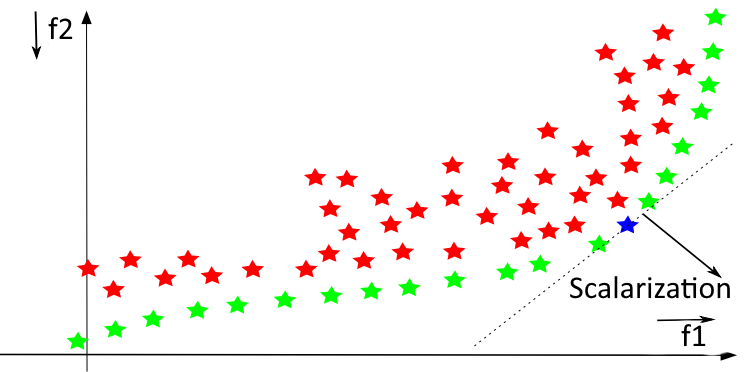
\includegraphics[scale=0.33]{3.png}
\end{center}
\columnbreak
\textbf{Budgeting}: bound the value of one of the losses\\
	$\min\{f_1(x)\:|\:f_2(x)\leq \beta_2,x\in X\}$, but which $\beta_2$?
\begin{center}
	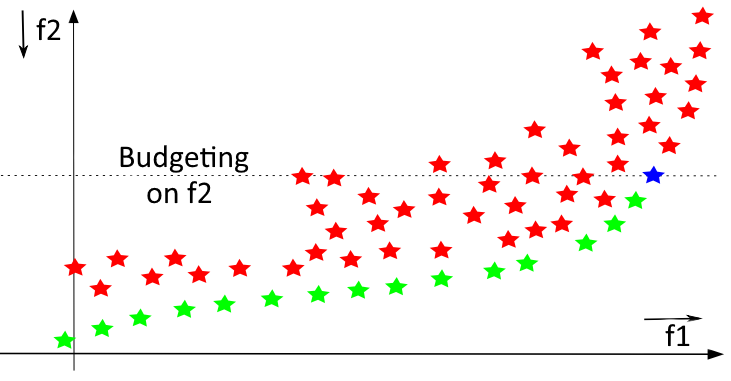
\includegraphics[scale=0.33]{4.png}
\end{center}
\end{multicols}
We will assume that this is done at modelling stage.
\subsection{Optimization is hard}
Even with single-objective, optimization is hard. It's impossible if $f$ has no minimum in $X$, for example $f(x) = x$: if $(P)$ is unbounded below, then $v(P) = -\infty$. Solving $(P)$ is actually at least two different things:
\begin{list}{}{}
	\item Finding $x_*$ and \textbf{proving $x_*$ it's optimal} (how?)
	\item Constructively \textbf{proving $f$ unbounded below} on $X$ (how?)
\end{list}
It's also impossible if $f_* > -\infty$ but $\not\exists\:x_*$, for example $f(x) = e^x$ or $f(x)=\left\{\begin{array}{l l}
1&\text{if }x = 0\\
|x|&\text{if }x \neq 0
\end{array}\right.$, but there are plenty of $\epsilon$-approximate solutions ($\epsilon$-optima) $$f(x_\epsilon)\leq f_* + \epsilon\:\:\:\:\forall\:\epsilon>0$$
and on computers $x\in \mathbb{R}$ is actually $x\in \mathbb{Q}$ with up to 16 digits precision, so approximation errors are unavoidable anyway. Exact algebraic computation is possible but too slow, so ML is actually going the opposite way (float, half, small integers\ldots). In short, \textbf{finding the exact $x_*$ is impossible in general}.
\paragraph{Optimization needs to be approximate} \begin{list}{}{}
	\item \textbf{Absolute gap} $$a_i = A(x_i) = f(x_i) - f_* \geq 0$$
	\item \textbf{Relative gap} $$r_i = R(x_i) = \frac{f(x_i) - f_*}{|f_*|} = \frac{A(x_i)}{|f_*|}\geq 0$$
\end{list}
The relative gap is useful because $\forall\:\alpha>0$ we have that $$(P)\equiv (P_\alpha) = \min\{\alpha f(x)\:|\:x\in X\}$$ and for the same $x_*$ we have $$v(P_\alpha) = \alpha v(P) \Rightarrow\text{same }R(x)\text{, different }A(x)$$\\
But in general computing the absolute/relative gap is hard because we don't know $f_*$, which is what we want to estimate. So it's hard to estimate how good a solution is. One could argue that this is the "issue" in optimization: compute an estimate of $f_*$.
\paragraph{Optimization is really hard} Impossible, even, because \textbf{isolated minima can be anywhere}, and restricting to $x\in X=[x_-, x_+]$ with $-\infty<x_-<x_+<+\infty$ doesn't help: still uncountable many points to try. Also $f$ can have isolated downward spike anywhere. Even on $X = [x_-, x_+]$ \textbf{the spikes can be arbitrarily narrow}.
\paragraph{Optimization at least possible} We \textbf{can impose $X=[x_-,x_+]$ with $D = x_+-x_-<\infty$}, meaning with a \textbf{fixed finite diameter}. We can also impose that the $f$'s spikes can't be arbitrarily narrow, so $f$ cannot change too fast $\Leftrightarrow$ $f$ Lipschitz continuous (L-c) on $X$: $$\exists\: L > 0\:|\:\forall x,y\in X\:\:\:|f(x) - f(y)| \leq L|x - y|$$
$f$ L-c $\Rightarrow$ doesn't "jump" and one $\epsilon$-optimum can be found with $O(\frac{L\cdot D}{\epsilon})$ evaluations by uniformly sampling $X$ with step $\frac{2\epsilon}{L}$. There's a bad news: no algorithm can work in less that $\Omega(\frac{L\cdot D}{\epsilon})$, but it's the worst case of $f$ (constant with one spike).\\
The number of steps is inversely proportional to accuracy: just not doable for small $\epsilon$. Dramatically worse with $X\subset R^n$.\\
Also generally $L$ is unknown and not easy to estimate, but algorithms actually require/use it.
\begin{list}{}{}
	\item $f$ \textbf{globally} L-c $\Leftrightarrow X=\mathbb{R}$
	\item $f$ \textbf{locally} L-c at $x \Leftrightarrow \exists\epsilon >0\:|\:X=[x-\epsilon,x+\epsilon]$
	\item Locally L-c at $x \not\Rightarrow$ globally L-c
	\item Locally L-c at $x \Rightarrow$ continuous at $x$
\end{list}
\subsection{Local Optimization} Even if I stumble in $x_*$ how do I recognize it? This is the difficult thing, which corresponds to knowing $f_*$. It's simpler to start with a weaker condition: $x_*$ is the \textbf{local minimum} if it solves $$\min\{f(x)\:|\:f\in X(x_*, \epsilon) = [x_* - \epsilon, x_* + \epsilon]\}$$ for some $\epsilon > 0$.\\
Stronger notion: \textbf{strict local minimum} if $$f(x_*) < f(y)\:\:\:\forall\:y\in X(x_*,\epsilon) - \{x_*\}$$
$f$ (strictly) \textbf{unimodal} on X if has minimum $x_* \in X$ and it is (strictly) decreasing on the left $[x_-, x_*]$ and (strictly) increasing on the right $[x_*, x_+]$. If $x_*$, then typically $\exists\:\epsilon>0\:|\:f$ is (strictly) unimodal on $X(x_*,\epsilon)$.\\
\textbf{Most functions are not unimodal, but they are if you focus on the attraction basin of $x_*$ and restrict there}. Unfortunately it's true for every local optima, and that's why they all look the same: all local optima are similar, including the global one, but this makes it finding some local optimum a lot easier. But finding the right one, the global optimum, is another matter entirely.
\begin{center}
	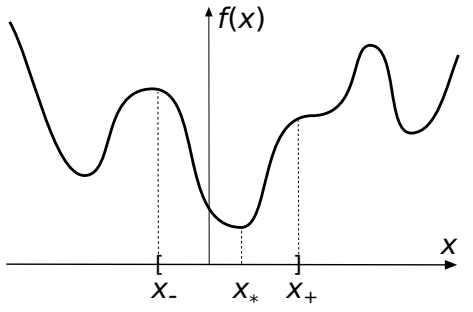
\includegraphics[scale=0.5]{5.png}
\end{center}
Once in the attraction basin, we can restrict it by evaluating $f$ in two points and excluding a part.
\begin{center}
	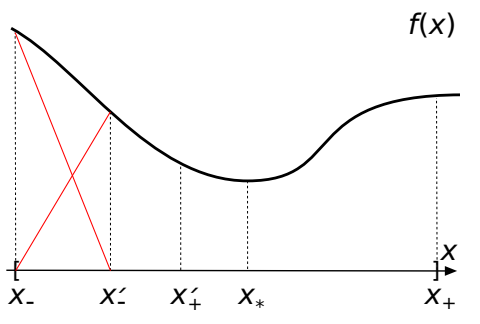
\includegraphics[scale=0.5]{6.png}
\end{center}
How to choose the part so that the algorithm go as fast as possible? Each iteration dumps the left or the right part, don't know which $\Rightarrow$ should be equal $\Rightarrow$ select $r \in (\frac{1}{2}, 1), x'_- = x'_- + (1 - r)D, x'_+ = x_- + rD$\\
Faster if $r$ larger $\Rightarrow$ $r = \frac{D}{2} + \epsilon = x'_\pm = x_- + \frac{D}{2} \pm \epsilon$ but next iteration will have two entirely different $x'_-, x'_+$ to evaluate $f$ on.
\paragraph{Optimally choosing the iterates} A generally powerful concept is to optimize the worst-case behavior $\Rightarrow$ shrink the intervals as quickly as possible.\\
Each iteration dumps either $[x_-, x_-']$ or $[x_+', x_+]$, we don't know which so they should be of equal size $\Rightarrow$ select $r\in (\frac{1}{2},1)$ so that $x_-' = x_- + (1-r)D$ and $x_+' = x_- + rD$\\
$r$ larger $\Rightarrow$ faster convergence, so $r = \frac{D}{2} + \epsilon \Leftrightarrow x_\pm' = x_- + \frac{D}{2}\pm\epsilon$ but next iteration will have two entirely different $x_-', x_+'$ to evaluate $f$ on.\\
So we actually want to \textbf{minimize function evaluations by reusing the surviving point}. $$r : 1 = (1 - r) : r \Leftrightarrow r\cdot r = 1 - r \Leftrightarrow r = \frac{\sqrt{5} - 1}{2} = 0.618 = \frac{1}{g}$$ with $g$ being the golden ratio, $g = \frac{\sqrt{5} + 1}{2} = 1.618 \Rightarrow g = 1 + r = 1 + \frac{1}{g}$\\
Theorems breed algorithms: \textbf{golden ratio search}\\
\begin{lstlisting}[style=myPython]
procedure x = GRS(f, xl, xr, delta)
	xl2 = xl + (1-r)(xr-xl)
	xr2 = xl + r(xr - xl)
	compute f(xl2), f(xr2)
	while (xr - xl > delta):
		if(f(xl2) > f (xr2))
			xl = xl2
			xl2 = x
			x = xr2
			xr2 = xl + r(xr - xl)
			compute f(xr2)
		else:
			xr = xr2
			xr2 = x
			x = xl2
			xl2 = xl + (1-r)(xr-xl)
			compute f(xl2)
\end{lstlisting}
After $k$ iterations, $x_+^k - x_-^k = Dr^k$ stops when $Dr^k \leq \delta$, so when $k = 2\log\frac{D}{\delta}$: exponentially faster, can work with small $\delta$.\\
Asymptotically optimal if no other information is available. $\delta \neq \epsilon$ but $f$ L-c $\Rightarrow A(x^k) \leq \epsilon$ when $k = 2\log\frac{LD}{\epsilon}$\\
First example of linear convergence $A(x^k) \leq Sr^k \leq \epsilon$ with $r < 1$, as fast as a negative exponential $\Rightarrow k \geq \frac{\displaystyle \log\frac{S}{\epsilon}}{\displaystyle \log\frac{1}{r}}$\\\\
$O(\log(\frac{1}{\epsilon}))$ is good, but the constant $\rightarrow\infty$ as $r\rightarrow 1$
\subsection{Faster Local Optimization}
\paragraph{To make it go faster, give it more information} Two points are needed to see in which direction $f$ is decreasing. If we could see this directly we could make it with one point, faster. Look at the linear function that best locally approximates $f$, trusty old first derivative $f'(x)$: slope of the tangent line to the graph of $f$ in $x$\\
First order model of $f$ at $x$: $$L_x(y)=f'(x)(y-x) + f(x)$$ $L_x(y) \simeq f(y)$ $\forall\:y\in[x-\epsilon, x+\epsilon]$ for some small $\epsilon > 0$.\\
$x_*$ local minimum $\Rightarrow f'(x_*) = 0 \Leftrightarrow$ root of $f' \Leftrightarrow$ stationary point. If $f'(x) < 0$ or $f'(x) > 0$, then $x$ is clearly not a local minimum. Hence, \textbf{$f'(x) = 0$ for the all local minima} (hence in the global minimum as well) but this is \textbf{true for the local maxima} (hence global maximum as well), as well in the plateau and saddle points. \textbf{To tell them apart, look at the second derivative $f''$}.
\begin{center}
	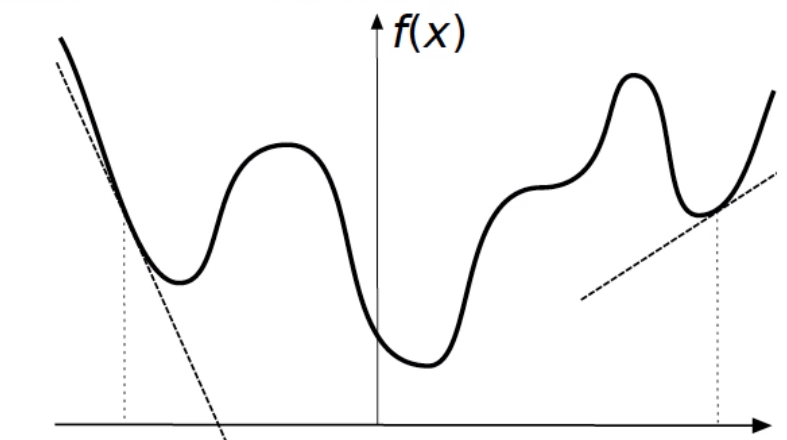
\includegraphics[scale=0.5]{1.png}
\end{center}
In simple cases we get the answer by a closed formula. In $f = bx + c$ linear, if $b > 0$ then the minimum is $x_-$ and maximum is $x_+$, viceversa if $b < 0$. For $f = ax^2 + bx + c$, quadratic, then if $a > 0$ the minimum is $\min\{ x_+, \max\{x_*, x_-\}\}$ and the maximum is $\arg\max\{f(x_-), f(x_+)\}$, and viceversa if $a < 0$.\\
Only polynomial whose roots have a closed formula (degree 3 and some degree 4), with basically no hope for most trascendental, trigonometric and mixed equations. We need an algorithm for solving non-linear equations.
\paragraph{Dichotomic Search} With $f'$ continuous, the \textbf{intermediate value theorem proves} that  $$f'(x_-) < 0 \wedge f'(x_+) > 0 \Rightarrow \exists\:x\in[x_-, x_+]\:|\: f'(x) = 0$$
Theorems breed algorithms $\rightarrow$ \textbf{Dichotomic Search}.
\begin{lstlisting}[style=myPython]
procedure x = DS(f, xl, xr, eps)
	while (true):  # invariant: df(xl)<-eps, df(xr)>eps
		x = in_middle_of(xl, xr)
		compute df(x)
		if (abs(df(x)) <= eps): break
		if (df(x) < 0):
			xl = x
		else:
			xr = x
\end{lstlisting}
With \texttt{df} meaning $f'$\\
For \texttt{in\_middle\_of(xl, xr)} the obvious choice is \texttt{return (xl + xr)/2;}. We have linear convergence with $\gamma = 0.5 < 0.618 \Rightarrow k = 1.45\log(\frac{LD}{\epsilon}) < 2 \log(\frac{LD}{\epsilon})$\\
The condition $f'(x_-) < -\epsilon, f'(x_+) > \epsilon$ is important. If this is not satisfied, we move the interval more and more to the right until the derivative is possible.
\begin{lstlisting}[style=myPython]
delta_x = 1  # or whatever value > 0
while (df(r) <= -eps):
	xr = xr + delta_x
	delta_x = 2 * delta_x  # or whatever factor > 1
\end{lstlisting}
The same in reverse of $x_-$ with $\Delta x = -1$. This works in practice for all "reasonable" functions. Works if $f$ coercive ($\lim_{|x| \to \infty} f(x) = \infty$)\\
The definition of derivative is
$$f'(x) = \lim_{t\to 0} \frac{f(x+t)-f(x)}{t}$$
Provided that the limit is finite and that it exists at all, and given the left and right derivatives
$$f'_-(x) = \lim_{t\to 0_-} \frac{f(x+t)-f(x)}{t}$$
$$f'_+(x) = \lim_{t\to 0_+} \frac{f(x+t)-f(x)}{t}$$
We say that $f$ is \textbf{differentiable} at $x$ $\Leftrightarrow f'(x)$ exists $\Leftrightarrow f'_-(x)=f'_+(x)$ both finite.\\
There exists easy closed-forms for most functions (with notable exceptions such as $\max\{\}$). Also, $f$ differentiable in $x \Rightarrow f$ continuous in $x$ (but the opposite is not true).
\begin{list}{}{}
	\item $f' \in C^0 \Leftrightarrow f \in C^1 \Leftrightarrow$ continuously differentiable $\Rightarrow f\in C^0$
	\item $f'' \in C^0 \Leftrightarrow f\in C^2 \Leftrightarrow f' \in C^1 \Rightarrow f' \in C^0 \Rightarrow f \in C^1 \Rightarrow f \in C^0$
	\item $f \in C^1$ globally L-c on $X \Rightarrow |f'(x)| \leq L\:\:\forall\: x \in X$
\end{list}
\paragraph{Extreme value theorem} $f \in C^0$ on $X = [x_-, x_+]$ finite $\Rightarrow$ max$\{f(x)\:|\: x\in X\} < \infty$, min$\{f(x)\:|\: x\in X\} > -\infty$\\\\
$f\in C^1$ on $X$ finite $\Rightarrow f$ globally L-c on $X$\\
Best possible case is $f\in C^2$ on finite $X\Rightarrow$ both $f$ and $f'$ globally L-c on $X$
\paragraph{Fastest local optimization} Interpolation, for improving the dichotomic search. Choosing $x$ "right in the middle" is the dumbest possible approach, because we know a lot about $f$: $f(x_-), f(x_+), f'(x_-), f'(x_+)\ldots$. So let's use that, by constructing a model of $f$ based on known information. Much better choosing $x$ close to $x_*$.\\
But remember that \textbf{the model is an estimate}, so never completely trust the model, but regularize, stabilize\ldots in this case, the minimum guaranteed decrease is with $\sigma < 0.5$, and the worst case is linear convergence with $r = 1 - \sigma$, but hopefully is much faster than that when the model is "right".
\subsection{Measuring algorithms speed} Given the sequences \begin{list}{}{}
	\item Iterates: $\{x_i\}$
	\item Distances from $x_*$: $\{d_i = |x_i - x_*|\}$
	\item $f$-values: $\{f_i = f(x_i)\}$
	\item Absolute gaps: $\{a_i = A(x_i) = f(x_i) - f_*\}$
	\item Relative gaps: $\{r_i = R(x_i) = \frac{f(x_i) - f(x)}{|f_*|} ) \frac{A(x_i)}{|f_*|}\}$
\end{list}
We have convergence when $\{a_i\} \rightarrow 0, \{r_i\} \rightarrow 0 \Leftarrow \{d_i\} \rightarrow 0$ (but $\not\Rightarrow)$, but how rapidly? \textbf{Rate of convergence}
$$\lim_{i\to\infty} \left(\frac{f_{i+1} - f_*}{f_i - f_*}\right)^p = \lim_{i\to\infty} \left(\frac{a_{i+1}}{a_i}\right)^p = \lim_{i\to\infty} \left(\frac{r_{i+1}}{r_i}\right)^p = r$$
\begin{list}{}{}
	\item[$p = 1$]\begin{list}{}{}
		\item $r = 1\Rightarrow$ \textbf{sublinear} \begin{list}{}{}
			\item $\frac{1}{i} \Rightarrow k \in O(\frac{1}{\epsilon})$ (bad)
			\item $\frac{1}{i^2} \Rightarrow k \in O(\frac{1}{\sqrt{\epsilon}})$ (a bit better)
			\item $\frac{1}{\sqrt{i}} \Rightarrow k \in O(\frac{1}{\epsilon^2})$ (horrible)
		\end{list}
		\item $r = 0\Rightarrow$ \textbf{superlinear}
		\item $r < 1\Rightarrow$ \textbf{linear}, $r_i \rightarrow i \in O(\log(\frac{1}{\epsilon}))$, good unless $r = 1$
	\end{list}
	\item[$p = 2$]\begin{list}{}{}
		\item $r > 0\Rightarrow$ \textbf{quadratic}, best we can reasonably hope for\\
	$\frac{1}{2^{2^i}} \Rightarrow i \in O(\log(\log(\frac{1}{\epsilon})))$, which is basically $O(1)$: the number of correct digits doubles at each iteration
	\end{list}
\end{list}
\paragraph{Improving dichotomic search} Quadratic interpolation has superlinear convergence if started "close enough".\\
$$f\in C^3, f'(x_*) = 0 \wedge f''(x_*)\neq 0 \Rightarrow \exists\:\delta > 0\:|\:x_0 \in [x_* - \delta, x_* + \delta] \Rightarrow \{x_i\} \rightarrow x_*$$ with $p = \frac{1 + \sqrt{5}}{2}$ exponent of superlinear convergence, and $x_0$ the starting point of the algorithm.\\\\
Four conditions $\Rightarrow$ can fit a cubic polynomial and use its minima. Theoretically pays: quadratic convergence ($p = 2$) and seems to work well in practice.
\paragraph{Newton's method} More derivatives, so same information with less points. First order model of $f'$ at $x_i$ $$L_i'(x) = L_{x_i}'(x) = f'(x_i) + f''(x_i)(x-x_i)\simeq f'(x)$$ and solve $L'_i(x) = 0 \simeq f'(x) = 0 \Rightarrow x = x_i-\frac{f'(x_i)}{f''(x_i)}$
\begin{lstlisting}[style=myPython]
procedure x = NM(f, x, eps)
	while (abs(df(x)) > eps):
		x = x - (df(x)/ddf(x))
\end{lstlisting}
With \texttt{df} meaning $f'$ and \texttt{ddf} meaning $f''$.\\
Alternatively construct a second order model $$Q_i(x) = Q_{x^i}(x) = f(x^i) + f'(x^i)(x - x^i) + f''(x^i)\frac{(x - x^i)^2}{2}$$ and then minimize it.\\\\
Numerically delicate: what if $f''(x) \simeq 0$? Converges (at all) only if started close enough to $x_*$.\\
If we get within a short enough distance $\delta$, then it will converges extremely fast with $p = 2$. Mathematically, $f\in C^3, f'(x_*) = 0 \wedge f''(x_*)\neq 0\Rightarrow \exists\:\delta>0\:|\:x_0\in[x_*-\delta, x_*+\delta]\Rightarrow \{x_i\} \rightarrow x_*$ with $p = 2$.
\pagebreak
\subsection{Global optimization} Unless strong assumptions are made, we can't say much about global optimization.\\
The obvious one would be unimodal, but not easy to verify/construct. Workable alternative: $f$ convex ($\Rightarrow$ unimodal).
\paragraph{Convexity} Convex means that $f'$ monotone non decreasing and $f'' \geq 0$. But convexity $\not\Rightarrow C^1$. Some functions are convex and a few operators preserve convexity. Many models are purposely constructed convex $\Rightarrow$  \textbf{Spatial Branch-and-Bound approach}: sift through all $X = [x_-, x_+]$ using clever guide, convex lower approximation \underline{$f$} of nonconvex $f$ on $X$.
\begin{center}
	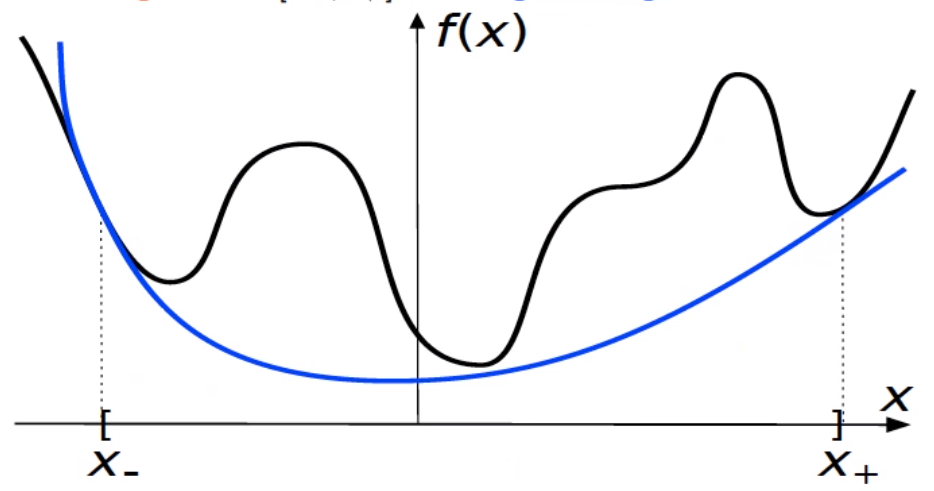
\includegraphics[scale=0.5]{2.png}
\end{center}
"Easily" find local $\Leftrightarrow$ global minimum $\tilde{x}$ giving \underline{$f$}$(\tilde{x}) \leq f_* \leq f(\tilde{x})$. If the gap $f(\tilde{x}) - \underline{f}(\tilde{x})$ is too large, we partition $X$ and iterate. If on some partition $\underline{f}(\tilde{x}) \geq$ best $f$-value so far, then that partition is killed.\\
In the worst case, exponential complexity because you keep dicing and slicing $X$. But it is exponential in practice too. It depends on how much non-convex $f$ is and how good of a lower approximation $\underline{f}$ is. A cleverer approach is carefully choosing the non-convexities.
%end 1-first steps.pdf
\section{Unconstrained optimization}
From now on we'll use $$f:\mathbb{R}^n\rightarrow \mathbb{R}$$ $$f(x_1,x_2,\ldots,x_n) = f(x)$$ $$x = [x_i]_{i=1}^n = [x_1,\ldots,x_n]\in \mathbb{R}^n$$
Note that $\mathbb{R}^n = \mathbb{R}\times \mathbb{R} \times\ldots\times \mathbb{R}$, which is \textbf{exponentially larger} than $\mathbb{R}$.\\
$I = [x_-, x_+], X = I\times I \times\ldots\times I$ hypercube (or hyperrectangle if intervals are disequal). A lot more space to look at, meaning much more difficult task.\\
We need $f$ to be L-c, and sadly no algorithm can work in less than $$\Omega\left(\left(\frac{LD}{\epsilon}\right)^n\right)$$
Recall that $L$ comes from the L-c property
$$\exists\:L>0\:|\:\:|f(x)-f(y)\leq L|x-y|$$
and $D$ comes from the diameter of the interval, e.g. with $X=[x_-,x_+]$ we have
$$D=x_+-x_- < \infty$$
\textbf{Curse of dimensionality}: not really doable unless $n = 3, 5, 10$ tops. Can make to $O\left(\left(\frac{LD}{\epsilon}\right)^n\right)$, with multidimensional grid and small enough step (standard approach to hyperparameter optimization). If $f$ analytic, clever B\&B can give global optimum. If $f$ black-box (typically, no derivatives), many heuristics can give good solutions, probably not optimal.
\paragraph{Unconstraint global optimization} If $f$ is convex, then global $\Leftrightarrow$ local which is much better: most (but not all) convergence results are dimension independent and if there's dependence it is not exponential. Doesn't mean that all local algorithms are fast: speed may be low (badly linear), cost of $f$ or derivatives computation increases with $n$ dimension (for large n even $O(n^2)$ may be too much) and some dependency on $n$ may be hidden in $O(\:)$ constraints. Yet, large scale optimization can be done.
\paragraph{Notation}\begin{list}{}{}
	\item \textbf{Scalar product} $\langle x,y\rangle = x^Ty = \sum_{i=1}^n x_iy_i = x_1y_1+\ldots+x_ny_n$
	\item \textbf{Norm} $\|x\| = \sqrt{x_1^2+\ldots+x_n^2} = \sqrt{\langle x,x\rangle}$
	\item \textbf{Distance} $d(x,y) = \|x-y\| = \sqrt{(x_1-y_1)^2+\ldots+(x_n-y_n)^2}$
	\item \textbf{Ball} with center $x\in \mathbb{R}^n$ and radius $r > 0$ is $B(x,r) = \{y\in \mathbb{R}^n\:|\:\|y-x\|\leq r\}$
\end{list}
Usually $f:D\rightarrow \mathbb{R}$ with $D = dom(f)$ domain of $f$ which may not be all $\mathbb{R}^n$, but usually ok to ignore $dom(f)$ and assume $f(x)=\infty$ for $x\not\in D$
\begin{list}{}{}
	\item \textbf{Graph} of $f$ lives in $\mathbb{R}^{n+1}$: $gr(f) = \{(f(x),x)\:|\:x\in \mathbb{R}^n\}$
	\item \textbf{Epigraph} of $f$ lives in $\mathbb{R}^{n+1}$: $epi(f)=\{(v,x) \in \mathbb{R}^{n+1}\:|\:v\geq f(x)\}$
	\item \textbf{Level set} at value $v$: $L(f,v)=\{x\in \mathbb{R}^n\:|\:f(x)=v\}$
	\item \textbf{Sublevel set} at value $v$: $S(f,v)=\{x\in \mathbb{R}^n\:|\:f(x)\leq v\}$
\end{list}
We have that $x_* \in S(f,v)\:\:\:\forall\:v\geq f_*$ and $S(f,v) = \emptyset\:\:\:\forall\:v<f_*$

\paragraph{Tomography} $f:\mathbb{R}^n \rightarrow \mathbb{R}$ with $x\in \mathbb{R}^n$ origin and $d\in \mathbb{R}^n$ direction. You can define $\phi_{x,d}(\alpha) = f(x + \alpha d): \mathbb{R} \rightarrow \mathbb{R}$ \textbf{tomography} of $f$ from $x$ along $d$.\\
$\phi_{x,d}$ can always be pictured, but there are infinitely many of them: which $x,d$?\begin{list}{}{}
	\item $\|d\|$ only changes the scale: $\phi_{x,\beta d}(\alpha) = \phi_{x,d}(\beta \alpha)$ so often convenient to use normalised direction ($\|d\| = 1$)
	\item Simplest case: restriction along $i$-th coordinate\\
	$f_x^i(\alpha) = f(x_1,\ldots,x_{i-1},\alpha,x_{i+1},\ldots,x_n) = \phi_{0,u^i}(\alpha)$ with $\|u^i\| = 1$
	\item When $x,d$ clear from context, then $\phi(\alpha)$
\end{list}
\paragraph{Simple Functions} \begin{list}{}{}
	\item \textbf{Linear} $b \in \mathbb{R}^n, c\in \mathbb{R}$ $$f(x) = \langle b,x\rangle + c$$
	Tomography $f(x) = \langle b,x\rangle, x = 0, \|d\|=1$: $\phi(\alpha) = \alpha\langle b, d\rangle = \alpha\|b\|\cos(\theta)$\\
	Plotting this gives a line, increasing because "$b$ same direction as $d$", more collinear $\Rightarrow$ steeper. Collinear means steepest line, less collinear means less steap. 90° angle means a flat line. Decreasing if opposite directions.\\
	$\min f(x)$ when $\not\exists\:x_*$ if $b \neq 0$ ($\Rightarrow \exists\: d\:|\:\langle b,d\rangle \neq 0$), $\forall\:x$ if $b = 0$
	\item \textbf{Quadratic} with fixed $Q\in \mathbb{R}^{n\times n}, q\in \mathbb{R}^n$ we have $$f(x) = \frac{1}{2}x^TQx + qx$$
	If $q=0$ (no linear term), then \textbf{homogeneous quadratic}.\\
	Tomography $\phi(\alpha) = f(\alpha d) = \alpha^2(d^TQd)\Rightarrow$ sign and steepness depend on $d^TQd$, so we need to know about signs of $d^TQd$. Steeper when $d$ along one axe, least steep when $d$ along the other axe and intermediate steepness when "in between". Again, steeper along the opposite of one axe and least steep along the opposite of the other axe.\\
	With $q\neq 0$ but $Q$ nonsingular then $\lambda_i\neq 0\:\:\:\forall\:i$, then $f(x)=\frac{1}{2}(x-x_*)^TQ(x-x_*) [+c]$ for $x_* = -Q^{-1}q$ and $x_* \neq 0$ center of the level sets (which shapes are determined by the eigenvalues).\\
	$y = x - x_*, f_*(y) = y^TQy [+c]$
\end{list}
\paragraph{Directional/partial derivatives} The directional derivative of $f:\mathbb{R}^n\rightarrow \mathbb{R}$ at $x\in \mathbb{R}^n$ along the direction $d\in \mathbb{R}^n$ is $$\frac{\partial f}{\partial d}(x) = \lim_{t\to 0}\frac{f(x+td) - f(x)}{t} = \phi_{x,d}'(0)$$
How can $\phi_{x,d}'(0)$, the derivative of the $(x,d)$-tomography (in 0), be computed? A special case is $\frac{\partial f}{\partial x_i}(x)$, partial derivative of $f$ with respect to $x_i$ at $x\in \mathbb{R}^n$, easy to compute by just treating $x_j$ for $j\neq i$ as constants.\\
The \textbf{gradient} is the column vector of all partial derivatives $$\nabla f(x) = \left[\begin{array}{c}
\frac{\partial f}{\partial x_1}(x)\\
\vdots\\
\frac{\partial f}{\partial x_n}(x)
\end{array}\right]$$
$$f(x) = \langle b,x\rangle \Rightarrow\nabla f(x) = b$$
$$f(x) = \frac{1}{2}x^TQx + qx \Rightarrow\nabla f(x) = Qx + q$$
$f$ differentiable at $x$ if $\exists$ linear function $\psi(h) =\langle b,h\rangle + f(x)$ such that $$\lim_{\|h\|\to 0}\frac{|f(x+h) - \psi(h)|}{\|h\|} = 0$$ $$\Rightarrow \psi(0) = f(x) \Rightarrow c = f(x)$$
$\psi$ is equivalent to the first order model of $f$ at $x$, the error of this equivalence vanishes faster than linearity. So $f$ differentiable at $x\Rightarrow b = \nabla f(x)$ and\begin{list}{}{}
	\item $\Rightarrow \frac{\partial f}{\partial x_i}(x)$ exists for every $i$ (but $\Leftrightarrow$ not true)
	\item $\Rightarrow$ first order model of $f$ at $x$ is $L_x(y) = \nabla f(x)(y-x)$
\end{list}
$f$ differentiable $\Rightarrow$ all relevant objects in $\mathbb{R}^{n+1}$ and $\mathbb{R}^n$ are smooth. If $f$ is non differentiable $\Rightarrow$ kinks appear and things break,
\paragraph{Jacobian} Given a vector-valued function $f:\mathbb{R}^n\rightarrow \mathbb{R}^m$, $f(x) = [f_1(x), f_2(x),\ldots,f_m(x)]$, the partial derivatives are the same with extra index $$\frac{\partial f_j}{\partial x_i}(x) = \lim_{t\rightarrow 0}\frac{f_j(x_1,\ldots,x_{i-1},x_i+t,x_{i+1},\ldots,x_n) - f_j(x)}{t}$$
The \textbf{Jacobian} is the matrix of all $n\cdot m$ partial derivatives
$$Jf(X) = \left[ \begin{array}{c c c}
\frac{\partial f_1}{\partial x_1}(x) & \ldots & \frac{\partial f_1}{\partial x_n}(x)\\
\vdots&\ddots&\vdots\\
\frac{\partial f_m}{\partial x_1}(x) & \ldots & \frac{\partial f_m}{\partial x_n}(x)\\
\end{array}\right] = \left[\begin{array}{c}
\nabla f_1(x)^T\\\vdots\\\nabla f_m(x)^T
\end{array}\right]$$
A $n\times m$ matrix with gradients as rows.
\paragraph{Hessian} The $\frac{\partial f}{\partial x_i}:\mathbb{R}^n\rightarrow \mathbb{R}$ have partial derivatives themselves. \textbf{Second order partial derivative}, just do it twice $$\frac{\partial^2 f}{\partial x_i \partial x_j}$$ $$\frac{\partial^2 f}{\partial x_i \partial x_i}=\frac{\partial^2 f}{\partial x_i^2}$$
So $\nabla f(x) : \mathbb{R}^n \rightarrow \mathbb{R}^n$ have a Jacobian and it's called \textbf{Hessian} of $f$ at $x$
$$\nabla^2 f(x) = J\nabla f(x) = \left[ \begin{array}{c c c c}
\frac{\partial^2 f}{\partial x_1^2}(x) & \frac{\partial^2 f}{\partial x_2\partial x_1} & \ldots & \frac{\partial^2 f}{\partial x_n\partial x_1}(x)\\
\vdots&\ddots&\ddots&\vdots\\
\frac{\partial^2 f}{\partial x_1\partial x_n}(x) & \frac{\partial^2 f}{\partial x_2\partial x_n}(x) & \ldots & \frac{\partial^2 f}{\partial x_n^2}(x)\\
\end{array}\right]$$
Requires $O(n^2)$ to store and at least $O(n^2)$ to compute, unless sparse.\\
$f(x) = \frac{1}{2}x^TQx + qx \Rightarrow \nabla^2 f(x) = Q$\\
Second order model = first order model plus second order term (better)
$$Q_x(y) = L_x(y) + \frac{1}{2}(y-x)^T\nabla^2f(x)(y-x)$$
\subparagraph{Theorem} $\exists\:\delta>0\:|\:\forall\:y\in B(x, \delta)$ we have that $\frac{\partial^2 f}{\partial x_j\partial x_i}(y)$ and $\frac{\partial^2 f}{\partial x_i\partial x_j}(y)$ exist and are continuous in $x$\begin{list}{}{}
	\item $\Rightarrow \frac{\partial^2 f}{\partial x_j\partial x_i}(y) = \frac{\partial^2 f}{\partial x_i\partial x_j}(y) \Leftrightarrow \nabla^2 f$ symmetric
	\item $\Rightarrow$ all eigenvalues of $\nabla^2 f(x)$ are real
\end{list}
With $f\in C^2$ we have $\nabla^2 f(x)$ continuous everywhere, so symmetric everywhere. $C^2$ is the best class for optimization.
\subsection{Optimality conditions}
$f$ differentiable at $x$ and $x$ local minimum $\Rightarrow \nabla f(x) = 0 \Leftrightarrow$ stationary point ($\not\Leftarrow$): to tell them apart we need to look at the curvature of $f$. If $f$ quadratic I would know, looking at the eigenvalues of $Q = \nabla^2 f(x)$, so we could approximate $f$ with a quadratic function: the second order model $$Q_x(y) = L_x(y) + \frac{1}{2}(y-x)^T\nabla^2f(x)(y-x)$$
$$\nabla Q_x(x) = \nabla L_x(x) = \nabla f(x) \Rightarrow \nabla Q_x(x) = 0$$otherwise not minimum. Meaning that in a local minimum there cannot be directions of negative curvature, $\nabla^2 f(x) \geq 0 \Leftrightarrow x$ (global) minimum of $Q_x$. Requires the second-order Taylor's theorem
$$f(y) = L_x(y) + \frac{1}{2}(y-x)^T\nabla^2 f(x)(y-x) + R(y-x)$$
Another condition necessary and almost sufficient: $f\in C^2$, $\nabla f(x) = 0$ and $\nabla^2f(x)\succ 0\Rightarrow x$ local minimum. Avoids the bad case $d^T\nabla^2f(x)d=0$ meaning zero curvature direction.
\subsection{Convex functions}
$f$ convex $\Leftrightarrow \forall\:x,y\in\mathbb{R}^n\:\alpha\in [0,1]$
$$\alpha f(x) + (1-\alpha)f(y)\geq f(\alpha x+(1-\alpha)y)$$
$f$ concave $\Leftrightarrow -f$ convex.\\
$f\in C^1$ convex $\Leftrightarrow\nabla f$ monotone $\Leftrightarrow L_x(y) = f(x)+\langle\nabla f(x), y-x\rangle\leq f(y)$
\begin{list}{}{}
	\item $f\in C^1$ convex: $\nabla f(x) = 0\Leftrightarrow x$ global minimum
	\item $f\in C^2$: $f$ convex $\Leftrightarrow\forall\:x\in\mathbb{R}^n \nabla^2 f(x)\succeq 0$
	\item $f\in C^2$ with $\nabla^2 f\succ 0$ absolutely the \textbf{best case} for optimization
\end{list}
%end 2-uncostrained optimality.pdf
\subsection{Gradient Methods}
\paragraph{Multivariate optimization algorithms} These are \textbf{iterative} procedures: start from an initial guess $x_0$ and compute some process $x_i \longrightarrow x_{i+1}$ to get a \textbf{sequence} $\{x_i\}$ that \textbf{\textit{should} go towards an optimal solution}.\\
$\{x_i\}\rightarrow x_*$ is one option, the best one, but not the only possibility.\\
At least $\{f_i = f(x_i)\} \rightarrow f_*$: \textbf{minimizing sequence}, and clearly $\{x_i\}\rightarrow x_* \Rightarrow \{f_i\}$ minimizing sequence, but $\not\Leftarrow$\\
Two general forms of the process $x_{i+1} = x_i + \alpha_id_i$:
\begin{list}{}{}
	\item \textbf{Line search}: first choose $d_i\in \mathbb{R}^n$ (\textbf{direction}), then choose $\alpha_i\in \mathbb{R}$ (\textbf{step size} $\Leftrightarrow$ learning rate in ML)
	\item \textbf{Trust region}: first choose $\alpha_i\in \mathbb{R}$ (\textbf{trust radius}), then $d_i\in \mathbb{R}^n$
\end{list}
The crucial concept is that the \textbf{model} $f_i \simeq f$ is used to construct $x_{i+1}$ from $x_i$
\paragraph{Compactness}
With $\{n^i\}\subset\{1,2,3,\ldots\}$ we have the \textbf{subsequence} $\{x^{n^i}\}\subseteq\{x^i\}$\\
$x$ is an \textbf{accumulation point} of $\{x^i\}$ if $\exists\:\{x^{n^i}\}\rightarrow x$\\
$X\subseteq\mathbb{R}^n$ is \textbf{closed} if $\forall\:\{x^i\}\subset X$ we have $\{x^i\}\rightarrow x\Rightarrow x\in X$\\
$X\subseteq\mathbb{R}^n$ is \textbf{bounded} if $\exists\:r>0\:|\:X\subseteq B(0,r)$\\
If $X\subseteq\mathbb{R}^n$ is closed and bounded, then it's \textbf{compact} (\textbf{Bolzano-Weierstrass Theorem}), which means $\{x^i\}\subset X\Rightarrow\exists$ accumulation point of $\{x^i\}$.
\paragraph{First order model $\Leftrightarrow$ gradient method} The first order model is the simplest model $$L_i(x) = L_{x_i}(x) = f(x_i) + \nabla f(x_i)(x-x_i)$$ Idea: $x_{i+1} \in \arg\min\{L_i(x)\:|\:x\in \mathbb{R}^n\} = \emptyset$, $L_i$ unbounded below on $\mathbb{R}^n$\\
It shouldn't move too far from $x_i$, $L_i$ is only "good" as $\alpha_i\rightarrow 0 \Rightarrow d_i = \arg\min\left\{\lim_{t\to 0} \frac{f(x+td)}{t}\right\} = -\nabla f(x_i) =$ steepest descent direction.\\
$\frac{\partial f}{\partial d_i}(x_i) < 0$ but $\frac{\partial f}{\partial d_i}(x_i + \alpha d_i)$ likely $> 0$ when $\alpha$ grows $\Rightarrow f$ grows instead of decreasing $\Rightarrow$ very long steps are bad unless $f_* = -\infty$. Very short steps are bad too: $f$ decreases, but very slowly.
\paragraph{Step selection} The issue is to find the \textbf{Goldilocks Step} $\alpha_i$ efficiently (a few function evaluations). Two extreme strategies:
\begin{list}{}{}
	\item \textbf{Fixed Stepsize} (FS): $\forall\:i\:\:\:\alpha_i = \tilde{\alpha}$ (how is chosen?)\\
	Most inexpensive.
	\item \textbf{(Exact) Line Search} (LS): $\alpha_i\in \arg\min\{f(x_i+\alpha d_i)\:|\:\alpha\geq 0\}$\\
	Most expensive but may converge faster.
\end{list}
Of course, something in the middle is better. $\phi'_i$ low-degree polynomial
$$\phi_i(\alpha) = f(x_i+\alpha d_i) = \phi_{x_i,d_i}(\alpha)$$
\paragraph{Gradient for quadratic functions} $f(x) = \frac{1}{2}x^TQx + qx$ with $Q\succeq 0$ otherwise $f$ is unbounded below. $x_*$ solves $Qx = -q$ if it exists, which is linear algebra but the linear system requires at most $O(n^3)$ while computing $d_i = -\nabla f(x_i) = -Qx_i - q$ is $O(n^2)$\\
Line search is easy, $O(n^2)$ with $\alpha_i = \frac{\|d_i\|^2}{d_i^TQd_i}$
\begin{lstlisting}[style=myPython]
procedure x = SDQ(Q, q, x, eps):
	while (||nablf(x)||>eps):
		d = -nablf(x)
		alpha = ||d||^2/dT*Q*d
		x = x + alpha*d
\end{lstlisting}
With \texttt{nablf} being $\nabla f$
\subparagraph{Analysis} Never obvious because we have to use properties of $x_*$ which is unknown, but in this case there's a nifty trick
$$f_*(x) = \frac{1}{2}(x-x_*)^TQ(x-x_*) = f(x) - f_*(x) = A(x)$$
for which, with $Q$ positive definite $$A(x_{i+1}) = \left(1-\frac{\|d_i\|^4}{(d_i^TQd_i)(d_i^TQ^{-1}d_i)} \right)A(x_i)$$
This becomes linear convergences ($\lambda_1,\lambda_{n}$ being respectively the max and min eigenvalues of $Q$)
\begin{list}{}{}
	\item Simple $A(x_{i+1}) \leq (1-\frac{\lambda_n}{\lambda_1})A(x_i)$
	\item Elaborated $A(x_{i+1}) \leq \frac{\lambda_1 - \lambda_n}{(\lambda_1 - \lambda_n)^2}A(x_i)$
\end{list}
The good news is that $n$ doesn't appear, it's \textbf{dimension-independent} so doable for very large scale machine learning. The bad news is that the rate of convergence $r\rightarrow 1$ as conditioning of $Q = \frac{\lambda_1}{\lambda_n}\rightarrow\infty$
\paragraph{When linear convergence may not be enough} The convergence is fast if $\lambda_1\simeq \lambda_n$ (one iteration for $\|x\|^2$) and rather slow if $\lambda_1 >> \lambda_n$. Intuitively, the algorithm zig-zags a lot when level sets are very elongated. Another bad news is that there may be an "hidden dependency": $\lambda_1$ and $\lambda_n$ may depend on $n$ and $\frac{\lambda_1}{\lambda_n}$ may grow as $n\rightarrow\infty$.\\
Let's extend it to every function.
\subsubsection{Gradient methods for general functions}
Given $f$ a general nonlinear function, the algorithm is almost the same:
\begin{lstlisting}[style=myPython]
procedure x = SDQ(f, x, eps):
	while (||nablf(x)||>eps):
		d = -nablf(x)
		alpha = stepsize(f, x, d)
		x = x + alpha*d
\end{lstlisting}
\texttt{stepsize} is the crucial part: FS or (inexact) LS. Need to avoid two opposite problems:
\begin{list}{}{}
	\item \textbf{Scylla}: $\alpha_i$ not too large to avoid $f(x_{i+1}) > f(x_i)$
	\item \textbf{Charybdis}: $\alpha_i$ not too small to avoid stalling
\end{list}
With $\frac{\partial f}{\partial d_i}(x_i)<0$ hence $\alpha_i\rightarrow 0$ we avoid Scylla but may hit Charybdis.\\
\texttt{stepsize(f, x, d)} $= LS(\phi_{x,d}, [0,\infty], \epsilon')$ is attractive but $\epsilon' = 0$ in general is not possible: how to choose it? Depends on the stopping criterion in $LS()$, let's assume $|\phi_{x,d}(\alpha)| \leq \epsilon'$. A fundamental property is $$\phi'_i(\alpha) = \frac{\partial f}{\partial d_i}(x_i + \alpha d_i) = \langle\nabla f(x_i+\alpha d_i), d_i\rangle$$
$$\Rightarrow |\phi_i'(\alpha_i)| = |\langle d_i, \nabla f(x_{i+1})\rangle| = |\langle \nabla f(x_i),\nabla f(x_{i+1})\rangle|$$
The good news is that only an approximate stationary point of $\phi_i$ is needed, not a global minimum (and not even a local minimum, can be a local maximum or a saddle point) $\Rightarrow f$ convex/unimodal is not needed. Also we can prove that the algorithm works with $\epsilon' = \epsilon \|\nabla f(x_i)\|$\\
A bad news is that the LS should become more accurate as the algorithm proceeds, although the LS can be very approximate ("far from $x_*$").\\
Usually works well in practice with arbitrary fixed $\epsilon'$
\paragraph{Notes on the stopping criterion} One would want $A(x_i)<\epsilon$ or $R(x_i) < \epsilon$ as stopping criterion, the issue is that $f_*$ is often unknown and cannot be used online. We need a lower bound $\underline{f} \leq f_*$, tight at least towards termination, but in general there are no good $\underline{f}$ available because good estimates of $f_*$ are hard to get.\\
We can use $\|\nabla f(x_i)\|$ as proxy of $A(x_i)$ (small $\Rightarrow$ small) but the exact relationship is hard to assess, so choosing $\epsilon$ is not obvious.\\
Sometimes we use a relative stopping condition $\|\nabla f(x_i)\|\leq \epsilon\|\nabla f(x_0)\|$, and sometimes $\|\nabla f\|$ has some meaning that can be used. Sometimes, we don't really care if $A(x_i)$ or $R(x_i)$ are small (machine learning).
\paragraph{Efficiency} The efficiency is basically the same.\\
With $f\in C^2, x_*$ local minimum such that $\nabla^2f(x_*)$ positive definite, exact LS $\{x_i\}\rightarrow x_* \Rightarrow \{f_i\}_{i\geq k}\rightarrow f_*$ linearly for large enough $k$, with $r = \frac{\lambda_1 - \lambda_n}{\lambda_1 + \lambda_n}^2$ with $\lambda_1,\lambda_n$ those of $\nabla^2 f(x_*)$\\
The result can be extended to inexact LS with $r\simeq 1-\frac{\lambda_n}{\lambda_1}$ (worse), with "$\simeq$" depending on LS parameters.
\subsubsection{Fixed Stepsize}
With $\alpha_i = \tilde{\alpha}$ for each $i$ it's much simpler but also rigid. Easier to avoid Charybdis: $\sum_{i=1}^\infty \alpha_i = \infty$\\
Yet $d_i = -\nabla f(x_i) \Rightarrow$ one wants $\{\|d_i\|\}\rightarrow 0$, so care is still required. We also have that $\alpha_i\rightarrow 0$ surely avoid Scylla, but it's not possible here.\\
The fundamental trick is $d_i = -\nabla f(x_i) \Rightarrow \|x_{i+1} - x_i\|$ automatically changes along iterations even if $\alpha_i$ is fixed.\\
$d_i = \frac{-\nabla f(x_i)}{\|\nabla f(x_i)\|} \Leftrightarrow \|d_i\| = 1$ would necessarily require $\alpha_i \rightarrow 0$, yet $f$ varies very rapidly so only very short $\alpha_i$ are possible. It's crucial to bound how rapidly $f$ changes.
\paragraph{L-smoothness} $$f \text{ L-smooth }\Rightarrow \phi(\alpha) \leq \phi(0) + \|\nabla f(x)\|^2\left(\frac{L\alpha^2}{2-\alpha}\right)$$
Powerful general idea: find $\alpha$ giving the best worst-case improvement, meaning $v(\alpha) = \frac{L\alpha^2}{2-\alpha}, \alpha_* = \frac{1}{L}$ (constant!), $v(\alpha_*) = -\frac{1}{2L}$ hence $$f(x_{i+1}) - f(x_i) \leq -\frac{\|\nabla f(x_i)\|^2}{2L}$$ Can't do better if you trust the quadratic bound (which you should not).\\
The error decreases sublinearly: a term is subtracted to $a_i$ rather than multiplied $$a_{i+1} = f(x_{i+1}) - f_* \leq a_i - \frac{\|\nabla f(x_i)\|^2}{2L}$$
In fact $$a_i\leq \frac{2L\|x_0 - x_*\|^2}{i+3} \Rightarrow i\geq O\left(\frac{LD^2}{\epsilon}\right)$$ (note that the initial point matters)\\
However we used $Q$ nonsingular $\Leftrightarrow \lambda_n > 0$, which does make a difference.
\paragraph{Stronger forms of convexity}
$f$ convex means that $\forall\:x,y\in \mathbb{R}^n$ we have $$\alpha f(x) + (1-\alpha)f(y)\geq f(\alpha x+ (1-\alpha)y)\:\:\:\:\forall\:\alpha\in[0,1] \Leftrightarrow f(y)\geq f(x) + \langle \nabla f(x), y-x\rangle$$
\textbf{Strictly} convex means $$\alpha f(x) + (1-\alpha)f(y)\underset{\uparrow}{>} f(\alpha x+ (1-\alpha)y)\:\:\:\:\forall\:\alpha\in[0,1] \Leftrightarrow f(y)\underset{\uparrow}{>} f(x) + \langle \nabla f(x), y-x\rangle$$
$$\Leftrightarrow\nabla^2f(x)\succeq 0$$
Quadratic with $\lambda_n > 0$ more than that: it grows at least as fast as $\lambda_n\|x\|_2^2$, meaning \textbf{strongly convex modulus $\lambda_n$} $\Leftrightarrow \lambda_n$-convex.\\
$f$ \textbf{strongly convex modulus $\tau > 0$} ($\tau$-convex) if $$f(x)\geq f(x_i)+\nabla f(x_i)(x-x_i)+\frac{\tau\|x-x_i\|^2}{2}\Leftrightarrow$$ $$\Leftrightarrow\alpha f(x) + (1-\alpha)f(y)\geq f(\alpha x+ (1-\alpha)y)+\frac{\tau}{2}\alpha(1-\alpha)\|y-x\|^2\:\:\:\:\forall\:\alpha\in[0,1] \Leftrightarrow$$ $$\Leftrightarrow f(y)> f(x) + \langle \nabla f(x), y-x\rangle+\frac{\tau}{2}\|y-x\|^2 \Leftrightarrow\nabla^2 f(x) \succeq \tau I$$
$f \in C^2,$ $L$-smooth and $\tau$-convex $\Leftrightarrow \tau I \preceq \nabla^2 f\preceq LI \Leftrightarrow \tau \leq \lambda_n \leq \lambda_1 \leq L$, eigenvalues of $\nabla^2 f$ are bounded both below and above.
\paragraph{Convergence rate with strong convexity} Minimize on $x$ both sides independently $$f(x_*)\geq f(x_i) - \frac{\|\nabla f(x_i)\|^2}{2\tau} \Rightarrow \|\nabla f(x_i)\|^2\geq 2\tau(f(x_i)-f(x_*))$$
"If $a_i = f(x_i) - f_*$ is large then the gradient must also be large."\\
$L$-smooth $\Rightarrow a_{i+1}\leq a_i - \frac{\|\nabla f(x_i)\|^2}{2L} \Rightarrow a_{i+1}\leq a_i(1-\frac{\tau}{L})$\\
A small difference in $f$ makes a big difference in convergence $\Rightarrow$ properties of $f$ more important than the algorithm.
\subsubsection{Inexact Line Search}
\paragraph{Armijo} If FS works, then any rough LS also should work provided that $f_i$ decreases enough.\\
The \textbf{Armijo condition} is $0 < m_1 < 1$
$$(A)\:\:\:\:\:\phi(\alpha)\leq \phi(0)+m_1\alpha\phi'(0)$$
$\alpha \rightarrow 0$ satisfies $(A)$. But if we avoid Charybdis then we "converge".\\
$\alpha_i\geq \tilde{\alpha} > 0$ and $(A)$ holds $\forall\:i\Rightarrow$ either $\{f_i\}\rightarrow -\infty$ or $\{\|\nabla f(x_i)\|\}\rightarrow 0$\\
All accumulation points (if any) of $\{x_i\}$ are stationary. The proof: assume $-\phi_i'(0) = \|\nabla f(x_i)\|^2\geq \epsilon > 0$ and $(A)$ hold $\forall\:i\Rightarrow$ $$f_{i+1} \leq f_i + m_1\alpha_i\phi_i'(0)\leq f_i - m_1\tilde{\alpha}\epsilon \Rightarrow f_i \leq f_0 - m_1\tilde{\alpha}\epsilon \Rightarrow \{f_i\}\rightarrow -\infty$$ Don't even need $\alpha_i\geq \tilde{\alpha} > 0$, just $\sum_{i=1}^\infty \alpha_i = \infty$ (meaning $\alpha_i\rightarrow 0$ "slow enough"), but how do we ensure that $\alpha_i$ does not get too small? We need to add a "Charybdis-avoiding condition" to $(A)$
\paragraph{Wolfe} \textbf{Goldstein condition} $m_1 < m_2 < 1$
	$$(G)\:\:\:\:\:\phi(\alpha)\geq \phi(0) + m_2\alpha\phi'(0)$$
Issue: $(A)\cap (G)$ can exclude all local minima. \textbf{Wolfe condition} $m_1 < m_3 < 1$
	$$(W)\:\:\:\:\:\phi'(\alpha)\geq m_3\phi'(0)$$
The derivative has to be a bit closer to $0$, but can be $>>0$: there's a strong Wolfe, too
	$$(W')\:\:\:\:\:|\phi'(\alpha)|\leq m_3|\phi'(0)| = -m_3\phi'(0)\:\:\:\Rightarrow (W)$$
We have that $(A)\cap (W)$ captures all local minima (and maxima), usually $m_1$ close to $1$, and $(A)\cap(W')$ ensures $\phi'(\alpha) \cancel{>>}0$\\
Such points always exists.
\paragraph{Armijo-Wolfe in practice} $m_1$ small enough so that local minima are not cut: just go for the local minima and stop whenever $(A)\cap (W)$ or $(W')$ holds. Hard to say when $m_1$ is small enough, usually $m_1 = 0.0001$ is enough. Specialized LS can be constructed for the odd case it's not, with some more logic for the nasty cases.\\
A simpler version: "backtracking" LS, only checking $(A)$
\begin{lstlisting}[style=myPython]
procedure alpha = BLS(phi, alpha, m1, tau)  # tau < 1
	while(phi(alpha) > phi(0) + m1*alpha*dphi(0)):
		alpha = tau*alpha
\end{lstlisting}
With \texttt{dphi(0)} meaning $\phi'(0)$\\
Recall that $\exists\:\tilde{\alpha} > 0\:|\:(A)$ is satisfied $\forall\:\alpha\in(0,\tilde{\alpha}_i]$.\\Assuming as input $\alpha = 1$, BLS produces $\alpha\geq \tau^{h_i}$ with $h_i\geq \min\{k\:|\:\tau^k\leq \tilde{\alpha}_i\}$
$$\tilde{\alpha}_i \geq \tilde{\alpha} > 0\:\:\:\:\forall\:i\Rightarrow\exists\:h\:|\:\alpha\geq\tau^h\:\:\:\:\forall\:i\Rightarrow \text{\textbf{convergence}}$$
We need conditions on $f$ to get it:
\begin{list}{}{}
	\item $f$ $L$-smooth $\Rightarrow \phi$ is $[L\|d\|^2]$-smooth
	\item $\Rightarrow -\phi'(0) = \|d\|^2 = \|\nabla f(x)\|^2$
	\item $\phi$ is $[L\|d\|^2]$-smooth $\Rightarrow \alpha'$ and $\tilde{\alpha}$ are "large":\\
	$L\|d\|^2(\alpha - 0)\geq \phi'(\alpha')-\phi'(0) > (1-m_3)(-\phi'(0)) = (1-m_3)\|d\|^2$
	\item $\Rightarrow \tilde{\alpha} > \alpha' > \frac{1-m_3}{L}$
	\item If $f$ also $\tau$-convex $\Rightarrow$ convergence linear with $r\simeq \frac{1-\tau}{L}$, depending on $m_1,m_3$
\end{list}
Might be rather slow, need something better.
%end 3-unconstrained optimization I.pdf
\subsection{More-Than-Gradient Methods}
\paragraph{General descent methods} So far, the crucial assumption was $d_i = -\nabla f(x_i)$\\
The crucial convergence arguments are:
\begin{list}{}{}
	\item $\phi_i'(0) = -\|\nabla f(x_i)\|^2$, or "far from $x_*$ the derivative is very negative"
	\item "You can get a non-vanishing fraction of the descent promised by $\phi_i'(0)$", the "exact" LS or Armijo or FS + $L$-smooth $\Rightarrow \alpha_i$ doesn't not go to 0 too fast.
\end{list}
So that there's a significant decrease at each step unless $\|\nabla f(x_i)\|\rightarrow 0$.\\
There are \textbf{many other directions} that ensure the first argument. The \textbf{twisted gradient algorithm}: $d_i = -\nabla f(x_i)$ rotated by 45 degrees $\Leftrightarrow \phi_i'(0) = -\|\nabla f(x_i)\|^2\cos(\frac{\pi}{4}) < 0 \Rightarrow$ convergence proofs carry over.\\
In $\mathbb{R}^n$ there are many other such vectors and many other feasible angles: basically, $\theta$ not too close to $\frac{\pi}{2}$ so that $\cos(\theta)$ is not too small.
\paragraph{Convergence of general descent methods} \textbf{Descent direction} is $$\frac{\partial f(x_i)}{\partial d_i} < 0 \equiv \langle d_i,\nabla f(x_i)\rangle < 0 \equiv \cos(\theta_i) > 0$$ Meaning that $d_i$ points roughly in the same direction as $-\nabla f(x_i)$. There's a whole half space of descent directions, a lot of flexibility.
\subparagraph{Zoutendijk's Theorem}  $$f\in C^1 L\text{-smooth}\land f_*>-\infty\land (A)\cap(W)\Rightarrow\sum_{i=1}^\infty\cos^2(\theta_i)\|\nabla f(x_i)\|^2<\infty$$
A consequence is that $\sum_{i=1}^\infty\cos^2(\theta_i) = \infty \Rightarrow \{\|\nabla f(x_i)\|\}\rightarrow 0 \Leftrightarrow d_i$ doesn't get perpendicular to $\nabla f(x_i)$ "too fast" $\Rightarrow$ convergence.\\
Very many $d_i$, but which is better than $-\nabla f$? Need to look further than the first order model.
\paragraph{Newton's Method} For a faster convergence we want a better direction, so a better model. The next better model to the linear (gradient) is the quadratic. $\nabla^2 f(x_i)\succ 0 \Rightarrow \exists$ minimum of second order model $Q_{x_i}(y)$\\$\Rightarrow$ \textbf{Newton's direction} $$d_i = -[\nabla^2 f(x_i)]^{-1}\nabla f(x_i)$$ No problem with the step, we use $\alpha_i = 1$. The \textbf{Newton's Method} is $$x_{i+1} = x_i + d_i$$ meaning a step of $\alpha_i = 1$ along $d_i$\\
It's not globally convergent, needs to be globalised. Easy as $\nabla^2 f(x_i) \succ 0 \Rightarrow [\nabla^2 f(x_i)]^{-1} \succ 0 \Rightarrow d_i$ is of descent.
$$\langle \nabla f(x_i), d_i\rangle = -\nabla f(x_i)^T[\nabla^2f(x_i)]^{-1}\nabla f(x_i) < 0$$
but it's not enough, we need it "negative enough".
\paragraph{Globalized Newton} Simply add AWLS/BLS with $\alpha_0 = 1$. The convergence requires $f\in C^2, L$-smooth and $\tau$-convex
\subparagraph{Theorem 1} $\cos(\theta_i)$ bounded away from $0 \Rightarrow$ global convergence.\\
Meaning $\cos(\theta_i)\geq \tilde{\theta} > 0$
\subparagraph{Theorem 2} $f\in C^3, \nabla f(x_*) = 0, \nabla^2 f(x_*)\succ 0\Rightarrow\exists B(x_*, r)\:|\:x_0\in B\Rightarrow$ "pure" Newton sequence with $\alpha_i = 1$ that $\{x_i\}\rightarrow x_*$ quadratically.
\subparagraph{Theorem 3} If $\{x_i\}\rightarrow x_*$ then $\exists\:h\:|\:\alpha_i = 1$ satisfies $(A)$ for all $i\geq h$\\
Requires $m_1\leq \frac{1}{2}$, because $m_1>\frac{1}{2}$ cuts away the minimum when $f$ quadratic.\\\\
\textbf{Global phase} ($\alpha_i$ varies) $+$ \textbf{pure Newton's phase} (ends in $O(1)\simeq 6$ iterations in practice)\\
If $\nabla^2 f M$-smooth then global phase also $O(1)$: $O\left(\displaystyle \frac{M^2L^2(f(x_0)-f_*)}{\displaystyle \tau^5}\right)$\\\\
An interpretation is Newton = Gradient in a twisted space.\\
$Q$ is positive semidefinite ($\succeq 0$), so $Q= RR\Leftrightarrow R = Q^{\frac{1}{2}}$: it exists and it's symmetric $Q=H\Lambda H^T\Rightarrow R = H\sqrt{\Lambda}H^T$
$$f(x) = \frac{1}{2}x^TQx + qx$$ $$d = -x-Q^{-1}q$$ $$\Rightarrow \nabla f(x+d)=0$$ Meaning that \textbf{Newton ends in one iteration} $$y = Rx \Leftrightarrow x = R^{-1}y$$ $$h(y) = f(R^{-1}y) = \frac{1}{2}y^TIy + qR^{-1}y$$ In $y$-space, $\nabla^2 f(x_i)$ looks like $I\Rightarrow$ gradient is fast $$g = -\nabla h(y) = -y-R^{-1}q$$ $$\Rightarrow \nabla h(y+g) = 0$$
Translate $g$ from $y$-space to $x$-space
$$R^{-1}g=R^{-1}(-y-R^{-1}q) = -x-Q^{-1}q = d$$
$y = Rx$ is not the only choice, $y\simeq Rx$ (very $\simeq$) also works.
\subparagraph{Nonconvex case} The Newton's method is a space dilation: a linear map making $\nabla^2 f$ "simple", but not necessarily $\nabla^2f(x_i)^{-1}$ especially when $\not\succeq 0$
$$d_i=-H_{i}\nabla f(x_i)\:\:\land\:\: \tau I\preceq H_i\preceq LI\:\:\land\:\: (A)\cap (W)\Rightarrow\text{Global convergence}$$
Any $\epsilon_i > -\lambda_n$ works (but numerical issues). Also algorithmic issues: $\lambda_n(\nabla^2 f(x_i)+\epsilon I)$ is very small, so the axes of $S(Q_{x_i},\:)$ are very elongated and $x_{i+1}$ far from $x_i$ (not good for a local model)\\
Simple form $$\epsilon = \max\{0,\delta - \lambda_n\}$$ for appropriately chosen small $\delta$. This solves $$\min\{\|H-\nabla^2 f(x_i)\|_2\:|\:H\succeq \delta I\}$$ Works for other norms too.\\
In every case, $\{x_i\}\rightarrow x_*$ with $\nabla^2 f(x_*)\succeq \delta I\Rightarrow \epsilon_i = 0 \Leftrightarrow H_i = \nabla^2 f(x_i)$ eventually (quadratic convergence in the tail)
\paragraph{Trust Region} $\nabla^2f(x_i)\not\succ 0\Rightarrow\exists$ negative curvature direction along which $f$ decreases: exactly what we want when minimizing $f$.\\
$Q_{x_i}(y)$ has no minimum on $\mathbb{R}^n$, but it does on a compact set: $\mathbb{R}^n \supset T^i$ (compact) \textbf{trust region} around $x_i$ "where $Q_{x_i}$ can be trusted". A \textbf{constrained problem}
$$x_{i+1}\in\arg\min\{Q_{x_i}(y)\:|\:y\in T^i\}$$
Even worse, it's NP-hard for simple $T$ like $B_1(x_i,r)$ or $B_\infty(x_i,r)$ but not for $B_2(x_i,r)$. Which $r$?\\
Can use $H_i\simeq \nabla^2f(x_i)$, not necessarily $\succ 0$.\\\\
$x_{i+1}$ optimal means $$x_{i+1} = x_i+d_i\wedge\exists\:\lambda_i\geq 0\:|\:\underset{\text{Linear}}{\underbrace{[H_i+\lambda_i]d_i=-\nabla f(x_i)}} \wedge \underset{\text{Semidefinite}}{\underbrace{H_i+\lambda_i I\succeq 0}} \wedge \underset{\text{Nonlinear}}{\underbrace{\lambda_i(r-\|d_i\|)=0}}$$
\begin{list}{}{}
	\item $\lambda > 0\Rightarrow$ like in line search with $\epsilon_i=\lambda$ (but here $\lambda$ is unknown)
	\item $\|d_i\|<r\Rightarrow\lambda_i=0\Rightarrow$ normal Newton step ($T$ has no effect)
	\item $\{x_i\}\rightarrow x_*\Rightarrow\{\|d_i\|\}\rightarrow 0\Rightarrow$ eventually $\lambda_i=0\Rightarrow$ quadratic convergence in the tail
\end{list}
Plenty of smart ways to find $\lambda$, $x_{i+1}$ or approximate them. Typically some eigenvalue/eigenvectors computations, $O(n^3)$ again.
\begin{list}{}{}
	\item LS: first $d_i$ then $\alpha_i$
	\item TR: first $r\simeq \alpha_i$ then $d_i$
\end{list}
Ultimately similar and in both cases properly choosing $H_i\simeq \nabla^2f(x_i)$ to reduce the cost is crucial.
\paragraph{Quasi-Newton} The space of $H_i$ that gives fast convergence is big. Superlinear convergence if $H_i$ looks like $\nabla^2 f(x_i)$ along $d$.\\
General derivation of Quasi-Newton methods $$m_i(x) = \nabla f(x_i)(x-x_i)+\frac{1}{2}(x-x_i)^TH_i(x-x_i), x_{i+1} = x_i+\alpha_id_i$$
Having computed $x_{i+1}$ and $\nabla f(x_{i+1})$, new model
$$m_{i+1}(x) = \nabla f(x_{i+1})(x-x_{i+1})+\frac{1}{2}(x-x_{i+1})^TH_{i+1}(x-x_{i+1})$$\\
We would like $H_{i+1}$ to have the following properties:
\begin{list}{}{}
	\item \textbf{New model is strongly convex} $H_{i+1}\succ 0$
	\item \textbf{New model agrees with old information} $\nabla m_{i+1}(x_i) = \nabla f(x_i)$\\
	Secant equation $H_{i+1}(x_{i+1}-x_i)=\nabla f(x_{i+1})-\nabla f(x_i)$
	\item \textbf{New model is not too different} $\|H_{i+1} - H_i\|$ "small"
\end{list}
Depending on the choices at iteration $i$, it may not be possible to achieve both the first and second properties.\\
\textbf{Notation} $s_i = x_{i+1}- x_i = \alpha_id_i$, $y_i = \nabla f(x_{i+1}) -\nabla f(x_i)$\\
Secant equation 
$$(S)\:\:\:\:\:H_{i+1}s_i = y_i$$
$(S)\Rightarrow s_iy_i = s_i^TH_{i+1}s_i$, the first and second properties $\Rightarrow s_iy_i > 0$ \textbf{curvature condition} $(C)$ (often written as $\rho_i = \frac{1}{y_is_i} > 0$)\\
So $s_i$ needs to be properly chosen at iteration $i$ for things to work at $i+1$.\\
Quasi-Newton: $d_i$ fixed, but $s_i$ also depends on $\alpha_i$ (free). A good news $(W)\Rightarrow (C)$.
$$\phi'(\alpha_i)=\langle\nabla f(x_{i+1}),d_i\rangle\geq m_3\phi'(0)=m_3\langle\nabla f(x_i), d_i\rangle\Rightarrow$$
$$\Rightarrow \langle\nabla f(x_{i+1})-\nabla f(x_i),d_i\rangle\geq (m_3-1)\phi'(0)> 0$$
Assuming an AWLS, $(C)$ can always be satisfied.
\paragraph{DFP} With the three properties we have $$H_{i+1} = \arg\min\{\|H-H_i\|\:|\:(S), H\succeq 0\}$$
Needs appropriate $\|\:\:\|$: \textbf{Davidon-Fletcher-Powell formula}
	$$(DFP)\:\:\:\:\:H_{i+1} = (I - \rho_iy_is_i^T)H_i(I-\rho_is_iy_i^T)+\rho_iy_iy_i^T$$
So $H_{i+1}$ is a rank-two correction of $H_i$, $O(n^2)$ to produce $H_{i+1}$ from $H_i$\\
Actually need $B_{i+1} = H_{i+1}^{-1}$: \textbf{Sherman-Morrison-Woodbury formula}
$$(SMW)\:\:\:\:\:[A+ab^T]^{-1} = \frac{\displaystyle A^{-1} - A^{-1}ab^TA^{-1}}{\displaystyle 1-b^TA^{-1}a}$$
$$\Rightarrow (DFP)^{-1}\:\:\:\:\:B_{i+1} = \frac{\displaystyle B_i + \rho_is_is_i^T - B_iy_iy_i^TB_i}{\displaystyle y_i^TB_iy_i}$$
$O(n^2)$ per iteration, just matrix-vector products and no inverses.\\
This is kind of a learning of $\nabla^2 f$ out of samples of $\nabla f$. Efficient but can do better.
\paragraph{BFGS} $(S)$ for $B_{i+1}$ is symmetric, just $B \leftrightarrow H$ and $s \leftrightarrow y$: $s_i = B_{i+1}y_i \Rightarrow B_{i+1} = \arg\min\{\|B-B_i\|\:|\:(S),B\succeq 0\}$\\
\textbf{Broyden-Fletcher-Goldfarb-Shanno formulae} still $O(n^2)$
	$$(BFGS)\:\:\:\:\:H_{i+1} = \frac{\displaystyle H_i + \rho_iy_iy_i^T - H_is_is_i^TH_i}{\displaystyle s_i^TH_is_i}$$
	$$(BFGS)\:\:\:\:\:B_{i+1} = (I-\rho_is_iy_i^T)B_i(I-\rho_iy_is_i^T)+\rho_is_is_i^T=$$ $$= B_i+\rho_i((1+\rho_iy_i^TB_iy_i)s_is_i^T - (B_iy_is_i^T+s_iy_i^TB_i))$$
\paragraph{Conjugate gradient method for quadratic functions} Gradient method + exact LS $\Rightarrow \langle \nabla f(x_{i+1}, d_i\rangle = 0$ resulting in $d_{i+1} \perp d_i$. Property is lost at $i+2$: $x_{i+2}$ is not the minimum over all the small subspace of $d_i$, it zig-zags.\\
Would be nice if $x_{i+1}$ minimum on the subspace of $\{d_1,\ldots,d_i\}$, getting larger with every iteration.\\
Possible with quadratic $f\Leftrightarrow$ linear systems, with two conditions:
\begin{list}{}{}
	\item All directions are $Q$-conjugate: $d_i^TQd_j=0\:\:\:\:\forall\:i,j$
	\item The optimal step is always taken along each $d_i$
\end{list}
Can't use $d_i = -\nabla f(x_i)$, have to deflect $-\nabla f(x_i)$ using $d_{i-1}$: $d_0 = 0$ and $d_i = -\nabla f(x_i) + \beta_id_{i-1}$\\
The crucial, but only, decision is $\beta_i$: \textbf{Fletcher-Reeves} (closed) \textbf{formula}
$$\beta_i = \frac{\nabla f(x_i)^T Qd_{i-1}}{d_{i-1}^TQd_{i-1}} = \frac{\|\nabla f(x_i)\|^2}{\|\nabla f(x_{i-1})\|^2}$$
$f$ quadratic + exact LS $\Rightarrow$ quadratic conjugate gradient (CG): $\nabla f(x) = 0 \Leftrightarrow Qx = -q$ in at most $n$ iterations. If properly preconditioned $<< n$ iterations.\\
Also many $\beta$ formulae, all equivalent for quadratic $f$ but not so here.\\
LS only exact with quadratic $f$, otherwise AWLS.
\subparagraph{Convergence and efficiency} Depends on $\beta$-formula. F-R requires $m_1<m_2<\frac{1}{2}$ for $(A)\cap(W')$ to work.\\
$(A)\cap(W')\not\Rightarrow d_i$ of P-R is of descent, unless $\beta_{PR,i} = \max\{\beta_i, 0\}$\\
Restart: from time to time take plain $-\nabla f$. It's a good idea especially for F-R: one bad step leads to many bad steps, restarting cures this. Typically restart after $n$ steps.\\
$n$ CG steps $\simeq 1$ Newton step, in $n$ steps CG exactly solves a quadratic function.
$$\|x_{i+n}-x_*\|\leq r\|x_i-x_*\|^2$$
Makes sense: "close to $f_*$ we have $f\simeq Q_{x_*}$" and "in $n$ steps the CG exactly solves a quadratic functions".\\
Powerful approach, not easy to manage.
\paragraph{Deflected Gradients methods} 
\subparagraph{Heavy Ball Gradient} CG's idea: use previous direction while computing the current one. Simple form: $$x_{i+1} = x_i - \alpha_i\nabla f(x_i) + \beta_i(x_i-x_{i-1})$$ with $\beta_i$ called \textbf{momentum}, $x_i$ \textbf{heavy} and $\nabla f(x_i)$ the \textbf{force} steering the trajectory.\\
\textbf{Not a descent algorithm}, may zig-zags: specific analysis. For $L$-smooth and $\tau$-convex, better linear convergence
$$\|x_{i+1} - x_*\|\leq\left[\frac{\sqrt{L} - \sqrt{\tau}}{\sqrt{L} + \sqrt{t}}\right]\|x_i-x_*\|$$ $$(\sqrt{L}<<L)$$
Gridsearch required to find $\alpha_i$ and $\beta_i$ in practice. For non-convex $f$, converges if $\beta\in[0,1), \alpha\in(0,2\frac{1-\beta}{L})$
\subparagraph{Accelerated Gradient} Similar to Heavy Ball, with $\nabla f$ computed after momentum but before descent: not at all a gradient-like method, almost entirely different.\\
It's \textbf{optimal} $O(\frac{LD^2}{\sqrt{\epsilon}}$ for $L$-smooth not $\tau$-convex.
%end 4-unconstrained optimization II.pdf
\subsection{Less-Than-Gradient Methods}
\paragraph{Stochastic Gradient} The motivation comes from the incremental aka stochastic gradient in ML.\\
We have $I=\{1,\ldots,m\}$ indexes, $X=\{X_i\in \mathbb{R}^h\}_{i\in I}$ inputs and $y=\{y_i\in \mathbb{R}^k\}_{i\in I}$ outputs and a arbitrarily complex predictor $\pi(x;w):\mathbb{R}^h\rightarrow \mathbb{R}^k$ parametric on $w\in \mathbb{R}^n$ with $l:\mathbb{R}^k\times \mathbb{R}^k \rightarrow \mathbb{R}$ \textbf{loss function} (could be $l_i$), fitting $$\min\left\{f(w) = \sum_{i\in I}\left(f_i(w) = l(y_i, \pi(X_i;w)) \right)\:|\:w\in \mathbb{R}^n\right\}$$
$$\nabla f(w) = \sum_{i\in I}\nabla f_i(w)$$
With $m >> n$ we have a sum of a very large number of terms.\\
A trivial case: $\pi(x;w) = \langle x,w\rangle$, $l=\frac{d^2}{2}$ (linear least squares)
$$f_i(w) = \frac{(y_i-\langle X_i, w\rangle)^2}{2}$$ $$\nabla f_i(w) = -X_i(y_i - \langle X_i, w\rangle)$$
Each $\nabla f_i$ is cheap, but computing the full $\nabla f$ is already costly due to $m$ being large.\\
\textbf{Intuition}: $X_i$ are independent and identically distributed $\Rightarrow\nabla f_i$ are i.i.d. too $\Rightarrow$ "many of them will cancel out" so a \textbf{small sample} is enough to compute a close $\simeq$ to the "true" $\nabla f$: $K\subseteq I$ "small", so $\nabla f_K(w) = \sum_{i\in K}\nabla f_i(w) =$ \textbf{incremental gradient}. Cheaper but $-\nabla f_K$ is not a descent direction, a different analysis is needed.\\\\
How to choose $K$? What is the better $|K|$? No better way than \textbf{random}: \textbf{stochastic gradient}. With $K = I$ we have a "batch" and with $K\subset I \Leftrightarrow |K| < m$ a "mini-batch". An extreme version, on-line: observations used one-by-one and discarded (no memory).
\paragraph{Nondifferentiable functions} We would add a regularizer $\Omega(w)$ so that it becomes $$\min\left\{\sum_{i\in I} l(y_i, \pi(X_i;w)+\mu\Omega(w)\:|\:w\in \mathbb{R}^n\right\}$$ with $\mu$ hyperparameter. For example, a simple ridge regularization $\Omega(w) = \frac{\displaystyle \|w\|_2^2}{\displaystyle 2}\in C^1$ with $\nabla\Omega(w) = w$.\\
The regularization simplifies the model and reduces the number of parameters (feature selection).\\\\
A sought after regularization is $\Omega = \|\:\|_0\not\in C^0$ and a workable alternative is $\Omega = \|\:\|_1$ (Lasso), the best convex approximation of $\|\:\|_0$.
\paragraph{Smooth methods fail on nonsmooth functions} With a nonsmooth function, many directions point outside, not giving a descent direction. But if $f$ is convex, it can be exploited.
\subsubsection{Convex Nondifferentiable Functions}
\paragraph{Subgradients and subdifferentials} $s$ \textbf{subgradient} of $f$ at $x$ $$\forall\:y\in \mathbb{R}^n\:\:f(y)\geq f(x) + s(y-x)$$ 
By changing $s$ we have \textbf{too much information} of the first-order. So $s$ it's a \textbf{direction}.
\begin{center}
	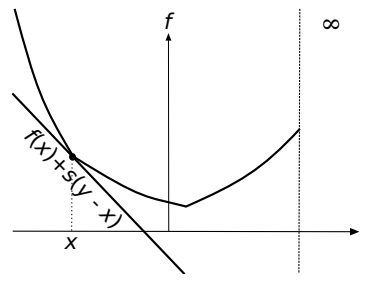
\includegraphics[scale=0.5]{7.png}
\end{center}
For $x$ on the border of dom$(f)$, $\|s\|\rightarrow\infty$, while for $s=0\Rightarrow x$ local/global minimum (but there can be many $s\neq 0$ at local minimum).\\\\
\textbf{Subdifferential} is a set $\partial f(x) =\{s\in \mathbb{R}^n\:|\:s$ is a subgradient at $x\}$
\begin{list}{}{}
	\item $\partial f(x) = \{\nabla f(x)\}\Leftrightarrow f$ differentiable at $x$
	\item $\forall s \in \partial f(x)\:\:\frac{\partial f}{\partial d}(x) \leq \langle s,d\rangle\Rightarrow d$ is a descent direction $\Leftrightarrow \forall s\in\partial f(x)\:\: \langle s,d\rangle < 0$
	\item $s_* = -\arg\min\{\|s\|\:|\:s\in\partial f(x)\}$ \textbf{steepest descent direction}
	\item $x$ \textbf{global minimum} $\Leftrightarrow 0\in \partial f(x)$
\end{list}
\paragraph{Subgradients in $\mathbb{R}^n$} If $\partial f(X) = \{g=\nabla f(x)\}$, $g\perp S(f,f(x))$ i.e. $-g$ points towards $x_*$, then we can take $d\:|\:\langle g,d\rangle < 0$ (descent direction). But if $f$ is nondifferentiable in $x$, there are many different $g$ and all of them are $\perp S(f,f(x))$ ($x$ = kink point), but \textbf{not all of them are descent directions}.\\
However, any (-)subgradient points towards $x_*$:
$$f(x_*)\geq f(x)+\langle g,x_*-x\rangle\Rightarrow \langle g,x_*-x\rangle\leq f(x_*)-f(x)\leq 0$$
Enough for gradient-type approaches.
\paragraph{Convex nondifferentiable optimization is hard} Nondifferentiable optimization is \textbf{orders of magnitude slower}
\begin{center}
	\begin{tabular}{c | c | c | c}
	$f\in C^1$&$\tau$-convex&$L$-smooth&$O\left(\log\left(\frac{1}{\epsilon}\right)\right)$\\
	\hline
	$f\not\in C^1$&$\tau$-convex&$L$-Lipschitz&$\Omega\left(\frac{L^2}{\epsilon}\right)$\\
	\hline
	$f\in C^1$&convex&$L$-smooth&$O\left(\log\left(\frac{1}{\sqrt{\epsilon}}\right)\right)$\\
	\hline
	$f\not\in C^1$&convex&$L$-Lipschitz&$\Omega\left(\frac{L}{\epsilon^2}\right)$
	\end{tabular}
\end{center}
Furthemore, "fixed-step" cannot work for $f\not\in C^1$
\begin{list}{}{}
	\item $f(x) = L|x|,$ $x_0 =-\frac{\alpha L}{2}$
	\item $g_1 = -L,$ $x_1 = x_0 - \alpha g_1 = \frac{\alpha L}{2}$
	\item $g_2 = L,$ $x_2 = x_1 - \alpha g_2 = -\frac{\alpha L}{2} = x_0$
	\item $g_3 = -L\ldots$
\end{list}
$$f_{\text{best}} - f_* = \frac{L^2\alpha}{2}$$
$O(L)$ for $\alpha=\frac{1}{L}$ and the algorithm cycles forever.\\
For $f\in C^1$ \textbf{the gradient is unique}, $d=-\nabla f(x)$:
\begin{list}{}{}
	\item $f(x+\alpha d) < f(x)\:\:\forall\alpha > 0$ small enough
	\item $\|d\|$ is a two-sided proxy of $A(x)$: $\|d\|$ "small" $\Leftrightarrow f(x)$ "close" to $f_*\Leftrightarrow \|d\|\leq \epsilon$ is an effective stopping criterion
	\item Can use fixed step since $\|x_{i+1}-x_i\|\rightarrow 0$ automatically: $\|d_i\|\rightarrow 0$ even if $\alpha_i \geq \tilde{\alpha} > 0$
\end{list}
For $f\not\in C^1$, there can be \textbf{many different subgradients} $d = -[g\in\partial f(x)]$, and for any one of them (can't choose):
\begin{list}{}{}
	\item $f(x+\alpha d)$ may be $\geq f(x)\:\:\forall\alpha$
	\item $\|d\|$ is a \textbf{one}-sided proxy of $A(x)$: $\|d\|$ "small" $\Rightarrow f(x)$ "close" to $f_*$, but $f(x)$ "close" $\not\Rightarrow \|d\|$ "small"! So $\|d\|\leq \epsilon$ is an ineffective stopping criterion (almost never happens)
	\item Can't use fixed step since $\|d\|$ can be big even if $x = x_*$: to ensure $\|x_{i+1}-x_i\|\rightarrow 0$ one has to force $\alpha_i\rightarrow 0$ (but not too fast).
\end{list}
\subsubsection{Subgradient methods}
\paragraph{Fundamental relationship} Any (-)subgradient "points towards $x_*$", so an \textbf{appropriate step} along $-g$ brings closer to $x_*$, meaning that $x_{i+1} = x_i - \alpha_ig_i$ \textbf{makes sense with the right $\alpha_i$}.\\
A fundamental relationship: $$\|x_{i+1}-x_*\|^2 = \|x_i - \alpha_ig_i - x_*\|^2 =$$
$$\|x_i-x_*\|^2+2\alpha_i\langle g_i, x_*-x_i\rangle + \alpha_i^2\|g_i\|^2 \leq \|x_i - x_*\|^2 + \overset{\text{(a)}}{\underset{<0}{\underbrace{2\alpha_i(f_*-f(x_i))}}} + \underset{>0}{\underbrace{\alpha_i^2\|g_i\|^2}} $$
As $\alpha \rightarrow 0$ (short step), the (a) term dominates $\Rightarrow x_{i+1}$ closer to $x_*$ than $x_i$.\\
\textbf{Short but not too short}: \textbf{Diminishing-Square Summable} stepsize (\textbf{DSS}) $$\sum_{i=1}^\infty\alpha_i = \infty\wedge\sum_{i=1}^\infty\alpha_i^2<\infty$$
So $\alpha_i\rightarrow 0$ but not fast enough that the series converges ($\alpha_i = \frac{1}{i}$).\\
DSS just works $$\lim_{i\to\infty} \inf\{f_h\:|\:h\geq i\} = f_*$$
Incredibly robust result: $\alpha_i$ chosen a priori, $f(x_i)$ not even used (only $g_i$), but \textbf{convergence is very slow}.\\
If we knew $f_*$, we could estimate $\alpha_i$, let's assume we do: $$\min\{a\alpha_i^2+2b\alpha_i\}\Leftrightarrow \alpha_i = -\frac{b}{a} = \frac{f(x_i)-f_*}{\|g_i\|^2} \geq 0$$
\textbf{Polyak stepsize} (\textbf{PSS}): $$\alpha_i = \beta_i\frac{f(x_i)-f_*}{\|g_i\|^2}$$ With $\beta_i = 1$ we have a "optimal step", but works $\forall\:\beta_i\in(0,2)$ since this $\Rightarrow \|x_{i+1}-x_*\|^2 < \|x_i-x_*\|^2\Rightarrow \{x_i\}\rightarrow x_*$\\
In pratice is vastly better, but as far as it can go (not much): $\min\{f(x_h)\:|\:g\leq i\}-f_*\leq L\frac{\|x_1-x_*\|}{\sqrt{i}}\Rightarrow O\left(\frac{1}{\epsilon^2}\right)$\\
From $\epsilon=1$e$-3$ to $\epsilon=1$e$-4$ we get 100x the iterations. The good news is that PSS would be optimal if we knew $f_*$, which we don't $\rightarrow$ \textbf{target level stepsize} (vanishing), "\textit{if you don't know it estimate it, but be ready to revise your estimate}".\\
Reference value $f_{ref} -$ threshold $\delta =$ target level $\simeq f_*$. With a "good improvement", $f_{ref}$ gets smaller and also does the target level. If there are too many steps without improvement, $\delta$ gets smaller so the target level increases.\\
\textbf{Too many parameters}: $\rho\in(0,1),\beta\in(0,2),\delta_0>0,R>0$\\
$\{f_{rec,i}\}\rightarrow f_*$ but there's no reasonable stopping criterion, just "stop after a while". So slow convergence.
\paragraph{Deflected Subgradient} Better model, better direction. There's no second-order information but deflection is possible $$d_i = \gamma_ig_i+(1-\gamma_i)d_{i-1}$$ $$\:x_{i+1}=x_i-\alpha_id_i\simeq \text{"Conjugate Subgradient"}$$
To have theoretical convergence, there are some rules:
\begin{multicols}{2}
\begin{center}
	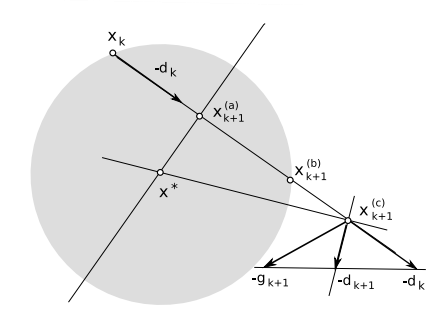
\includegraphics[scale=0.66]{8.png}
\end{center}
\columnbreak
\begin{list}{}{}
	\item \textbf{Stepsize-restricted}, deflection-first\\
	$$\alpha_i = \beta_i\frac{f(x_i)-f_*}{\|d_i\|^2}\wedge\beta_i\leq\gamma_i$$
	"As deflection increases, stepsize has to decrease".
	\item \textbf{Deflection-restricted}, stepsize-first\\
	$$\frac{\alpha_{i-1}\|d_{i-1}\|^2}{(f(x_i)-f_*)+\alpha_{i-1}\|d_{i-1}\|^2}\leq \gamma_i$$
	"As $f(x_i)$ approaches $f_*$, deflection has to decrease"
\end{list}
\end{multicols}
In both cases, target level to replace $f_*$.\\
A closed formula: $\gamma_i\in$ $\arg\min\{\|\gamma g_i+(1-\gamma)d_{i-1}\|^2\:|\:\gamma\in[0,1]\}$
\subsubsection{Smoothed Gradient Methods} The speed is a property of the space, so let's change the space. Requires $f(x) = \max\{x^TAz\:|\:z\in Z\}$ convex and assumed to be easy to compute. $\tilde{z}$ optimal for $x\Rightarrow A\tilde{z}\in\partial f(x)\Rightarrow f\not\in C^1$ (there can be many different $\tilde{z}$).\\
\textbf{Smoothed} $$f_\mu(x)=\max\left\{x^TAz-\mu\frac{\|z\|^2}{2}\:|\:z\in Z\right\}\in C^1$$ Hopefully easy. Choose small $\mu=O(\epsilon)$, with fast minimization of $f_\mu$ gives only $O(\frac{1}{\epsilon})$.\\
In practice is slowish, superlinear in a doubly-logarithmic chart after a long flat leg. Subgradients are faster but flatline at $\epsilon\simeq 1$e$-4$, smoothed does at $\epsilon\simeq 1$e$-6$.
\subsubsection{Bundle Methods}
\paragraph{Basic Idea} Cutting-plane model. Being $f$ convex, the first-order information that we have is globally valid: I can collect it along the way and use it all.\\
$\{x_i\}\rightarrow$ bundle $$\mathscr{B}=\{(x_i, f_i = f(x_i), g_i\in\partial f(x_i))\} = \{(x_i, f_i, g_i)\}$$
The \textbf{cutting-plane model} $f_\mathscr{B}$ of $f$ is $$f_\mathscr{B}(x) = \max\{f_i+\langle g_i, x-x_i\rangle\:|\:(x_i, f_i, g_i)\in \mathscr{B}\}\leq f(x)\:\:\forall x$$ A $(1+\epsilon)$-order model.
$$x_{\mathscr{B},*}\in \arg\min\{f_\mathscr{B}(x)\}$$ $$f_\mathscr{B}(x_{\mathscr{B},*})\leq f_*$$ Use $x_{\mathscr{B},*}$ as the next iterate a-la Newton.\\
$f_\mathscr{B}\not\in C^1$ but computing $x_{\mathscr{B},*}$ is a linear program $\Rightarrow$ easy if $\# \mathscr{B}$ "small" $$\min\{f_\mathscr{B}(x)\}=\min\{v\:|\:v\geq f_i+\langle g_i, x-x_i\rangle\:\:(x_i, f_i, g_i)\in \mathscr{B}\}$$
\paragraph{Cutting Plane Algorithm} $\min\{f_\mathscr{B}(x)\}$ is the master problem, and $(x_*, v_*)$ the optimal solutions $\rightarrow$ new $(x_*, f(x_*), g_*\in\partial f(x_*))$\\
$f(x_*)\leq v_*\Rightarrow x_*$ optimal, otherwise $\mathscr{B}= \mathscr{B}\:\cup\:(x_*, f(x_*), g_*)\Rightarrow f_\mathscr{B}$ becomes a better model.\\
The min in the master problem focuses $\{x_*\}$ in the right place, with a practical stopping criterion (unlike any subgradient-style algorithm). But $\#\mathscr{B}\rightarrow\infty\Rightarrow$ the cost per iteration of the master problem $\rightarrow\infty$.\\
So the practical convergence is often horrible, can be $O\left( \left(\frac{1}{\epsilon}\right)^{\frac{n}{2}}\right)$
\subparagraph{Why} $x_{\mathscr{B},*}$ \textbf{may be infinitely far} from $x_*$, the \textbf{iterates have no local property} ($\|x_{i+1}-x_i\|$ can be very large and doesn't go smoothly to $0$, no fast convergence in the tail).\\
It's unavoidable: linear functions have no curvature, and we need many linear functions to make a quadratic one. Pruning $\mathscr{B}$ is possible but not easy, and no a priori bound on $\# \mathscr{B}$.
\subparagraph{Stabilizing} $\overline{x}$ as stability center (the best $x_i$ so far) with $\mu$ stability parameter (how far from $\overline{x} f_\mathscr{B}$ is a good model of $f$).\\
Stabilized master problem $$\min\left\{f_\mathscr{B}(x)+\mu\frac{\|x-\overline{x}\|^2}{2}\right\}$$ Keeps $\{x_*\}$ "close" to $\overline{x}$ (perhaps too close if $\mu$ too large). When $\mu$ too small, unstabilized cutting plane.
\section{Constrained Optimality and Duality}
\paragraph{Constrained Optimization} Back to the full $$(P)\:\:\:\:\:f_* = \min\{f(x)\:|\:x\in X\}$$ with $x\subset R^n$\begin{list}{}{}
	\item $x\in X$ are \textbf{constraints}, hence constrained optimization
	\item $x\in X$ feasible solution, $x\not\in X$ unfeasible solution
	\item $x_*\in X\:|\:f(x_*)\leq f(x)\:\:\forall\:x\in X$ optimal solution $\Leftrightarrow$ global optimum
\end{list}
Constraints can be hidden in the objective $\chi_X : \mathbb{R}^n\rightarrow \overline{\mathbb{R}}$ \textbf{indicator function of $X$} with $$\chi_X(x)=\left\{\begin{array}{l l}
0&\text{if }x\in X\\
\infty&\text{if }x\not\in X
\end{array}\right.$$ Convex if $X$ is, but extended-valued.
$$(P)\Leftrightarrow \min\{f_X(x)=f(x)+\chi_X(x)\}$$ Which is essential the objective, a very bad idea: $\chi_X\not\in C^1$! Conversely, objective "complex" $\rightarrow$ "simple" by "hiding it in the constraints".
$$(P)\Leftrightarrow\min\{v\:|\:v\geq f(x), x\in X\}$$
\paragraph{(Local) minima vs. optima} Note that $X=\emptyset\Rightarrow v(P) = +\infty$, so solving $(P)$ includes constructively proving $X=\emptyset$. Almost never happens in ML, so we will forget about this but the issue exists. The model is our choice, we choose it simple/nice/nonempty if we can.\\
Global optimum obviously hard, hence $x_*$ local optimum solves $$\min\{f(x)\:|\:x\in B(x_*,\epsilon)\cap X\}$$ for some $\epsilon>0$.\\
Important concept: $x$ in the interior of $X\Leftrightarrow\exists\:B(x,\epsilon)\subseteq X$ (for $\epsilon>0$), so $x_*$ in the interior of $X\Rightarrow$ local minimum/optimum so $\nabla f(x_*)=0$.\\
Constrained (local) optimality conditions $\neq\nabla f(x)=0$, only if $x$ not in the interior $\Leftrightarrow x\in \partial X$, the boundary of $X$.
\subsection{First-Order Optimality Conditions}
\subsubsection{Geometric Version}
\paragraph{The Tangent Cone} Crucial Object $T_X(x) =$ tangent cone of $X$ at $x$
$$T_X(x) = \left\{d\in \mathbb{R}^n\:|\:\exists\{z_i\in X\}\rightarrow x\wedge \{t_i\geq 0\}\rightarrow 0, d=\lim_{i\to\infty}\frac{z_i-x}{t_i}\right\}$$
Tangent Cone Condition (TCC): $\langle\nabla f(x),d\rangle \geq 0\:\:\forall d\in T_X(x)$\\Zooming into $x$, $X$ looks like a cone, so we build the cone $T_X(x)$ with $x$ as the vertex.
\begin{center}
	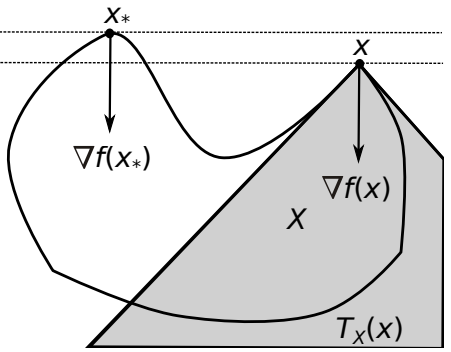
\includegraphics[scale=0.75]{9.png}
\end{center}
Note that TCC $\not\Rightarrow$ local optimum, even less global optimum, \textbf{unless} $X$ is such that $X\subseteq x + T_X(x)$\\
Turns out that $X$ convex $\Rightarrow$ this.
\paragraph{Convex Sets} $x,y\in \mathbb{R}^n,\{z=\alpha x+(1-\alpha)y\:|\:\alpha\in[0,1]\} = \text{conv}(x,y) =$ segment joining $x$ and $y$
\begin{list}{}{}
	\item $C\subset \mathbb{R}^n$ \textbf{convex}: $\forall\:x,y\in C\:\:\text{conv}(x,y)\subseteq C$
	\item $C\subset \mathbb{R}^n$ \textbf{nonconvex}: $\exists\:x,y\in C\:|\:\text{conv}(x,y)\not\subseteq C$
\end{list}
Being convex is rare: nonconnected $\Rightarrow$ nonconvex. Every nonconvex set can be "completed" to a convex set (\textbf{convex hull}):
$$\text{conv}(S) = \bigcup\{\text{conv}(x,y)\:|\:x,y\in S\} = \bigcap\{C\:|\:C\text{ is convex}\wedge C\supseteq S\}$$
Meaning, respectively, "iterated convex hull of all $x,y\in S$" = "smallest convex set containing $S$".\begin{list}{}{}
	\item $C$ convex $\Leftrightarrow C = \text{conv}(C)$: a convex set is equal to its convex hull
	\item $f$ convex $\Leftrightarrow epi(f)$ convex $\Rightarrow S(f,v)$ convex $\forall v$ ($\not\Leftarrow$)
	\item $d$ is a \textbf{feasible direction} of $X$ at $x$ if $\exists\:\tilde{\epsilon}>0\:|\:x+\tilde{\epsilon}d \in X$
	\item $F_X(x)$ is the \textbf{set of feasible directions of $X$ at $x$}
	\item $X$ convex and $d\in F_X(x)\Rightarrow x+\epsilon d\in X\:\:\forall
	\epsilon\in [0,\tilde{\epsilon}]$ ($F_X$ cone)
	\item $X$ convex and $d$ feasible at $x \Rightarrow d\in T_X(x)$ with $z_i = x + dt_i \Leftrightarrow F_X(x)\subseteq T_X(x)$\\
	In fact they are almost the same, except from the borders
	\item $f,X$ convex, $x_*$ global optimum $\Leftrightarrow\langle\nabla f(x_*),d\rangle \geq 0\:\:\forall\:d\in F_X(x_*)$
	\item $f,X$ convex, (TCC) at $x_*\Rightarrow x_*$ global optimum
	\item $x_*$ global optimum $\Rightarrow x_*$ local optimum $\Rightarrow$ (TCC)
\end{list}
(TCC) sufficient in the convex case, but is always necessary. Not always sufficient because it holds in saddle point of $\partial X$, for example, despite not being a minimum.\\
$\nabla f(x) = 0\Rightarrow \langle\nabla f(x),d\rangle = 0\:\:\forall\:d\in \mathbb{R}^n \Rightarrow$ (TCC), so a feasible local minimum is a local optimum regardless of $X$. Conversely, $x\in$ int$(X)\Rightarrow T_X(x) = F_X(x) = \mathbb{R}^n$ hence (TCC) $\Leftrightarrow\langle\nabla f(x),d\rangle \geq 0\:\:\forall\:d\in \mathbb{R}^n\Leftrightarrow \nabla f(x) = 0$\\
In fact, $f,X$ convex $\Rightarrow$ (TCC) $\Leftrightarrow \not\exists$ feasible descent direction: every direction is feasible, hence only descent matters. So "$x$ satifies (TCC)" is a direct constrained generalization of "$x$ stationary point".\\
Necessary, \textbf{not sufficient} but the only one you can reasonably check. But how to compute this in practice? How to prove something doesn't exists? How to characterize $T_X$ depends on how you characterize $X$.
\subsubsection{Algebraic Version}
\paragraph{Describing a Set via Functions} The most used way to describe a set is via some functions.\\
The obvious ways is via constraints:
\begin{list}{}{}
	\item \textbf{Inequality constraints} $f(x)\leq\delta$, \textbf{sublevel set $S(f,\delta)$}
	\item \textbf{Equality constraints} $f(x)=\delta$, \textbf{level set $L(f,\delta)$}
	\item For convenience, $\delta$ can be hidden in $f$ so $f(x)\leq0,f(x)=0$
	\item If one wants $f(x)\geq 0$ simply $-f(x)\leq 0$
\end{list}
Usually multiple constraints, $f_1(x)\leq 0, f_2(x)\leq 0$ means logical conjunction (first condition \textit{and} second condition), so an \textbf{intersection} of (sub) level sets.\\\\
One of the standard forms of constrained nonlinear optimization:
$$X=\{x\in \mathbb{R}^n\:|\:g_i(x)\leq 0\:\:i\in I, h_j(x)=0\:\:j\in J\}$$
with $I$ set of inequality constraints and $J$ set of equality constraints. Often useful is the compact version via vector-valued functions:
\begin{list}{}{}
	\item $G(x) = [g_i(x)]_{i\in I} : R^n\rightarrow R^{|I|}$
	\item $H(x) = [h_j(x)]_{j\in J} : R^n\rightarrow R^{|J|}$
	\item $X=\{x\in \mathbb{R}^n\:|\:G(x)\leq 0, H(x) = 0\}$
\end{list}
There are \textbf{many different ways to express the same $X$}, a concept called \textbf{reformulation}. Often, choosing the right formulation is crucial for being able to solve a problem. We will not see this, but a few trivial observation are useful:
\begin{list}{}{}
	\item Could always assume $|J|=0$, no equality constraints: $h_j(x) = 0\Leftrightarrow h_j(x)\leq 0, -h_j(x)\leq 0$\\
	One equality constraints $\Leftrightarrow$ two "opposite" inequality constraints
	\item Could always assume $|I|=1$, one single inequality constraint\\
	$G(x)\leq 0\Leftrightarrow \max\{g_i(x)\:|\:i\in I\} = g(x)\leq 0$
\end{list}
This can be useful to simplify the notation, but almost never useful for implementation: \textbf{exploit the structure of $X$ and of the constraints when is there}.\\
Also, reformulations can be bad: $\max\{g_1,g_2\}\not\in C^1$ even if both $g_1\in C^1$ and $g_2\in C^1$.
\paragraph{Convex Sets out of Convex Functions} How can I be sure of the convexity of $X$?\\
Sublevel sets of convex functions are convex $\Rightarrow g_i(x)\leq 0$ with $g_i$ convex "good"\begin{list}{}{}
	\item $g_i(x) \geq 0$ not convex if $g_i$ is, and typically is badly not convex (reverse convex)
	\item $g_i(x) \geq 0$ convex if $g_i$ concave, but $g_i(x) \leq 0$ is not
	\item $g_i(x) = 0$ convex only if $g_i(x)\leq 0$ convex and $g_i(x) \geq 0$ convex, so $g_i$ is both convex and concave, meaning $g_i$ is linear
\end{list}
So, \textbf{to have a convex $X$ all equality constraints must be linear}.
\paragraph{Linear Equality Constraints} $$(P)\:\:\:\:\:\min\{f(x)\:|\:Ax=b\}$$
With $g_i(x) = \langle A_i, x\rangle$ linear (affine), $\nabla g_i(x) = A_i \perp S(g_i,\:)$
\begin{list}{}{}
	\item \textbf{Half space} $\langle A_i, x\rangle + b_i\leq 0$\\
	It's full dimensional, thus it has an "interior".
	\item \textbf{Hyperplane} $\langle A_i, x\rangle + b_i\equiv 0$, which is the same as $\langle A_i, x\rangle + b_i\leq 0\land \langle -A_i, x\rangle + b_i\leq 0$\\
	It's not full dimensional, due to having $n-1$ dimensions, thus it has no interior.
\end{list}
$k$ constraints form a subspace, a polyhedral cone in the case of inequality constraints, unless they are linearly dependant or with same solutions.\\
In a simple case, $(P)$ defined by $\min\{f(x)\:|\:Ax=b\}$
\begin{list}{}{}
	\item $x\in X \Leftrightarrow x\in \partial X$ plus "$\partial X$ looks the same everywhere".
	\item $S(f,\cdot)$ and $X=\{x\in \mathbb{R}^n\:|\:Ax=b\}$: optimum touches the inner level set.
	\item $F_X(x) = \{d\in \mathbb{R}^n\:|\:Ad=0\}\:\:\forall\:x$: for any $y\in X$ necessarily $y-x = d\perp A$
	\item (TCC) $\Leftrightarrow \langle\nabla f(x),d\rangle = 0\:\:\forall\:d\in F$ as $d\in F\Rightarrow -d\in F$
	\item $d\perp A$ and $\nabla f(x)\perp d$ means $\nabla f(x)$ parallel to $A\Leftrightarrow\nabla f(x)\in $ range$(A)\Leftrightarrow\exists\:\mu\in \mathbb{R}^m\:|\:\nabla f(x) = \mu A$
	\item Poorman's KKT conditions: $Ax = b \wedge \exists\:\mu\in \mathbb{R}^m\:|\:\mu A = \nabla f(x)$
	\item $f$ convex $\Rightarrow$ (P-KKT) sufficient for global optimality.
\end{list}
\paragraph{Nonlinear Inequalities} $T_X(x) = T_{X\cap B(x,\epsilon)}(x)$: only what happens as $x_i\rightarrow x$ matters $\Rightarrow$ if $x\not\in \partial S(g_i,0)$ then constraint $g_i(\cdot)\leq 0$ has no impact on $T_X(x)$\\
$x\in\partial s(g_i,0)\Rightarrow g_i(x)=0$ (but $\not\Leftarrow$)\\
Active constraints at $x\in X$: $\mathscr{A}(x) = \{i\in I\:|\:g_i(x)=0\}\subseteq I$\\
\textbf{First-order feasible direction cone} at $x\in X$: $$D_X(x) = \{d\in \mathbb{R}^n\:|\:\langle\nabla g_i(x), d\rangle\leq 0\:\:i\in A(x),\langle\nabla h_j(x),d\rangle = 0\:\:j\in J\}=$$ $$=\{d\in \mathbb{R}^n\:|\:(JG_{A(x)}(x))d\leq 0, (JH(x))d=0\}$$
\paragraph{Farkas' Lemma} $D_X$ is a polyhedral cone: $C=\{d\in \mathbb{R}^n\:|\:Ad\leq 0\}$ for some $A\in \mathbb{R}^{k\times n}$, very close to $\partial X$ looks like a polyhedron.\\
Dual cone $C^*=\{c=\sum_{i=1}^k\lambda_iA_i\:|\:\lambda \geq 0\}$\\
\textbf{Farkas' Lemma}: $\forall\:c\in \mathbb{R}^n$:
\begin{list}{}{}
	\item either $\exists\:\lambda\geq 0\:|\:c = \sum_{i=1}^k \lambda_iA_i$
	\item or $\exists\:d\:|\:Ad\leq 0\wedge\langle c,d\rangle > 0$
\end{list}
One and only one is true.\\
$\langle c,d\rangle \leq 0\:\:\forall\:d\in C, c\in C^*$ actually a $\neq$ definition: polar cone $C^\circ=\{c\in \mathbb{R}^n\:|\:\langle c,d\rangle\leq 0\:\:\forall\:d\in C\}=C^*$ so Farkas' lemma says that $\forall\:c\in \mathbb{R}^n$ either $c\in C^*$ or $c\not\in C^*$\\\\
$x_*$ optimum $\Rightarrow \langle\nabla f(x_*),d\rangle\geq 0\:\:\forall\:d\:|\:$
\begin{list}{}{}
	\item $\langle\nabla g_i(x_*),d\rangle\leq 0\:\:i\in A(x)$
	\item $\langle\nabla h_j(x_*),d\rangle = 0\:\:j\in J$
\end{list}
$\Leftrightarrow\lambda\in \mathbb{R}_+^{|A(x)|}$ and $\mu \in \mathbb{R}^{|J|}\:|\:\nabla f(x_*) + \sum_{i\in A(x)}\lambda_i\nabla g_i(x_*) + \sum_{j\in J} \mu_j\nabla h_j(x_*)=0$\\
So a constructive way to prove the conditions is to find $\lambda$ and $\mu$.
\paragraph{KKT Conditions} $\exists\:\lambda\in \mathbb{R}_+^{|I|}$ and $\mu\in \mathbb{R}^{|J|}\:|$\begin{list}{}{}
	\item[(KKT-F)] $g_i(x)\leq 0\:\:i\in I$, $h_j(x) = 0\:\:j\in J$
	\item[(KKT-G)] $\nabla f(x) + \sum_{i\in I}\lambda_i\nabla g_i(x) + \sum_{j\in J}\mu_h\nabla h_j(x) = 0$
	\item[(KKT-CS)] $\sum_{i\in I}\lambda_i(-g_i(x)) = 0$ \textbf{complementary slackness} $\Leftrightarrow \lambda_ig_i(x) = 0\:\:\forall\:i\in I$
\end{list}
\paragraph{KKT Theorem} $T_X(x)=D_X(x)\wedge x$ local optimum $\Rightarrow$ (KKT)\\
For $(P)$ convex, (KKT) $\Rightarrow x$ global optimum: (KKT) $\Rightarrow \langle \nabla f(x), d\rangle \geq 0\:\:\forall\:d\in D_X(x)$ and $D_X(x)\supseteq T_X(x)\supseteq F_X(x) \Rightarrow\langle \nabla f(x), d\rangle \geq 0\:\:\forall\:d\in F_X(x)\Rightarrow x$ global optimum.
\subsection{Second-Order Optimization}
If $(P)$ is not convex then (KKT) is not sufficient, need to use second order but clearly not just "$\nabla^2 f(x_*)\succeq 0$". Fundamental concept: \textbf{Lagrangian function} $$L(x;\lambda, \mu)=f(x) + \sum_{i\in I} \lambda_ig_i(x) + \sum_{j\in J}\mu_jh_j(x)$$ with $x$ variables and $\lambda,\mu$ parameters. Fundamental observation $(x,\lambda,\mu)$ satisfies (KKT-G) $\Leftrightarrow \nabla L(x;\lambda,\mu) = 0$ (gradient on $x$ alone) $\Rightarrow x$ stationary point of $L(\cdot;\lambda,\mu)$. When a stationary point is also a minimum?
\paragraph{Lagrangian Relaxation} Lagrangian function is objective and constraints together. (KKT-G) $\Leftrightarrow x$ stationary point of $L()$ for the right $\lambda\geq 0$ and $\mu$. Assume we know them, can we find $x$?\\
Natural idea: solve the Lagrangian relaxation $$(R_{\lambda,\mu})\:\:\psi(\lambda,\mu) = \min_x\{L(x;\lambda, \mu)\:|\:x\in \mathbb{R}^n\}$$
The relaxation is another optimization problem carefully constructed in order to provide a lower bound on $v(P)$ for $(P)\:\:\min\{f(x)\:|\:x\in X\}$\\
$(\underline{P})\:\:\min\{\underline{f}(x)\:|\:x\in \underline{X}\}$ relaxation of $(P) \Rightarrow v(\underline{P})\leq v(P)$ if $\underline{X}\supseteq X$ and $\underline{f}(x)\leq f(x)\:\:\forall\:x\in X$\\
$(R_{\lambda,\mu})$ is a relaxation of $(P)\:\:\forall\:\lambda\geq 0$ and $\mu\Rightarrow$ weak duality $\forall\:\:x\in X$, $\psi(\lambda,\mu)\leq v(P)\leq f(x)$\\
But how to choose $\lambda\geq 0$ and $\mu$? The dual function $\psi$ is \begin{list}{}{}
	\item Often easy to compute
	\item Concave, but note that $\psi(\lambda,\mu)=-\infty$ might happen
	\item $\tilde{x}$ optimal in ($R_{\lambda,\mu}$) $\Rightarrow [G(\tilde{x}), H(\tilde{x})]\in \partial\psi(\lambda,\mu)$
	\item $\psi\not\in C^1$ even if $f,g_i,h_j$ are, but $\tilde{x}$ unique optimal solution to ($R_{\lambda,\mu}$) $\Rightarrow \psi$ differentiable in $(\lambda, \mu)$, $\nabla \psi(\lambda, \mu)= [G(\tilde{x}), H(\tilde{x})]$
\end{list}
The first three properties makes $\psi$ easy to maximize, so a Langragian dual of $(P)$ $$(D)\:\:\max\{\psi(\lambda,\mu)\:|\:\lambda\in \mathbb{R}_+^{|I|},\mu\in \mathbb{R}^{|J|}\}$$ But it needs to be solved to global optimality and not necessarily convex, but if you can do that everything works even on $(P)$ nonconvex.\\
When is $v(D) = v(P)$ (strong duality)?  \textbf{Convexity} $\Rightarrow$ \textbf{Strong Duality}, so not always but yes if $(P)$ convex, meaning that $x_*$ optimum, $T_X(x_*)=D_X(x_*)\Rightarrow v(D) = v(P)$\\
Under further conditions, solving $(D)$ actually solves $(P)$
\paragraph{Specialized Lagrangians} Lagrangian dual is powerful but cumbersome: $\min$/$\max$, simplifies to have "just max".\begin{list}{}{}
	\item For linear programs $(P)\:\:\min\{cx\:|\:Ax\geq b\}$\\
	$L(x;\lambda) = cs + \lambda(b-Ax)=\lambda +(c-\lambda A)x$ lagrangian function\\
	$\psi(\lambda)=\min_{x\in \mathbb{R}^n} L(x;\lambda)=\left\{\begin{array}{l l}
	-\infty& \text{if }c-\lambda A\neq 0\\
	0& \text{if }c-\lambda A= 0\\
	\end{array}\right.$\\
	$(D)\:\:\max\{\psi(\lambda)\:|\:\lambda\geq 0\}=\max\{\lambda b\:|\:\lambda A=c, \lambda\geq 0\}$ a different linear program with the same data.\\
	Strong duality almost always holds.
	\item For quadratic programs $(P)\:\:\min\{\frac{1}{2}\|x\|_2^2\:|\:Ax = b\}$\\
	 $L(x;\mu)=\frac{1}{2}\|x\|_2^2+\mu(Ax-b)$\\
	 $\psi(\mu)=\min_{x\in \mathbb{R}^n} L(x;\mu)$ hence $\nabla L(x)=x+\mu A = 0 \Leftrightarrow x = - \mu A\Rightarrow \psi(\mu)=-\frac{1}{2}\mu^T(AA^T)\mu - \mu b$\\
	 $(D)\:\:\max\{-\frac{1}{2}\mu^T(AA^T)\mu-\mu b\:|\:\mu \in \mathbb{R}^m\}$ (an unconstrained quadratic program). It's strictly convex and strong duality almost always holds with $(D)\:\:\max\{\lambda b-\frac{1}{2}v^TQ^{-1}v\:|\:\lambda A-v=q, \lambda\geq 0\}$
\end{list}
\subsection{Constrained Optimization Algorithms} Algorithms for $$(P)\:\:\min\{f(x)\:|\:G(x)\leq 0, H(x) = 0\}$$
Usually it's ok to ignore $H(x)$, just $G(x)\leq 0$ (implementation details). Only linear inequalities $Ax\leq b$, because of their convenience: always convex, satisfy (Linl), numerically stable, cheap to compute\ldots\\
Important notation of \textbf{sub-system} (a relaxation): given $A\in \mathbb{R}^{m\times n}, b\in \mathbb{R}^m$ we define $B\subseteq\{1,2,\ldots,m\}$ subset of row's indexes (constraints) $\Rightarrow$ sub-matrix/vector/system $$A_B=[A_i]_{i\in B}$$ $$b_B=[b_i]_{i\in B}$$ $$A_Bx \leq b_B$$
\textbf{Polyhedral cone} $$F_X(x)=\{d\in \mathbb{R}^n\:|\:A_{\mathscr{A}(x)} d\leq 0\}$$ with $\mathscr{A}(x)$ being the 
\textbf{active constraints} at $x\in X$: $$\mathscr{A}(x) = \{i\in I\:|\:g_i(x)=0\}\subseteq I$$
\subsubsection{Quadratic Problem with Linear Equality Constraints}
\paragraph{Equality-Constrained QP} $$(P)\:\:\min\left\{\frac{1}{2}x^TQx+qx\:|\:Ax=b\right\}$$ with $A\in \mathbb{R}^{m\times n}$, $\text{rank}(A)=m<n \Leftrightarrow$ rows of $A$ are linearly independent. Usually $(P)$ convex $\Leftrightarrow Q\succeq 0$ (otherwise $v(P)=-\infty$ likely).\\
For a minimum/saddle point, just solve the $KKT$ system (normal equations)
$$\begin{array}{c}
(a)\\(b)
\end{array}\left[\begin{array}{c c}
Q&A^T\\A&0
\end{array}\right]\left[\begin{array}{c}
x\\\mu
\end{array}\right]=\left[\begin{array}{c}
-q\\b
\end{array}\right]$$\\
Just linear algebra, symmetric but indefinite, lots of 0 eigenvalues. It's a basic step in many cases, so need to do that efficiently: just go and solve it by direct or iterative methods
\begin{list}{}{}
	\item indefinite factorization of the matrix (may reduce sparsity)
	\item Krylov-type iterative methods (GMRES,\ldots)
\end{list}
or try to exploit the large scale structure (saddle-point system).
\paragraph{Active-Set Method} Quadratic program with linear constraints. If one knew $\mathscr{A}(x_*)$, then it would be "just linear algebra" $\Rightarrow$ \textit{if you don't know it estimate it but be ready to revise your estimate}: we estimate the active set with $B$, current estimate of $\mathscr{A}(x_*)$.
\begin{center}
	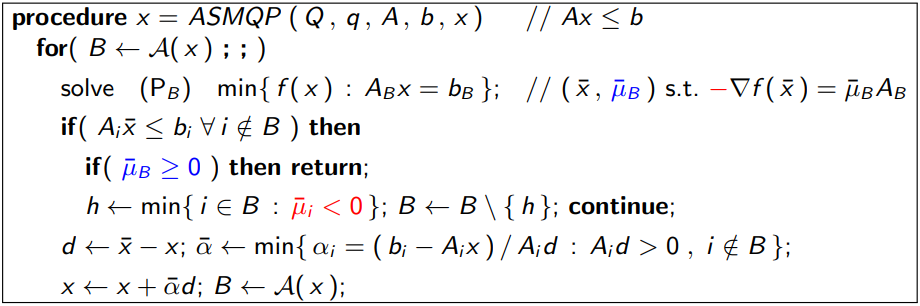
\includegraphics[scale=0.75]{10.png}
\end{center}
Can compute feasible initial $x$ autonomously.\\
\textbf{Always exploit all the structure of your problem}: quadratic program with \textbf{box constraints} $$(P)\:\:\min\left\{\frac{1}{2}x^TQx+qx\:|\:\underline{x}\leq x\leq \overline{x}\right\}$$
Active constraint $\Leftrightarrow$ inactive variable: $B\subseteq \mathbb{N}=\{1,2,\ldots,n\}$ \\$B = (L,U)$ with
\begin{list}{}{}
	\item $L\cap U=\emptyset$
	\item $L\cup U \subset \mathbb{N}$
	\item $F = N\setminus (L\cup U)$
\end{list}
$\Rightarrow A_Bx=b_B \Leftrightarrow x = [x_L, x_F, x_U]=[\underline{x}_L, x_F, \tilde{x}_U]$ So only $x_F$ "free".\\
$\underline{x} = 0 (x\leftarrow x+\underline{x})\Rightarrow x=[0, x_F, \tilde{x}_U]$\\
$(P)$ can become $$(P)\:\:\min\left\{\frac{1}{2}x_F^TQ_{FF}x_F+(q_F+\overline{x}_U^TQ_{UF})x_F\right\}$$ \textbf{unconstrained} and in a (possibly much) smaller space. Initial feasible $x$ straightforward.
\subparagraph{In practice} If (Linl)-type not satisfied, $B$ needs to be more carefully managed to handle possible degenerate steps $(\tilde{\alpha}=0)$. For instance, only one constraint at a time is added to $B$, not very efficient in practice and different nontrivial rules are used.\\
Exploit information from previous iteration to speed up KKT system solution: update factorizations, use $x$ to warm-start iterative approaches\ldots many different variants.\\
No more exact solution but hopefully fast iterative approaches, e.g. (quasi-)Newton on the reduced problem.\\
Which $\epsilon$? How many iterations? How about one of the gradient methods?
\subsubsection{Projected Gradient Method} Nonlinear problem with linear constraints $(P)\:\:\min\{f(x)\:|\:Ax\leq b\}$, feasible $x$: if $-\nabla f(x)\in F_X(x)$ trivial, just LS/FS along $d=-\nabla f(x)$. In general, find $d\in F_X(x)$ "closer" to $-\nabla f(x)$ then FS/LS along $d$.\\
Projection of $d\in \mathbb{R}^n$ on $S\subset R^n$: $$p_S(d)=\min\left\{\|d-x\|\:|\:x\in S\right\}$$ $$p_{F_X(x)}(-\nabla f(x))=\min\left\{\frac{\|d+\nabla f(x)\|^2}{2}\:|\:A_{\mathscr{A}(x)}d\leq 0\right\}$$
a convex quadratic program with simple function on a polyhedral cone. Non trivial but clearly doable, for example ASMQP. $d_*=0\Rightarrow \lambda_*A_{\mathscr{A}(x)}+\nabla f(x) = 0, \lambda_* \geq 0\Leftrightarrow x$ optimal for $(P)\Rightarrow$ stopping condition $\|d_*\|\leq \epsilon$ (norm of projected gradient).\\
$p_{F_X(x)}(\:)$ potentially costly but can be very cheap with appropriate $X$.
\paragraph{Special Forms of Constraints} Always exploit all the structure of your problem: box constraints $\underline{x}\leq x\leq \tilde{x}$: $X$ decomposable $= X_1\times \ldots \times X_n$ with $X_i=[\underline{x}_i, \tilde{x}_i] \Rightarrow$ $$F_X(x) = \bigotimes_{i=1}^n F_{X_i}(x_i)$$ $$F_{[\underline{x},\tilde{x}]}(x) = \left\{\begin{array}{cl}
\mathbb{R}_+&\text{ if }x=\underline{x}\\
\mathbb{R}_-&\text{ if }x=\overline{x}\\
\mathbb{R}&\text{ otherwise}\\
\end{array} \right.$$
$g(d) = \|d-v\|^2$ decomposable: $$g(d)=\sum_{i=1}^n [g_i(d_i)=(d_i-v_i)^2]$$
$p_X(x)$ separable $\Rightarrow n$ independent problems, much easier and parallelizable.
\begin{center}
	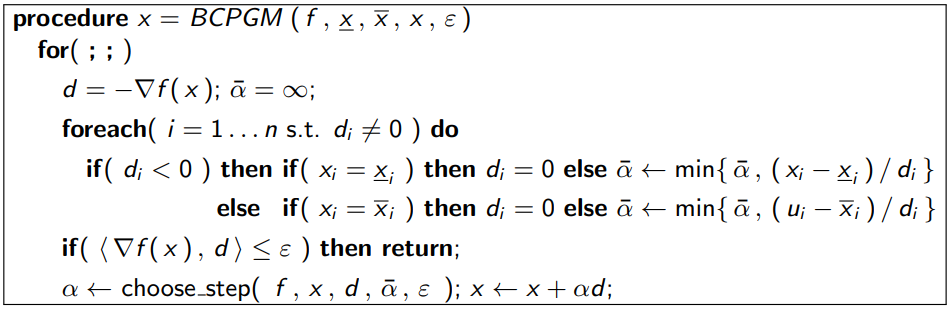
\includegraphics[scale=0.75]{11.png}
\end{center}
Other cases where projection is easy: simplex constraints $\sum_{i=1}^n x_i = 1, x_i\geq 0$ for $i=1,\ldots,n$.
\paragraph{Goldstein's Version} What if projection is easy on the whole $X$, not only $F_X(x)$? Goldstein's projected gradient method: move first, project second $$y_i = x_i - \alpha_i\nabla f(x_i)$$ $$x_{i+1}= p_X(y_i)$$
Not a descent method, more like a heavy ball, and only converges with appropriate stepsize, typical $\alpha=\frac{1}{L}$. Convergence result similar to unconstrained gradient (for good and bad): $O\left(\left(\frac{L}{\tau}\right)\log\left(\frac{1}{\epsilon}\right)\right)$ for $f$ $\tau$-convex, $O\left(\frac{LD}{\epsilon}\right)$ otherwise.
\paragraph{Rosen's Version} General $Ax\leq b$: $p_{F_X(x)}$ can be too costly.\\
Make it easier by projecting on $$\partial F_X(x)=\{d\in \mathbb{R}^n\:|\:A_{\mathscr{A}}d=0\}$$ Quadratic program with easy objective and equality constraints, so very easy. In fact, $\overline{A}=A_{\mathscr{A}(x)}$ full row rank $\Rightarrow$ closed formula
$$\mu=-[\overline{A}\,\overline{A}^T]^{-1}\overline{A}\nabla f(x)$$
$$d = (I-\overline{A}^T[\overline{A}\,\overline{A}^T]^{-1}\overline{A})(-\nabla f(x))$$
	\begin{list}{}{}
		\item $d = 0$ may happen: good if $\mu \geq 0$, un-good otherwise
		\item $d = 0$ surely happens if $\overline{A}\in A^{n\times n}$ ($x$ a vertex, $\mathscr{A}(x)$ a base)
	\end{list}
$A_{\mathscr{A}(x)}$ not full rank in general: must work with $A_B$ full rank with $B\subset \mathscr{A}(x) \Rightarrow$ rather more complicated logic.\\
$f$ linear plus streamlining $\longrightarrow$ primal simplex method.\\
Can be extended to $G(x)\leq 0$ nonlinear. When $B$ optimal face, then unconstrained steepest descent $\Rightarrow$ convergence results analogous with twists.
\begin{center}
	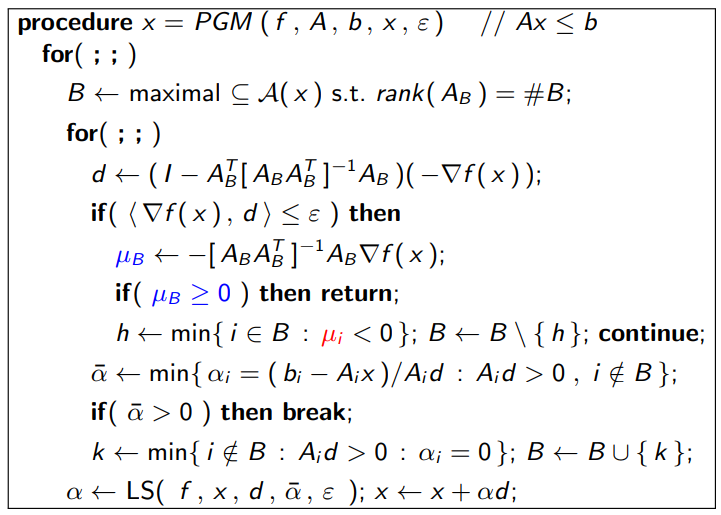
\includegraphics[scale=0.75]{12.png}
\end{center}
$\alpha_i = \max\{\alpha\:|\:A_i(x+\alpha d)\leq b_i\}$ if is $< \infty$. The pesky part is the handling of linear independence. Maximal $B$ easy to get via a greedy algorithm.
\pagebreak
\subsubsection{Frank-Wolfe Method}
Nonlinear problem with linear constraints $$(P)\:\:\min\{f(x)\:|\:Ax\leq b\}$$
Minimizing $\|x-v\|$ over $Ax\leq b$ may be too costly, but minimizing a linear function may be possible (special structure, e.g. network constraints). Solve nonlinear $(P)$ by solving a sequence of $LP$s (master problem)
\begin{center}
	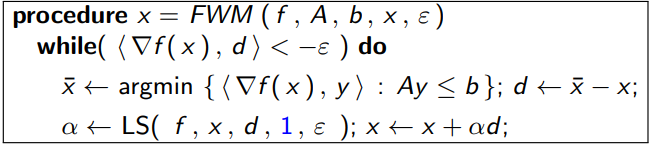
\includegraphics[scale=0.75]{13.png}
\end{center}
\begin{list}{}{}
	\item $\langle \nabla f(x),d\rangle<0 \Leftrightarrow d$ a descent direction
	\item $\langle \nabla f(x),d\rangle = 0 \Rightarrow x$ local optimum
\end{list}
$f$ convex $\Rightarrow$ $$v = f(x) + \langle \nabla f(x),d\rangle\leq v(P)$$ $\Rightarrow f(x) - v(P)\leq f(X) - v =$ readily available estimate of gap $\Rightarrow \langle \nabla f(x),d\rangle = 0 \Rightarrow x$ global optimum.
\paragraph{Stabilising the Frank-Wolfe Method} Initial $x$ not really needed: one LP, e.g. $\langle 0,y\rangle$ objective, to find it if any.\\
Convergence easy enough, similar to run-of-the-mill descent algorithm.\\
One LP per iteration is costly, exploit structure to make it efficient.\\
Convergence rather slow: trusting $L_x(\:)$ very far from $x$ where $\nabla f$ is computed.\\
Solution seen already: stabilize the master problem, but separable penalty $\gamma\|y-x\|_2$ in the objective. \textbf{Trust region stabilization}: constraint $\|y-x\|_\infty \leq \tau\Leftrightarrow$ box constraints $x_i-\tau\leq y_i\leq x_i+\tau$, almost never make an LP harder.\\
Have to manage $\tau$ somehow (e.g. fixed) but often worth it. Other ways to improve convergence speed, e.g. away step and/or use FW to identify optimal active set, then exploit it.
\paragraph{Constrained Cutting Plane (Bundle)} Stabilised Frank-Wolfe. What if $f\not\in C^1$? Cannot use $g\in\partial f(x)$, bad first order information. $f$ convex $\Rightarrow$ first-order information not so bad, globally valid.\\
What if I collect it along the way and use it all?
\begin{list}{}{}
	\item $\{x_i\}\rightarrow$ \textbf{bundle} $\mathscr{B}=\{(x_i, f_i = f(x_i), g_i\in\partial f(x_i))\} = \{(x_i, f_i, g_i)\}$
	\item \textbf{Cutting-plane model} $f_\mathscr{B}(x) = \max\{f_i+\langle g_i, x-x_i\rangle\:|\:(x_i, f_i, g_i)\in \mathscr{B}\}$, a $(1+\epsilon)$-order model.
\end{list}
$\tilde{x}\leftarrow \arg\min\{f_\mathscr{B}(x)\:|\:Ax\leq b\}$ \textbf{constrained cutting-plane algorithm}, completely equivalent to the unconstrained version, even better if $Ax\leq b$ is compact.\\
$x\leftarrow \arg\min\{f_\mathscr{B}(y)+\gamma\|y-\tilde{x}\|^2\:|\:Ay\leq b\}$ \textbf{constrained Bundle method}.\\
More difficult to exploit the structure, but not impossible.
\paragraph{Frank-Wolfe++} Sequential Quadratic Programming: want a better direction? Use a better model! Of course, second order model if you have one, or add appropriate trust region constraint to the master problem.\\
Can approximate $\nabla^2 f(x)$ with quasi-Newton formula. Fast convergence if done properly.\\
Solve a constrained quadratic program at each iteration, possibly with quadratic constraints.
\subsubsection{Dual Methods}
Quadratic program with linear constraints $$(P)\:\:\min\left\{\frac{1}{2}x^TQx+qx\:|\:Ax\leq b\right\}$$
So far, kept $Ax\leq b$ and gotten $\lambda \geq 0$ in the end. We can do the reverse (dual approach):
$$\forall\text{ fixed }\lambda\geq 0\:\:\:\psi(\lambda)=\min\left\{\frac{1}{2}x^TQx + qx + \lambda(b-Ax)\right\}\leq v(P)$$
$Q\succ 0\Rightarrow$ optimal solution $$x(\lambda)=Q^{-1}(\lambda A-q)$$
$\psi$ concave, $\psi\in C^1$, $\nabla\psi(\lambda)=b-Ax(\lambda)$\\
\textbf{Lagrangian dual}: $(D)\:\:\:\max\{\psi(\lambda)\:|\:\lambda\geq 0\}$
\begin{list}{}{}
	\item $(D)\Leftrightarrow (P)$: $v(D) = v(P)$ and $\{x(\lambda_i)\}\rightarrow x_*$ as $\{\lambda_i\}\rightarrow \lambda_*$
\end{list}
\paragraph{Dual Method} Solve $(D)$ by any method for $C^1$, but $\psi\not\in C^2$ in general. $(D)$ is constrained but the constraints are very easy (projection is trivial).\\
Feasible primal solution $x_*$ only asymptotically, but valid lower bound $v_i = \psi(\lambda_i)$ on $v(P)$ at every iteration.\\
If $X$ is "simple", then \textbf{Langragian heuristic} $X_i = p_X(x(\lambda_i))\Rightarrow$ valid upper bound $f_i = f(x_i)$ on $v(P)$ at every iteration $\Rightarrow f(x_i)-v(P)\leq f_i - v_i$ = readily available estimate of gap.\\
Can behave very differently from primal methods ($\frac{L}{\tau}$ much less of an issue). Also $Q$ singular $\Rightarrow \psi(\lambda)=-\infty$ happens $\Rightarrow$ nasty constraints in $(D)$. Extends to $f(x)$ strictly convex (must solve general nonlinear problem). $f(x)$ not convex is a serious issue, $\psi$ has to be computed exactly.
\subparagraph{Decomposition} Partial Lagrangian relaxation $$(P)\:\:\min\{f(x)\:|\:Ax\leq b, Ex\leq d\}$$
$$(R_\lambda)\:\:\:\psi(\lambda)=\min_x\{f(x)+\lambda(b-Ax)\:|\:Ex\leq d\}$$ by keeping the "easy" constraints $Ex\leq d$ and relaxing complicating constraints $Ax\leq b$
$(R_\lambda)$ is constrained but can exploit structure (and $\psi(\lambda)=-\infty$ less likely). The typical structure: $Ax\leq b$ linking constraints + $f$ separable
\begin{center}
	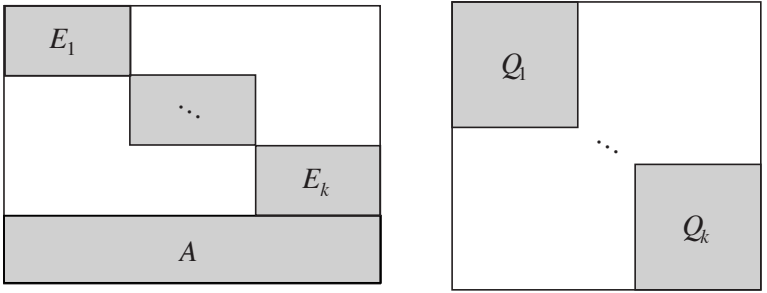
\includegraphics[scale=0.6]{14.png}\\
	$\Rightarrow \psi(\lambda)=\sum_k \psi_k(\lambda)$
\end{center}
Algorithms can exploit (parallelize).
\subsubsection{Barrier Methods}
Pro of dual method: $(D)$ is almost unconstrained (would be with $Ax = b$). The cons of dual methods are that $\psi\not\in C^2$, and even $\not\in C^1$ if $f$ isn't strictly convex, also $x(\lambda)$ is never feasible until the very end (unless Langragian heuristic).\\
We would like: unconstrained, $\in C^2$ and $x$ feasible. The first and last are obviously solved with $f + \chi_X$, but $\chi_X\not\in C^1$: we need something like $\chi_X$ but $\in C^2$. Can get $C^2$ if you accept to solve almost $(P)$ but not quite.
\paragraph{Barrier Function and Central Path} $\gamma > 0$ parameter, $(P_\gamma)\:\:\:\min\{f_\gamma(x) = f(x) - \gamma\sum_{i=1}^m \log(b_i-A_i x)\}$ \textbf{logarithmic barrier} $f_\gamma$ strictly convex (if $f$ convex), $\in C^2$ (if $f\in C^2$)
\pagebreak
\begin{multicols}{2}
\begin{center}
	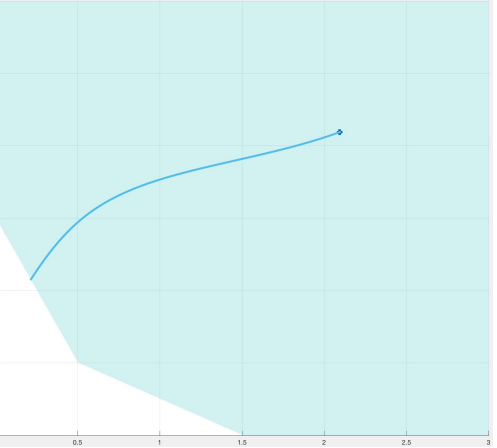
\includegraphics[scale=0.6]{15.png}
\end{center}
\begin{list}{}{}
	\item $X=\{x\in \mathbb{R}^n\:|\:Ax\leq b\}$
	\item $f_\gamma(x)=  \infty$ for $x\not\in X$ (like $\chi_X$)
	\item $f_\gamma(x)=  \infty$ for $x\in \partial X$ (unlike $\chi_X$)
	\item $\forall\:\gamma>0\:\:\exists!\:x_\gamma$ optimal of $(P_\gamma)$
	\item $x_\infty = \lim_{y\to\infty} x_\gamma$ analytic center of $X$
	\item As $\gamma \rightarrow 0$, $x_\gamma\rightarrow x_*$ analytic center of optimal face
	\item $C = \{x_\gamma\:|\:\gamma\in(0,\infty)\}$ central path (smooth curve)
\end{list}
\end{multicols}
Idea: start at center $x_\infty$ and follow $C$ to reach very close to $x_*$, always strictly feasible, never touch $\partial X$.\\\\
$f_\gamma$ is for many $f$s (linear, quadratic,\ldots). Newton's method converges very quickly to $x_\gamma$ if started within an appropriate neighborhood $N$ of $C$.\\
With $x_i$ "close" to $x(\gamma_i)$, a few Newton's steps give $x_{i+1}$ much closer to $x(\gamma_i) \Rightarrow$ "close" to $x(\gamma_{i+1})$ with $\gamma_{i+1}=\tau\gamma_i \Rightarrow$ linear convergence.\\
Overall, $O(m\log(\frac{1}{\epsilon}))$ iterations, can be made $O(\sqrt{m}\log(\frac{1}{\epsilon}))$ and more like $O(\log(m)\log(\frac{1}{\epsilon}))$ in practice. Dimension independent on $n$, not on $m$ (but almost is, in practice), but each Newton's step is at least $O(n^3)$, costly.\\
Best implementations for LP, QP, SOCP and SDP in fact are primal-dual.
\paragraph{Primal-Dual Interior-Point (Barrier) Method} Focus on quadratic case $(P)\:\:\:\min\{\frac{1}{2}x^TQx+qx\:|\:Ax\leq b\}$. Could compute Newton's step as usual.\\
Cleaner derivation out of KKT of $(P)$:
\begin{list}{}{}
	\item[(KKT-F)] $Ax + s = b$ with $s\geq 0$
	\item[(KKT-G)] $Qx + \lambda A = -q$ with $\lambda \geq 0$
	\item[(KKT-CS)] $\lambda_i s_i= 0$ for $i=1,\ldots,m$
\end{list}
One is solving the dual at the same time as the primal $(D)\:\:\:\max\{-\lambda b-\frac{1}{2}x^TQx\:|\:Qx+\lambda A= - q, \lambda \geq 0\}$\\
"Slackened KKT" characterize $x(\gamma)$ and complementarity gap:
\begin{list}{}{}
	\item With (KKT-CS-$\mu$) $\lambda_i s_i = \gamma$ for $i=1,\ldots,m \Rightarrow \sum_{i=1}^m\lambda_i s_i = \gamma m = (\frac{1}{2}x^TQx + qx)-(-\lambda b - \frac{1}{2}x^TQx)$
\end{list}
And using $\Lambda, S$ diagonal matrices with $\lambda_i, s_i$ on the diagonal, we get (KKT-CS-$\mu$) $\Lambda Su = \gamma u$ for $i=1,\ldots,m$\\\\
$x\rightarrow x + \Delta x, s\rightarrow s + \Delta s, \lambda \rightarrow \lambda + \Delta\lambda$ (current iterate plus displacement, so we get $(\Lambda + \Delta\Lambda)(S+\Delta S)u = (S\Delta\Lambda + \Lambda\Delta S + \Lambda S + \Delta\Lambda\Delta S)u = \gamma u$ so (KKT-CS-$\mu$) only nonlinear (bilinear) term $\Rightarrow$ linearize $\Leftrightarrow$ Newton's method $\Leftrightarrow$ just ignore it!
$$\left[\begin{array}{c c c}
Q&A^T&0\\
A&0&I\\
0&S&\Lambda
\end{array}\right]\left[\begin{array}{c}
\Delta x\\
\Delta \lambda\\
\Delta s
\end{array}\right]=\left[\begin{array}{c}
-(Qx+q)-\lambda A\\
b-Ax-s\\
\gamma u-\Lambda Su - \Delta\Lambda\Delta Su
\end{array}\right] \simeq \left[\begin{array}{c}
r^P\\r^D\\\gamma u-\Lambda Su
\end{array}\right] $$
\begin{center}
	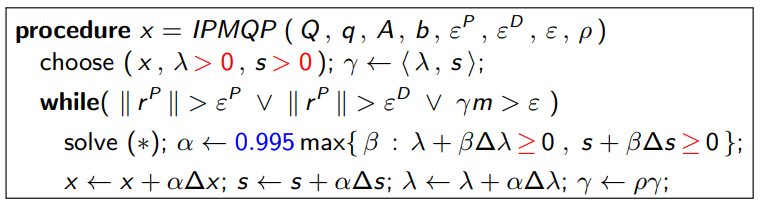
\includegraphics[scale=0.75]{17.png}
\end{center}
\begin{list}{}{}
	\item Until $\|r^P\|>\epsilon^P\vee\|r^P\|>\epsilon^D$ may choose $\alpha^P\neq \alpha^D$
	\item New iterate primal and dual feasible if the previous was, otherwise is less unfeasible than the old one
	\item Primal-dual algorithm: upper and lower bound on $v(P)$, converge as $\gamma\rightarrow 0$
	\item $\gamma = p\frac{\lambda s}{m}$ for $p<1$ fixed (a reasonable value is $p=\frac{1}{m}$)
	\item Very good convergence but large cost in time/memory per iteration
	\item May have numerical problems (dividing by very small numbers) especially on empty/unbounded problems.
\end{list}
\end{document}